\documentclass[12pt,a4paper,oneside]{report}

\usepackage[utf8]{inputenc}
\usepackage[T1]{fontenc}
\usepackage{newtxtext,newtxmath}
\usepackage{geometry}
\geometry{left=3cm,right=3cm,top=2.5cm,bottom=2.5cm}
\usepackage{setspace}
\onehalfspacing
\usepackage{microtype}
\usepackage{graphicx}
\usepackage{grffile}
\usepackage{adjustbox}
\usepackage{booktabs}
\usepackage{longtable}
\usepackage{array}
\usepackage{tabularx}
\usepackage{multirow}
\usepackage{enumitem}
\usepackage{amsmath}
\usepackage{caption}
\usepackage{subcaption}
\usepackage{xcolor}
\usepackage{hyperref}
\usepackage{cleveref}
\usepackage{fancyhdr}
\usepackage{titlesec}
\usepackage{tikz}
\usetikzlibrary{arrows.meta,positioning,shapes.geometric,fit,calc,backgrounds}
\usepackage[numbers,sort&compress]{natbib}
\usepackage{url}
\usepackage{listings}
\usepackage{float}


\definecolor{primary}{HTML}{1F4E79}
\definecolor{accent}{HTML}{2E75B6}
\definecolor{softblue}{HTML}{EAF2F8}
\definecolor{softgreen}{HTML}{EAF7EE}
\definecolor{softorange}{HTML}{FFF3E0}
\definecolor{softpurple}{HTML}{F3ECFA}
\definecolor{darkgray}{HTML}{333333}

\hypersetup{
  colorlinks=false,
  hidelinks,
  pdftitle={AI-driven Software System for Recruitment Screening using NLP and Semantic Information Retrieval},
  pdfauthor={Tran Viet Hung}
}

% Match the previous FPT thesis layout: plain pages, centered page number,
% black chapter/section headings, Times-style typeface, and generous chapter spacing.
\pagestyle{plain}
\titleformat{\chapter}[display]
  {\normalfont\bfseries\fontsize{17}{21}\selectfont}
  {\chaptertitlename\ \thechapter}{24pt}{\fontsize{17}{21}\selectfont}
\titlespacing*{\chapter}{0pt}{58pt}{48pt}
\titleformat{\section}
  {\normalfont\bfseries\fontsize{14}{17}\selectfont}
  {\thesection}{0.85em}{}
\titlespacing*{\section}{0pt}{20pt}{10pt}
\titleformat{\subsection}
  {\normalfont\bfseries\fontsize{12}{15}\selectfont}
  {\thesubsection}{0.85em}{}
\titlespacing*{\subsection}{0pt}{14pt}{7pt}
\setlength{\parindent}{0pt}
\setlength{\parskip}{0.35em}

\setlist[itemize]{topsep=3pt,itemsep=2pt,parsep=0pt}
\setlist[enumerate]{topsep=3pt,itemsep=2pt,parsep=0pt}
\captionsetup{font=small,labelfont=bf,labelsep=colon,justification=centering}
\renewcommand{\arraystretch}{1.2}

\newcommand{\systemname}{RAEMatch}
\newcommand{\thesistitle}{AI-driven Software System for Recruitment Screening using NLP and Semantic Information Retrieval}
\newcommand{\thesissubtitle}{A Ranking-based Approach for English IT CV--JD Matching}

% Thin gray border for application-screenshot figures, so their white UI
% background does not blend into the page background.
\newcommand{\appscreenshot}[1]{%
  {\setlength{\fboxsep}{0pt}\setlength{\fboxrule}{0.6pt}%
   \fcolorbox{black!35}{white}{#1}}%
}

\begin{document}

% -------------------- TITLE PAGES --------------------
\hypersetup{pageanchor=false}
\begin{titlepage}
\thispagestyle{empty}
\centering
\vspace*{0.5cm}
{\bfseries\large MINISTRY OF EDUCATION AND TRAINING\par}
\vspace{0.35cm}
{\bfseries\large FPT UNIVERSITY\par}

\vspace{3.1cm}
{\bfseries\LARGE \thesistitle\par}
\vspace{0.55cm}
{\bfseries\Large \thesissubtitle\par}

\vspace{1.35cm}
{\large by\par}
\vspace{0.45cm}
{\bfseries\large Tran Viet Hung\par}

\vspace{1.3cm}
{\large A thesis submitted in conformity with the requirements\par}
\vspace{0.35cm}
{\large for the degree of Master of Software Engineering\par}

\vfill
{\large \textcopyright\ Copyright by Tran Viet Hung 2026\par}
\end{titlepage}

\begin{titlepage}
\thispagestyle{empty}
\centering
\vspace*{0.5cm}
{\bfseries\large MINISTRY OF EDUCATION AND TRAINING\par}
\vspace{0.35cm}
{\bfseries\large FPT UNIVERSITY\par}

\vspace{2.65cm}
{\bfseries\LARGE \thesistitle\par}
\vspace{0.55cm}
{\bfseries\Large \thesissubtitle\par}

\vspace{1.15cm}
{\large by\par}
\vspace{0.4cm}
{\bfseries\large Tran Viet Hung\par}

\vspace{1.05cm}
{\large A thesis submitted in conformity with the requirements\par}
\vspace{0.3cm}
{\large for the degree of Master of Software Engineering\par}

\vspace{1.0cm}
{\large Supervisors:\par}
\vspace{0.35cm}
{\large Dr. Doan Xuan Huy Minh\par}

\vfill
{\large \textcopyright\ Copyright by Tran Viet Hung 2026\par}
\end{titlepage}

\hypersetup{pageanchor=true}
\pagenumbering{arabic}
\setcounter{page}{1}

% -------------------- ABSTRACT --------------------
\chapter*{Abstract}
\addcontentsline{toc}{chapter}{Abstract}
Recruitment screening is a high-volume information filtering problem in which recruiters must identify a small number of relevant candidates from a large collection of curriculum vitae (CVs). Existing applicant tracking systems and similarity-based methods often rely heavily on exact keywords or overall semantic similarity. Consequently, they may rank a CV highly even when the candidate does not satisfy mandatory experience, seniority, responsibility, or evidence requirements. A fresher CV, for example, may mention Java, Spring Boot, SQL, and Docker and therefore appear relevant to a senior Java role despite lacking the required years of experience, production ownership, system design, and mentoring evidence.

This thesis proposes an AI-driven recruitment screening system that formulates English IT CV--JD matching as a ranking problem and introduces a \emph{requirement-aware and evidence-aware matching mechanism with constraint-based reranking}. The system ingests PDF CVs, applies direct text extraction, and falls back to optical character recognition (OCR) for scanned documents. It then parses CV and job description (JD) content into structured sections, decomposes each JD into mandatory and optional requirements, retrieves supporting evidence from Work Experience and Projects, classifies each requirement as satisfied, partially satisfied, unsupported, or not satisfied, and validates hard constraints such as minimum years of experience and seniority level.

The experimental design combines 2,986 real scanned PDF CVs -- filtered to IT/software roles from the public Kaggle \emph{Resume Dataset PDF} \citep{hadikpresumepdf}, a general, multi-industry resume collection -- with 1,000 controlled AI-generated English IT CVs. The real corpus is used for OCR and parsing evaluation and is the majority (but not exclusive) source for the human-labeled ranking pool, while the synthetic corpus additionally supports controlled seniority-mismatch, unsupported-claim, keyword-stuffing, and scalability experiments. The primary ranking conclusions are based on a manually judged pool of 246 CV--JD pairs (138 real, 108 synthetic) across five representative Senior/Junior IT job descriptions.

The proposed approach is compared with TF--IDF, SBERT full-document similarity, and section-level SBERT baselines. Evaluation uses NDCG@5, NDCG@10, MAP, MRR, Recall@10, Recall@20, hard-constraint gating behavior, keyword-stuffing rank change, OCR reliability, and operational latency, together with bootstrap confidence intervals and a paired significance test. Against the human-labeled pool, the three similarity-only baselines rank ahead of the proposed requirement-aware, evidence-aware model on every ranking metric except MRR; this thesis reports that result directly rather than only the cases where the proposed mechanism wins, and traces it to two causes -- an auto-parsed hard-requirement list that no candidate in the top-10 ever fully satisfies (a 100\% constraint-violation rate at $k{=}10$), and evidence-similarity thresholds that a proper held-out calibration shows were left too lenient by default (calibrating them yields a genuine, held-out-validated $\sim$52\% relative improvement in NDCG@10, but closes less than a quarter of the absolute gap to the strongest baseline). A battery of controlled robustness tests, each category built as three constructed instances rather than one, shows the mechanism reliably does what it was designed to do for seniority mismatch, missing mandatory requirements, and keyword stuffing, but is fooled by descriptor-language role confusion in the majority of tested instances -- a genuine weakness the single-instance version of the same test did not reveal. The intended outcome is a practical and auditable decision-support prototype that makes requirement coverage and evidence explicit to a reviewer, improving initial CV screening while keeping final hiring decisions under human control; redesigning the JD parser's hard/optional classification and scoping declared-skill extraction to genuine personal-skill statements are identified as the two most concrete next steps rather than resolved contributions of this thesis.

\textbf{Keywords:} recruitment screening, CV--JD matching, semantic information retrieval, requirement decomposition, evidence-aware matching, constraint-based reranking, SBERT, OCR, explainable AI.

\chapter*{Acknowledgments}
\addcontentsline{toc}{chapter}{Acknowledgments}
I would like to express my sincere gratitude to my supervisor, Dr. Doan Xuan Huy Minh, for his valuable guidance, constructive feedback, and continued support throughout the development of this thesis. His comments helped me refine the research problem, improve the academic structure, and move the study beyond a simple similarity-scoring approach toward a more practical requirement-aware and evidence-aware CV--JD matching mechanism. His suggestions were especially important in clarifying the research gap, strengthening the evaluation design, and ensuring that the proposed solution remained aligned with real recruitment challenges.

I am also grateful to the lecturers of the Master of Software Engineering program at FPT University for providing the knowledge and academic foundation that supported this research. The courses in software engineering, system design, data processing, artificial intelligence, machine learning, and research methodology contributed significantly to my ability to design, implement, and evaluate the proposed system.

I would like to thank my colleagues and professional contacts who shared practical insights into recruitment screening, software development, project delivery, and technical candidate evaluation. Their perspectives helped me better understand the difficulties recruiters and technical reviewers face when assessing large numbers of CVs, especially when candidate information is incomplete, inconsistently formatted, or expressed using different technical terminology. These observations influenced the design of the requirement decomposition, evidence verification, seniority validation, and human-in-the-loop review mechanisms presented in this thesis.

I also appreciate the contributions of the reviewers and individuals who supported the evaluation preparation, including the development of representative job descriptions, relevance-labeling criteria, and feedback on candidate-ranking outputs. Their input helped make the evaluation more realistic and ensured that the proposed system was assessed not only through technical metrics but also through practical recruitment considerations.

My sincere thanks also go to the researchers, open-source communities, and dataset providers whose work made this study possible. Publicly available resume datasets, natural language processing libraries, sentence-transformer models, OCR tools, and software frameworks provided an essential foundation for implementing and evaluating the prototype in a reproducible manner.

Finally, I am deeply grateful to my family for their patience, understanding, encouragement, and emotional support throughout the research and writing process. Balancing professional responsibilities, academic work, system implementation, and experimental preparation required significant time and effort. Their continuous motivation gave me the strength to overcome difficulties and complete this thesis.

This work would not have been possible without the guidance, knowledge, support, and encouragement of all those mentioned above.

\chapter*{Statement on the Use of AI Tools}
\addcontentsline{toc}{chapter}{Statement on the Use of AI Tools}
Several figures in this thesis were generated with the assistance of AI tools (ChatGPT and Claude) rather than drawn manually or produced by a professional designer, and this is disclosed explicitly rather than left unstated. Specifically:
\begin{itemize}
  \item the conceptual architecture and process diagrams (\cref{fig:problem,fig:architecture,fig:pdfocr,fig:structuredparsing,fig:assessmentreranking,fig:reviewworkflow,fig:evaluationworkflow}) were generated from the researcher's own design descriptions and iteratively corrected for technical accuracy against the actual implementation -- for example, an earlier version of \cref{fig:pdfocr} depicted a text-cleaning step mislabeled in a way that implied personal-data anonymization the implemented system does not perform, and was regenerated to describe the step correctly;
  \item the quantitative result charts (Figures~\ref{fig:ranking-effectiveness-chart}, \ref{fig:robustness-chart}, \ref{fig:ocr-chart}, \ref{fig:performance-chart}, \ref{fig:dataset-chart}, \ref{fig:case-study-chart}) were produced by Python plotting scripts written with AI assistance, but every value plotted was computed directly from this thesis's own recorded experimental results, not generated or estimated by the AI tool;
  \item the seven application screenshots in Chapters 3--4 (\cref{fig:app-overview,fig:app-upload,fig:app-jd-parse,fig:app-ranking,fig:app-explanation,fig:app-labeling,fig:app-experiments}) were originally AI-generated mockups marked \textsc{Placeholder -- Replace with Screenshot} and have since been replaced with real screenshots of the running prototype.
\end{itemize}
All analytical content, experimental design, quantitative results, and written discussion are the researcher's own work; AI assistance was confined to the visual generation and correction of the figures listed above.

\tableofcontents
\listoffigures
\listoftables
\clearpage

% ==================================================
\chapter{Introduction}
% ==================================================

\section{Background}
Recruitment screening is one of the earliest and most time-consuming stages in the hiring process. For a single opening, recruiters may receive tens or hundreds of CVs. The challenge is particularly significant in information technology recruitment because technical roles are described using diverse terminology, abbreviations, frameworks, cloud platforms, and project responsibilities. A backend position may require Java, Spring Boot, REST APIs, microservices, SQL, Docker, Kubernetes, and cloud deployment, while candidates may describe similar experience using different phrases such as enterprise services, distributed systems, containerized deployment, or cloud-native development.

Traditional applicant tracking systems generally support keyword search, Boolean rules, and manual filters. These tools are efficient for exact matching but are sensitive to vocabulary mismatch and keyword stuffing. Semantic retrieval models reduce vocabulary mismatch by representing CVs and JDs as dense vectors. However, semantic similarity alone does not guarantee actual suitability. Two documents can be semantically related even when the candidate fails a critical requirement. A junior candidate may use the same technology stack as a senior candidate, but the depth, duration, ownership, and context of experience are different.

Therefore, the central problem is not only to calculate text similarity, but to determine whether the candidate satisfies the individual requirements of the JD and whether the CV contains supporting evidence for those requirements.

\section{Problem Statement}
Given a JD $q$ and a CV collection $D=\{d_1,d_2,\ldots,d_n\}$, a conventional ranking system calculates a relevance score $s(q,d_i)$ and returns an ordered list. This formulation is useful, but a single similarity score can hide important mismatches. For example:

\begin{itemize}
  \item a candidate may match the required skills but not the minimum years of experience;
  \item a CV may list a technology in the Skills section without evidence in Work Experience or Projects;
  \item an intern or fresher may be ranked highly for a senior role because of lexical or semantic overlap;
  \item scanned PDF extraction errors may remove important evidence and produce incorrect rankings.
\end{itemize}

The problem addressed in this thesis is therefore:

\begin{quote}
How can an AI-driven recruitment screening system rank English IT CVs for a JD by considering not only semantic similarity, but also requirement satisfaction, mandatory constraints, seniority alignment, and supporting evidence?
\end{quote}


\begin{figure}[htbp]
\centering
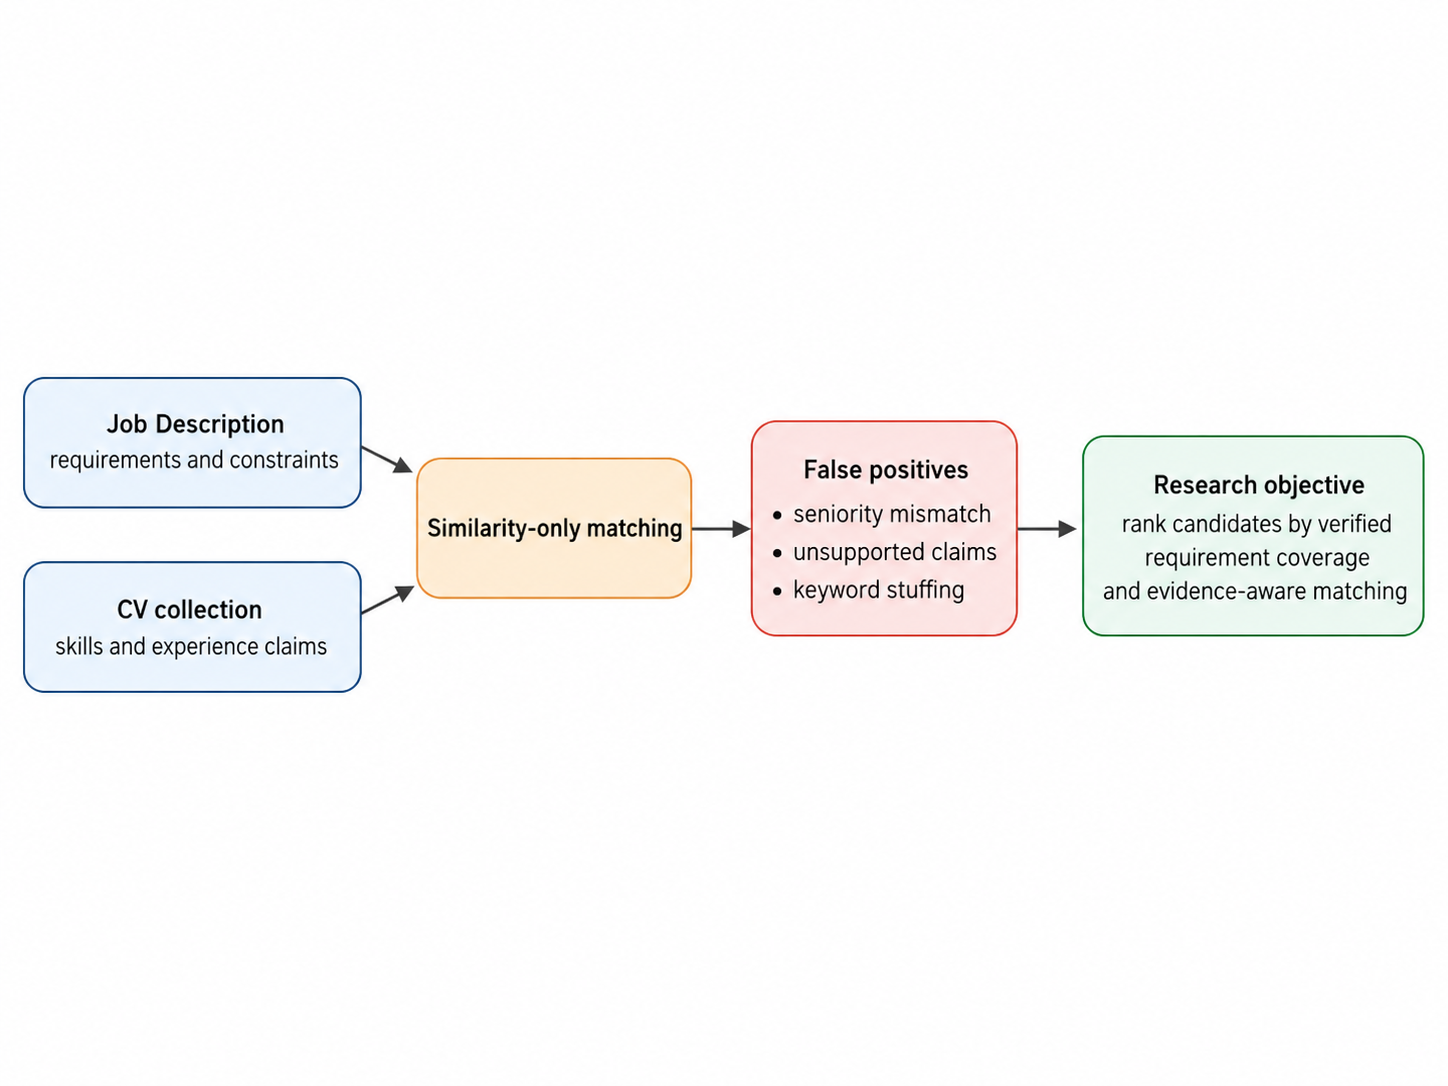
\includegraphics[width=0.98\textwidth]{figures/figure_1_1_recruitment_matching_problem_and_research_objective.png}
\caption{Recruitment matching problem and research objective}
\label{fig:problem}
\end{figure}

\section{Research Aim and Objectives}
The aim is to design and evaluate a practical recruitment screening system that performs requirement-aware and evidence-aware CV--JD matching.

The objectives are:
\begin{enumerate}
  \item Formulate English IT CV--JD matching as a ranking and information retrieval problem.
  \item Build a PDF-first CV ingestion pipeline with OCR fallback for scanned PDFs.
  \item Parse CVs and JDs into structured sections and requirements.
  \item Decompose JDs into mandatory and optional requirements.
  \item Retrieve evidence from CV Work Experience and Projects for each requirement.
  \item Validate hard constraints, including minimum experience and seniority level.
  \item Rerank candidates using verified requirement coverage rather than overall similarity alone.
  \item Evaluate the proposed mechanism using ranking metrics, robustness tests, and error analysis.
  \item Provide recruiter-facing explanations while preserving human control over hiring decisions.
\end{enumerate}

\section{Research Questions}
\begin{description}[style=nextline,leftmargin=0cm,labelsep=0pt]
  \item[RQ1] How effective are TF--IDF, SBERT full-document similarity, and section-level SBERT as baseline methods for English IT CV--JD ranking?
  \item[RQ2] Does requirement-aware matching improve ranking quality compared with similarity-only ranking?
  \item[RQ3] Does evidence-aware verification reduce false positives caused by unsupported skill claims and keyword stuffing?
  \item[RQ4] Does constraint-based reranking reduce false positives caused by experience and seniority mismatch?
  \item[RQ5] How useful and understandable are the requirement-level explanations to recruiters or technical reviewers during candidate review?
\end{description}

\section{Scope and Exclusions}
The scope is intentionally limited to English IT recruitment and initial CV screening. The system prioritizes review order and provides evidence; it does not make final hiring or rejection decisions.

\begin{table}[htbp]
\centering
\caption{Research scope and exclusions}
\label{tab:scope}
\begin{tabularx}{\textwidth}{>{\bfseries}p{0.20\textwidth}XX}
\toprule
Dimension & Included & Excluded or Future Work \\
\midrule
Language & English CVs and JDs & Vietnamese and multilingual matching \\
Domain & IT roles such as developer, QA, DevOps, data, BA, PM, and architect & Non-IT recruitment \\
Input & PDF CVs with direct extraction and OCR fallback & Unsupported office and image formats as primary inputs \\
Dataset & Real scanned Kaggle PDFs and controlled AI-generated English IT CVs & Private company CV databases \\
Task & Top-$k$ ranking and recruiter decision support & Automatic hiring or rejection \\
Matching & Requirement-aware, evidence-aware, constraint-based reranking & External employment or credential verification \\
Ground truth & Human relevance judgments and controlled robustness metadata & Fully automatic relevance labeling \\
Models & TF--IDF, SBERT, section-level SBERT, and the proposed mechanism & Large-scale model fine-tuning and production ATS integration \\
Evaluation & Ranking metrics, ablation, robustness, OCR, latency, and explanation usability & Long-term employee performance prediction \\
\bottomrule
\end{tabularx}
\end{table}

\section{Main Contributions}
The thesis contributes:
\begin{enumerate}
  \item a modular software architecture for PDF ingestion, OCR fallback, structured parsing, requirement decomposition, evidence retrieval, constraint validation, reranking, and explanation;
  \item a requirement-level representation that classifies each JD requirement as satisfied, partially satisfied, unsupported, or not satisfied;
  \item an explicit distinction between declared skills and evidence-supported skills in Work Experience and Projects;
  \item explicit treatment of minimum experience and seniority as constraints rather than generic semantic similarity;
  \item a deterministic lexicographic reranking mechanism that prevents broad similarity from compensating for failed mandatory requirements;
  \item a mixed real-and-synthetic experimental design that separates real-world OCR and human-labeled ranking evaluation from controlled robustness and scalability testing;
  \item recruiter-oriented explanations that present requirement coverage, evidence sentences, gaps, and warnings;
  \item an evaluation protocol covering effectiveness, ablation, seniority mismatch, keyword stuffing, OCR quality, operational latency, and explanation usability.
\end{enumerate}

The novelty is not a new foundation language model. It is the design and validation of an auditable matching mechanism that changes the unit of comparison from whole-document similarity to individual JD requirements and their supporting CV evidence. This distinction links the algorithmic behavior, software architecture, recruiter workflow, and evaluation criteria to the original recruitment problem.

\section{Thesis Structure}
The remainder of the thesis is organized into four chapters. Chapter 2 reviews relevant literature. Chapter 3 presents the system design and implementation. Chapter 4 describes the evaluation and discusses the results. Chapter 5 concludes the thesis and proposes future work.

% ==================================================
\chapter{Literature Review}
% ==================================================

\section{Recruitment Screening and Applicant Tracking Systems}
Applicant tracking systems support CV storage, filtering, keyword search, and workflow management. Keyword and Boolean filters are efficient and interpretable, but they are vulnerable to vocabulary mismatch and keyword stuffing. A candidate may be relevant without using the exact terms in the JD, while another candidate may list many keywords without demonstrating practical experience. Comparative studies of semantic resume-to-job matching report similar vocabulary-mismatch and evidence-verification gaps in existing CV--JD systems \citep{alderham2022}.

\section{Information Retrieval for CV--JD Matching}
In information retrieval, the JD is treated as a query and the CV collection as documents. TF--IDF remains a useful lexical baseline because exact technical terms often matter in IT recruitment \citep{salton1988}. Cosine similarity between TF--IDF vectors is efficient and transparent. BM25 improves lexical retrieval through term saturation and document-length normalization, but it is not the main implementation in this thesis and remains a future extension \citep{manning2008,robertson2009}.

\section{Semantic Retrieval and SBERT}
Transformer-based embeddings capture semantic relationships beyond exact words, building on the self-attention architecture introduced for sequence modeling \citep{vaswani2017}. BERT introduced contextual bidirectional representations \citep{devlin2019}, while Sentence-BERT enables efficient sentence and document similarity by producing comparable embeddings \citep{reimers2019}. SBERT is suitable for first-stage retrieval because CV and JD embeddings can be precomputed and compared efficiently.

However, full-document similarity has limitations. Long CVs may contain unrelated content, and a high semantic score can be produced by broad topical overlap. Section-level matching reduces this problem by comparing relevant sections, such as Skills and Work Experience, separately.

\section{Cross-Encoder and Reranking Approaches}
Two-stage retrieval architectures commonly use a fast bi-encoder to retrieve a candidate set and a more expensive reranker to refine ordering. Cross-encoders jointly process query-document pairs and often provide stronger interaction modeling than independent embeddings. Learning-to-rank methods such as LambdaMART can combine multiple relevance signals, but they require sufficient labeled data. Given the time and data limitations of this thesis, the proposed system uses deterministic requirement-level reranking and places trainable learning-to-rank in future work.

\section{Requirement Decomposition and Constraint Matching}
A JD is not a single homogeneous text. It contains mandatory skills, optional skills, minimum experience, seniority, responsibilities, education requirements, and certifications. Treating these requirements independently is closer to recruiter practice. Hard constraints determine whether a candidate satisfies critical conditions, while soft constraints affect preference without necessarily excluding the candidate.

Constraint-aware matching is especially important for seniority. Semantic similarity between a senior JD and a junior CV may be high if both mention the same technologies. A dedicated seniority check can identify this mismatch directly.

\section{Evidence-aware Matching and Unsupported Claims}
A CV may declare skills without providing evidence. It is not possible to determine whether a CV is fraudulent using the document alone, but it is possible to identify \emph{unsupported claims}. Evidence-aware matching searches Work Experience and Project sections for sentences that support a declared skill or responsibility. This distinction reduces ranking inflation caused by keyword stuffing.

The evidence problem can be represented as:
\begin{equation}
E(r,d)=\max_{s\in \mathcal{S}(d)} \operatorname{sim}(r,s),
\end{equation}
where $r$ is a JD requirement, $\mathcal{S}(d)$ is the set of evidence sentences extracted from CV $d$, and $\operatorname{sim}$ is a semantic similarity function. If no sentence exceeds a threshold, the requirement is marked unsupported or not satisfied.

\section{Resume Parsing, PDF Extraction, and OCR}
CV documents often contain multiple columns, icons, tables, and irregular headings. Text-based PDFs can be parsed using libraries such as PyPDF or pdfplumber. Scanned PDFs require OCR, for which Tesseract provides an established open-source engine architecture \citep{smith2007tesseract}. OCR may introduce character errors, broken lines, and section boundary problems, which can affect ranking quality. Therefore, the ingestion pipeline should record extraction status, text length, and parsing warnings.

\section{Explainability and Human Control}
Recruitment systems require transparency because screening affects individuals. Practical explanations should show job-relevant evidence that recruiters can verify. Model-agnostic explanation techniques such as LIME show that post-hoc, locally faithful explanations can be produced without exposing internal model weights \citep{ribeiro2016}, but attention heatmaps alone are not sufficient because attention is not necessarily a faithful explanation of model behavior \citep{jacovi2020}. The proposed system therefore explains ranking through requirement status, missing constraints, seniority gaps, and supporting sentences.

\section{Comparison of Related Approaches}
Table~\ref{tab:related-work} summarizes the main methodological families relevant to this thesis. Lexical and dense retrieval methods are effective for candidate discovery but do not directly verify requirement satisfaction. Cross-encoders and learning-to-rank methods improve interaction modeling, but they normally require additional computation or labeled training data. The proposed mechanism focuses on requirement decomposition, evidence verification, and explicit constraint handling while remaining deterministic and auditable.

\begin{table}[htbp]
\centering
\caption{Comparison of related CV--JD matching approaches}
\label{tab:related-work}
\begin{tabularx}{\textwidth}{p{0.18\textwidth}p{0.18\textwidth}p{0.16\textwidth}XX}
\toprule
Approach & Main signal & Typical output & Strength & Limitation relative to this work \\
\midrule
Keyword / TF--IDF & Exact term overlap & Similarity rank & Fast and interpretable & Vocabulary mismatch; vulnerable to keyword stuffing \\
Dense bi-encoder / SBERT & Global semantic similarity & Similarity rank & Handles paraphrases and related wording & Can hide mandatory, seniority, and evidence gaps \\
Section-level matching & Section-specific semantic similarity & Weighted rank & Reduces dilution from unrelated CV content & Usually remains score-centric and does not verify each requirement \\
Cross-encoder reranking & Joint CV--JD interaction & Relevance score & Strong pairwise interaction modeling & Higher latency; difficult to audit without evidence extraction \\
Learning-to-rank & Learned feature combination & Learned rank & Learns feature importance from labels & Requires sufficient representative labeled query groups \\
Proposed mechanism & Requirement states, evidence, constraints & Auditable rank & Prioritizes mandatory fit and supported evidence & Rule and threshold quality must be calibrated and evaluated \\
\bottomrule
\end{tabularx}
\end{table}

\section{Synthetic Data for Controlled Evaluation}
Synthetic data can supplement limited real-world corpora by creating controlled combinations of role, seniority, experience, skill evidence, and adversarial cases. However, AI-generated text may contain stylistic artifacts, overly clean language, or patterns inherited from the generation prompt. Therefore, synthetic CVs should support robustness and scalability analysis rather than replace human judgment on real CVs. Recent work on LLM-driven synthetic data emphasizes the need for transparent generation protocols, quality controls, source separation, and careful interpretation of downstream results \citep{long2024synthetic,tan2024annotation}.

In this thesis, synthetic CVs are generated from structured candidate profiles rather than copied from target JDs. Each record retains provenance and scenario metadata, allowing controlled tests for seniority mismatch, missing mandatory skills, unsupported claims, and keyword stuffing. Primary claims about real-world matching remain grounded in manually judged CV--JD pairs.

\section{Research Gap}
The literature provides strong methods for lexical retrieval, semantic retrieval, and ranking. However, many CV--JD systems still optimize a global similarity score. They may not explicitly distinguish mandatory from optional requirements, validate seniority constraints, or verify whether claimed skills are supported by experience evidence.

The gap addressed by this thesis is a practical multi-stage mechanism that:
\begin{itemize}
  \item decomposes the JD into explicit requirements;
  \item retrieves evidence for each requirement from CV sections;
  \item distinguishes declared skills from evidenced skills;
  \item validates minimum experience and seniority constraints;
  \item reranks candidates based on requirement coverage and constraint satisfaction;
  \item explains each decision to the recruiter.
\end{itemize}

% ==================================================
\chapter{System Design and Implementation}
% ==================================================

\section{System Overview}
The proposed system, named \systemname{}, is a recruiter-facing decision-support prototype. Its main workflow is shown in \cref{fig:architecture}. The system separates document ingestion, structured parsing, matching, reranking, and explanation into independent modules.

\begin{figure}[htbp]
\centering
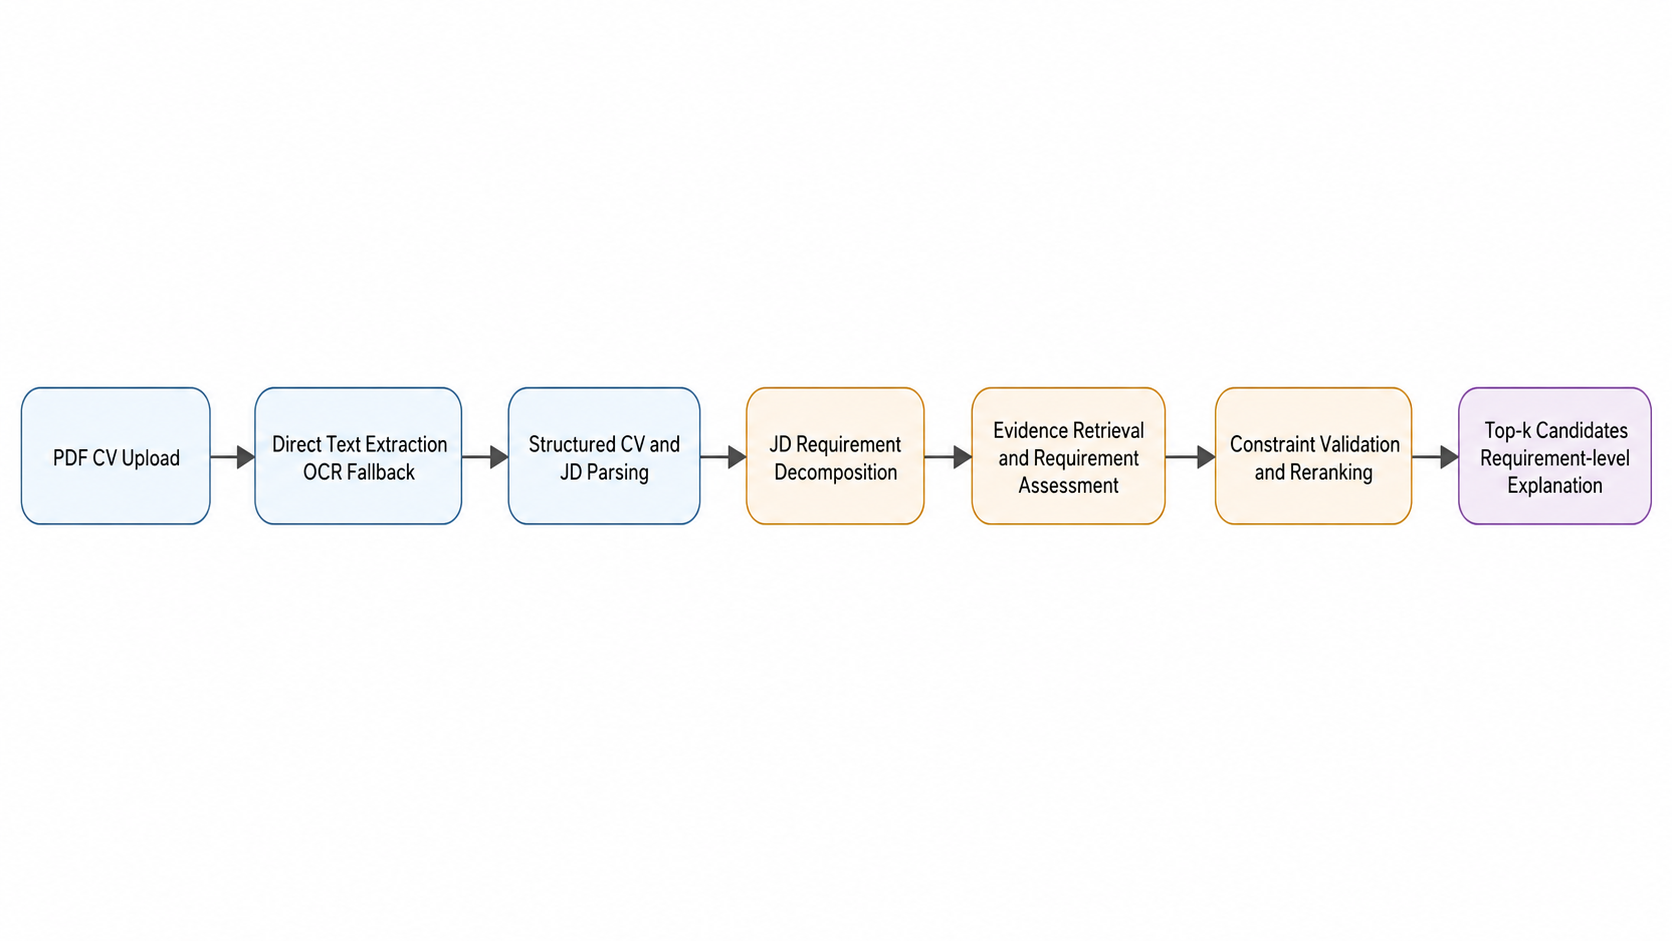
\includegraphics[width=0.98\textwidth]{figures/figure_3_1_requirement_aware_evidence_aware_matching_architecture.png}
\caption{Proposed requirement-aware and evidence-aware matching architecture}
\label{fig:architecture}
\end{figure}

\Cref{fig:app-overview} shows the running prototype's Ranking-tab landing view, the concrete counterpart to the architecture diagram above: the \emph{Import CVs} card (source-type selector, PDF drop zone, and the live indexed-CV count) and the \emph{Create JD} card (Upload PDF vs.\ Manual form) side by side, the two entry points into every subsequent pipeline stage described in this chapter.

\begin{figure}[htbp]
\centering
\appscreenshot{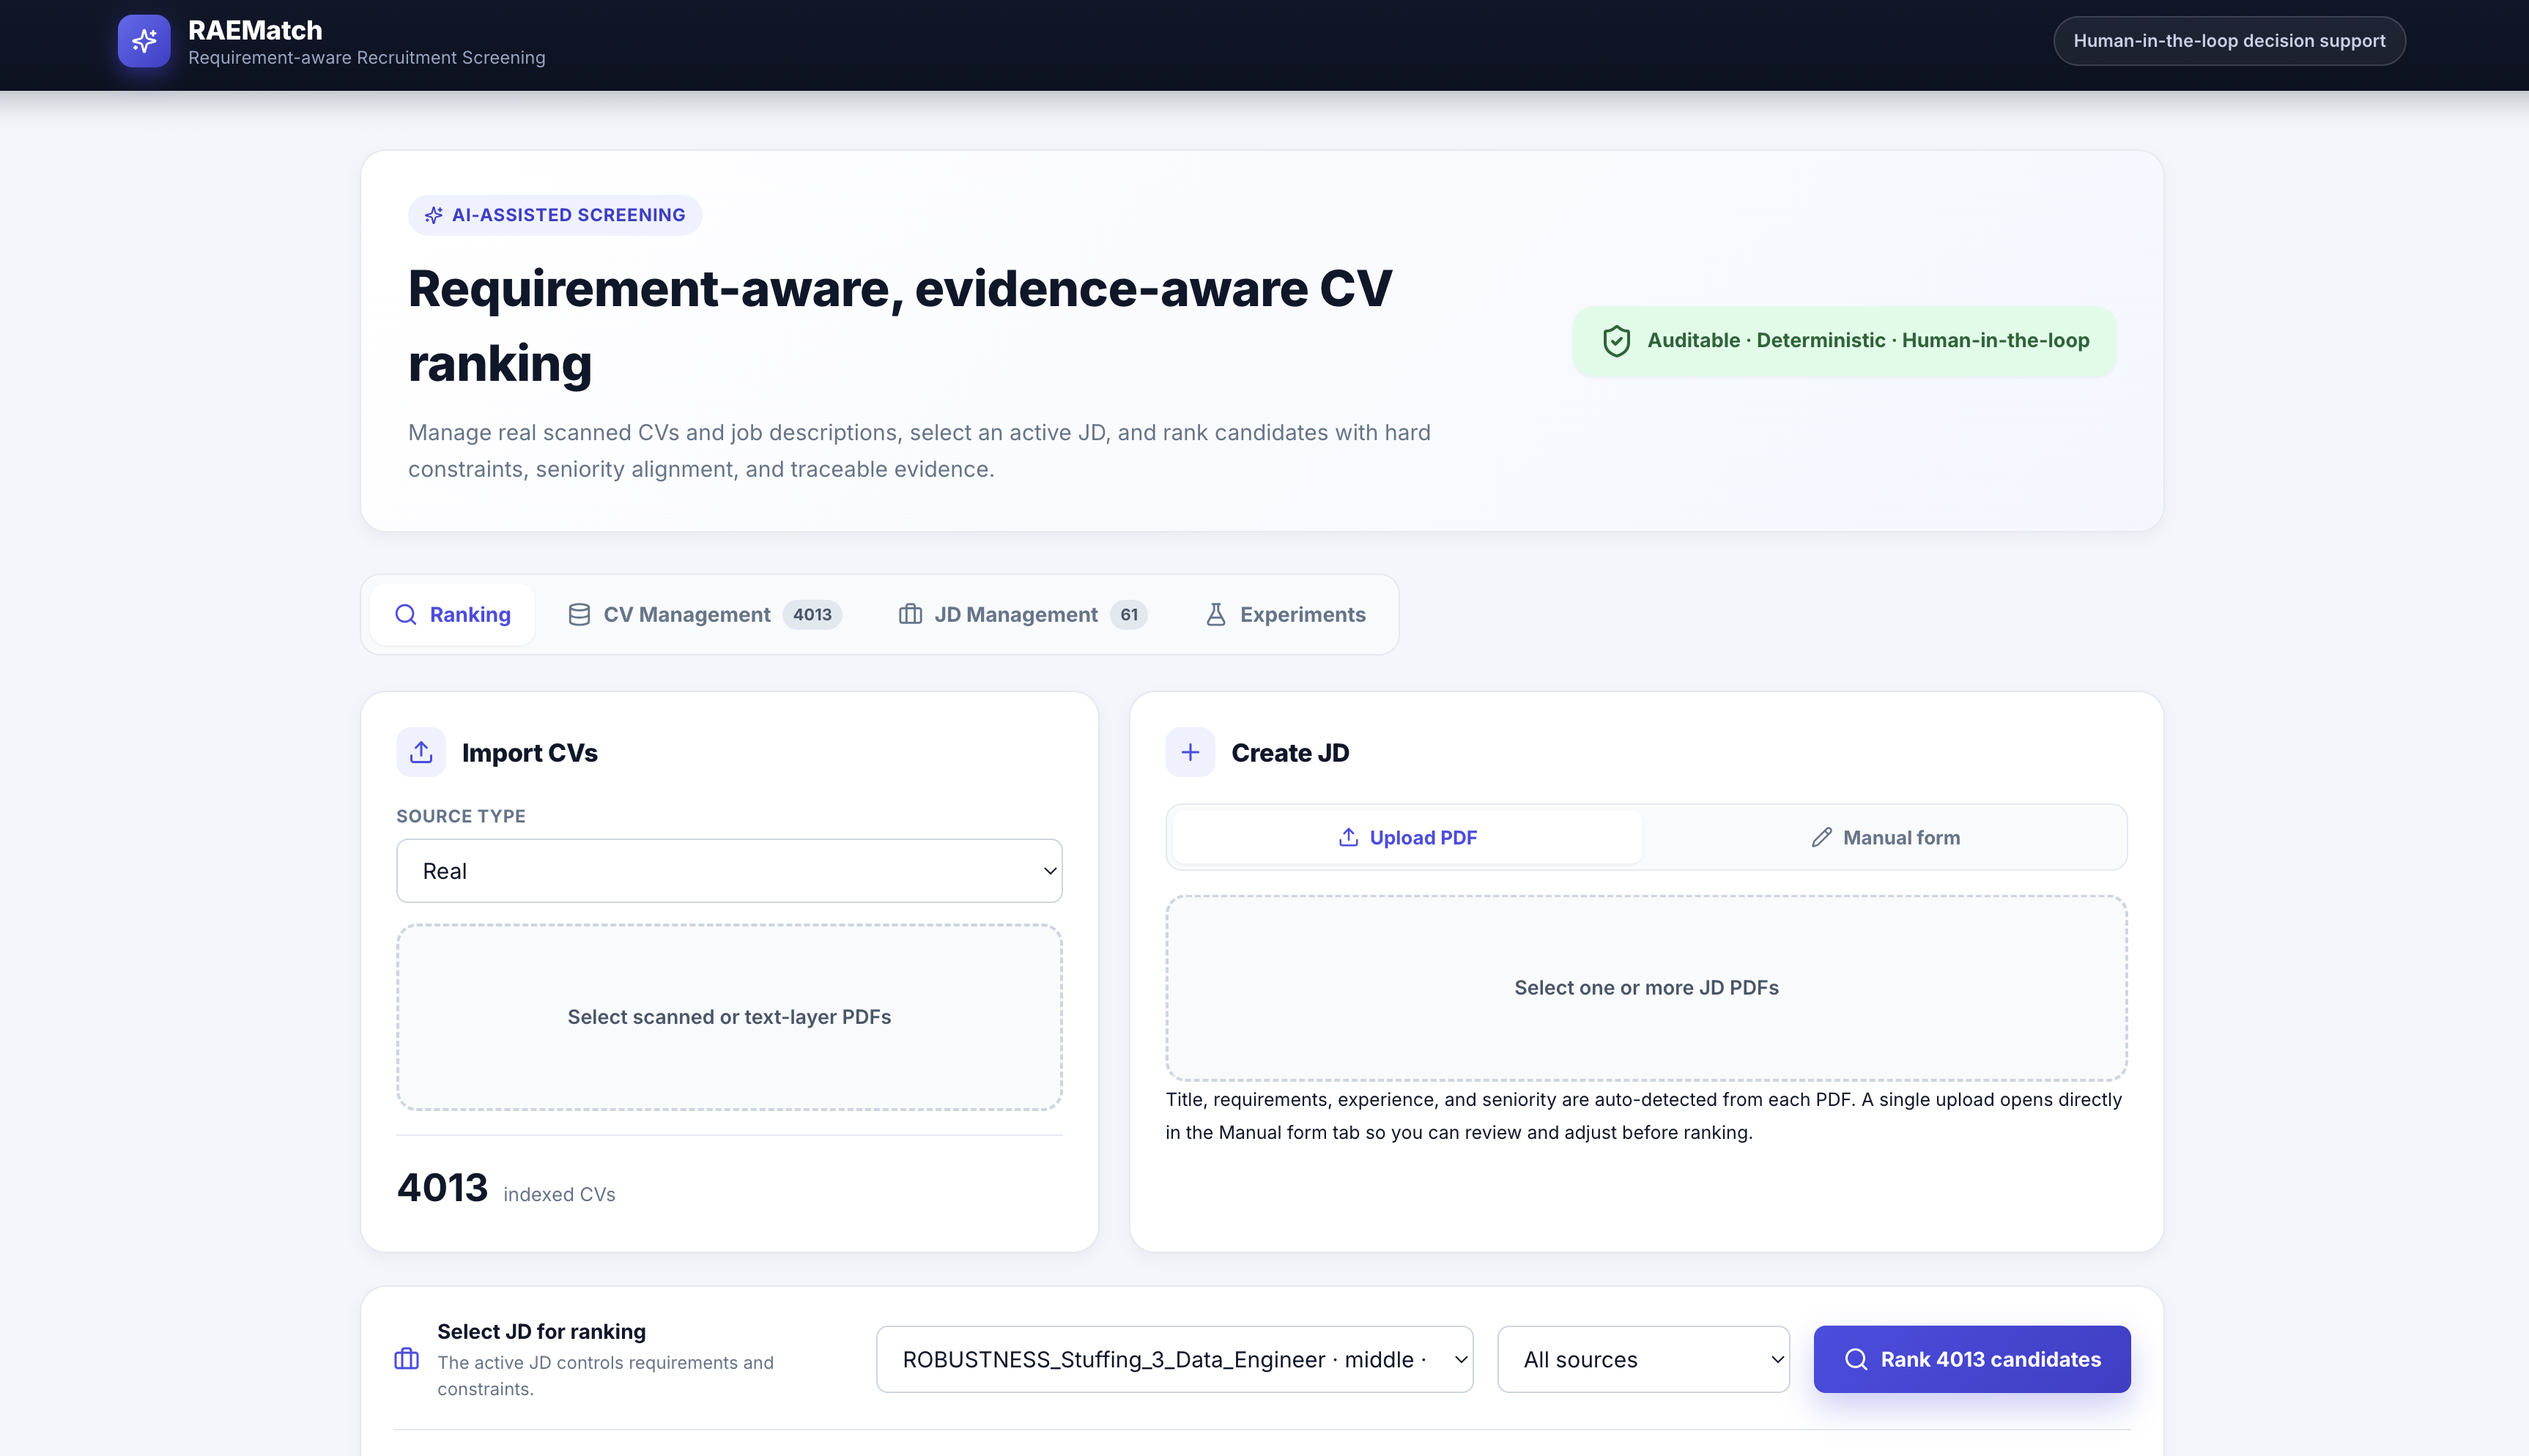
\includegraphics[width=0.98\textwidth]{figures/figure_3_2_app_overview_import_cvs_and_create_jd.png}}
\caption{Application overview: Import CVs and Create JD}
\label{fig:app-overview}
\end{figure}

\section{Functional Requirements}
The system shall:
\begin{enumerate}
  \item upload one or more PDF CV files;
  \item extract text directly or apply OCR fallback;
  \item parse CV sections and JD requirements;
  \item classify requirements as mandatory or optional;
  \item extract experience years and seniority levels;
  \item retrieve supporting evidence sentences;
  \item assess requirement satisfaction;
  \item rerank candidates using hard and soft constraints;
  \item show top-$k$ results and explanations;
  \item store reviewer relevance labels and evaluation results.
\end{enumerate}

\subsection{Non-functional Requirements}
The prototype targets five non-functional requirements: traceability, deterministic behavior, privacy protection, acceptable response time, and modularity. Every ranking result retains the parsed requirements, requirement states, evidence sentences, constraint violations, and baseline tie-breaker, so a reviewer can reproduce why a candidate landed at a given rank. Parsing, evidence retrieval, constraint validation, reranking, and explanation generation are separate, independently testable modules. Privacy protection is currently a design goal rather than a delivered control: direct identifiers are not masked before ranking, and the built-in CV viewer displays the original, unredacted PDF (\cref{sec:security}; Chapter 5, Limitations).

\section{PDF Ingestion and OCR Fallback}
\label{sec:pdf-ingestion}
The main user-facing input is PDF. Direct extraction is attempted first because it is faster and generally more accurate for text-based PDFs. If the extracted text is empty or below a minimum quality threshold, the system renders the PDF pages and applies OCR.

\begin{figure}[htbp]
\centering
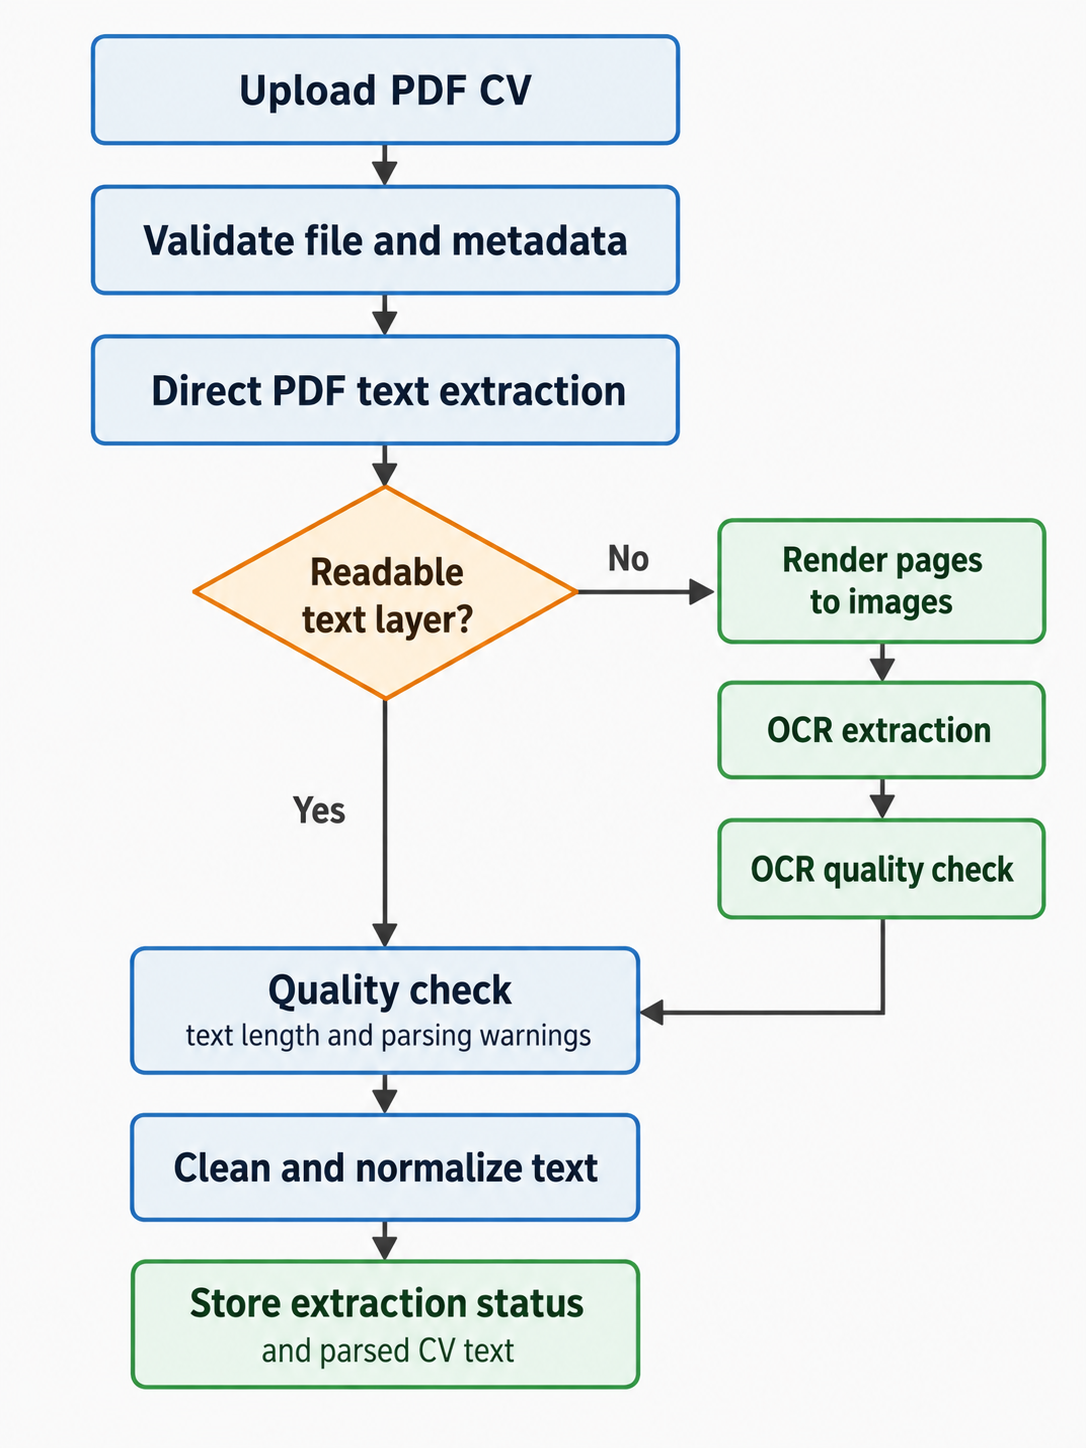
\includegraphics[width=0.68\textwidth,keepaspectratio]{figures/figure_3_3_pdf_ingestion_and_ocr_fallback_process.png}
\caption{PDF ingestion and OCR fallback process}
\label{fig:pdfocr}
\end{figure}

Each upload returns a per-file status: \texttt{pdf\_\allowbreak text\_\allowbreak extracted} or \texttt{pdf\_\allowbreak ocr\_\allowbreak extracted} on success, or one of \texttt{pdf\_\allowbreak only} (non-PDF file), \texttt{empty\_\allowbreak file}, \texttt{ocr\_\allowbreak empty}, or \texttt{ocr\_\allowbreak unavailable\_\allowbreak or\_\allowbreak failed} on failure. Unreadable files are excluded from ranking rather than silently assigned low relevance; the current build does not, however, persist a count of rejected files (see Limitations, Chapter 5).

\Cref{fig:app-upload} shows the Ranking tab's \emph{Import CVs} card after uploading a batch of real scanned PDFs, together with the CV Management table's \emph{Extraction} column for those records, making the direct-extraction/OCR-fallback distinction above visible for a mixed batch.

\begin{figure}[htbp]
\centering
\appscreenshot{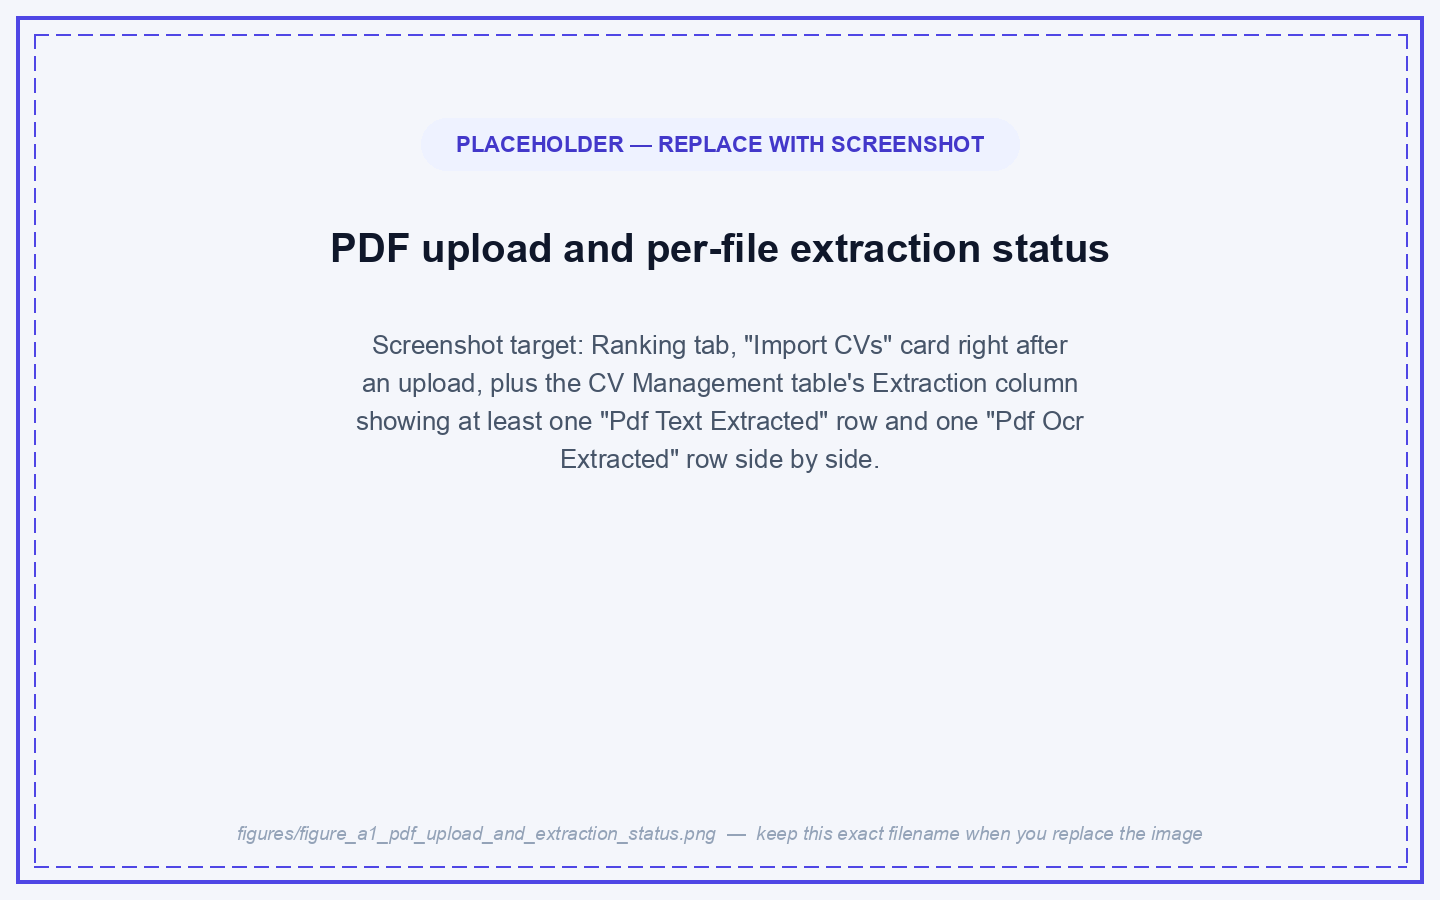
\includegraphics[width=0.92\textwidth]{figures/figure_3_4_pdf_upload_and_extraction_status.png}}
\caption{PDF upload and per-file extraction status}
\label{fig:app-upload}
\end{figure}

\section{Structured CV and JD Parsing}
\label{sec:cv-jd-parsing}
The parser normalizes CV headings and extracts the following sections:
\begin{itemize}
  \item Summary or Career Objective;
  \item Skills;
  \item Work Experience;
  \item Projects;
  \item Education;
  \item Certifications.
\end{itemize}

The JD parser extracts job title, mandatory skills, optional skills, minimum years, required seniority, responsibilities, education, and certifications. A rule-based parser is used for the prototype because it is deterministic and auditable. Skill dictionaries and heading synonyms are configurable.


\begin{figure}[htbp]
\centering
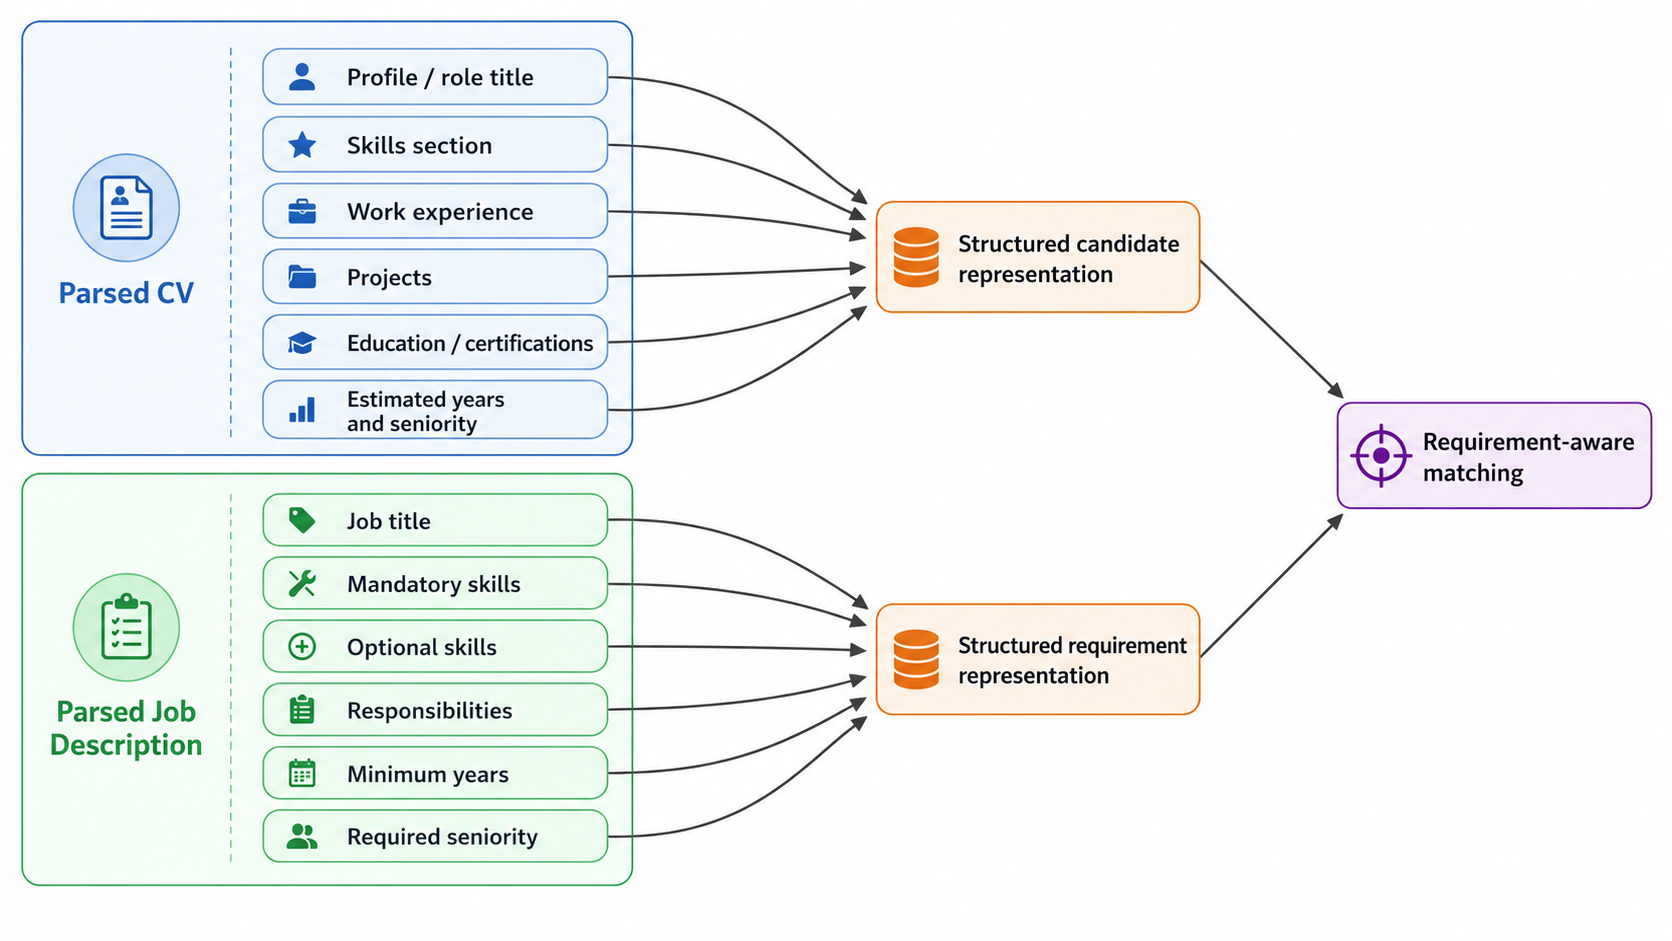
\includegraphics[width=0.98\textwidth]{figures/figure_3_5_structured_parsing_output_for_cv_and_jd_documents.png}
\caption{Structured parsing output for CV and JD documents}
\label{fig:structuredparsing}
\end{figure}

\Cref{fig:app-jd-parse} shows the resulting JD Management card for a JD created via the \emph{Upload PDF} path from a job posting with clear Requirements/Nice-to-have/Responsibilities/Education headings: the card lists both hard (red) and soft (blue) requirement chips with non-zero counts of each, evidence that the rule-based parser distinguishes mandatory from optional requirements rather than flattening everything to a single skill list.

\begin{figure}[htbp]
\centering
\appscreenshot{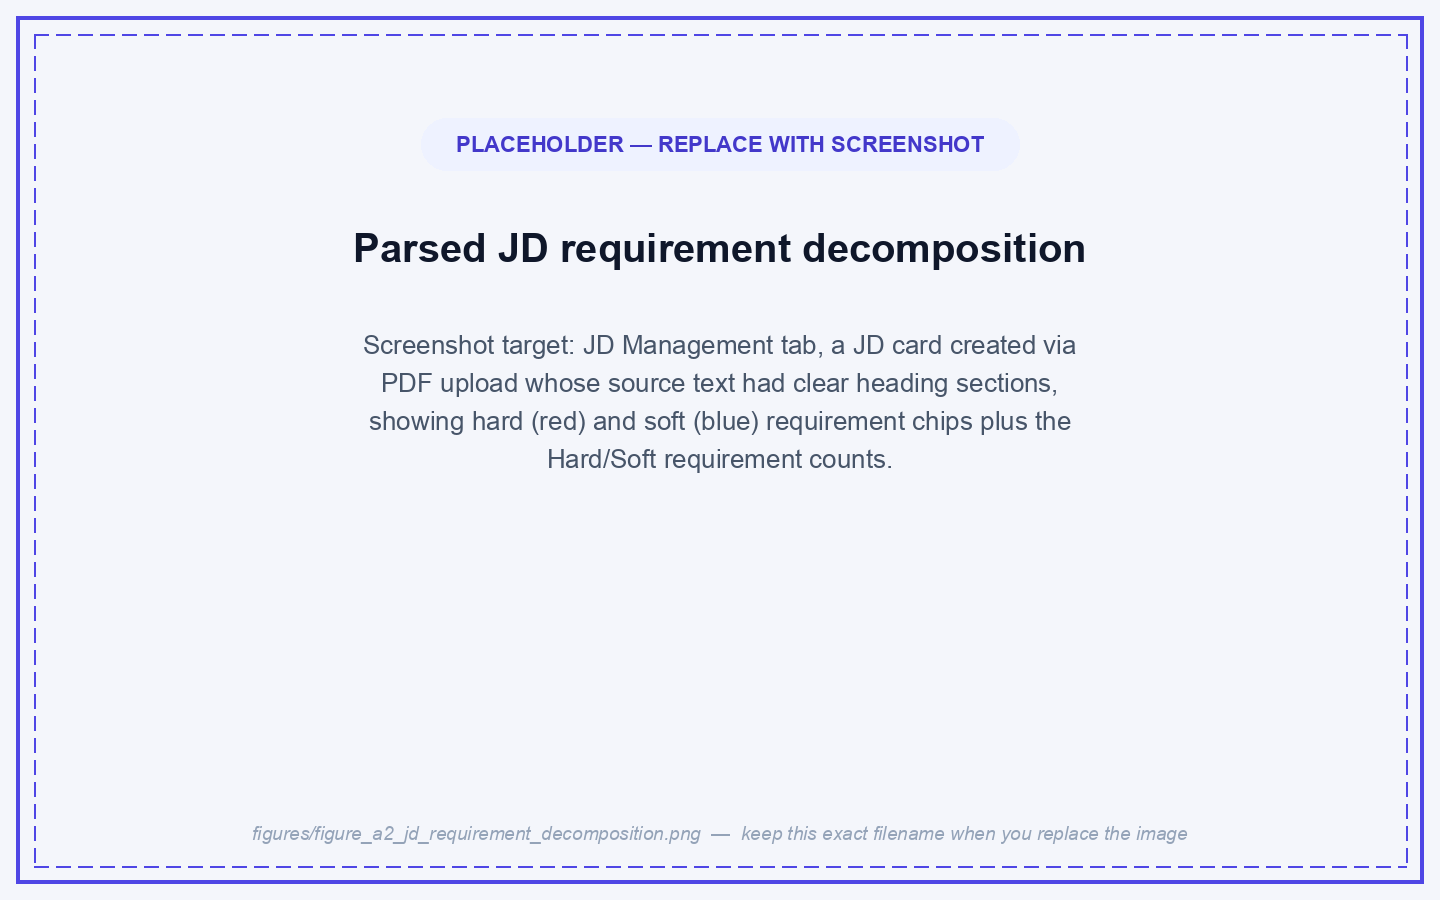
\includegraphics[width=0.92\textwidth]{figures/figure_3_6_jd_requirement_decomposition.png}}
\caption{Parsed JD requirement decomposition}
\label{fig:app-jd-parse}
\end{figure}

\begin{table}[htbp]
\centering
\caption{Structured representation of a job description}
\label{tab:jdstructure}
\begin{tabularx}{\textwidth}{>{\bfseries}p{0.28\textwidth}X}
\toprule
Field & Example \\
\midrule
Job title & Senior Java Developer \\
Mandatory skills & Java, Spring Boot, REST API, SQL \\
Optional skills & AWS, Kubernetes, Kafka \\
Minimum experience & 5 years \\
Required seniority & Senior \\
Responsibilities & System design, production troubleshooting, mentoring \\
Education/certification & Bachelor degree; cloud certification preferred \\
\bottomrule
\end{tabularx}
\end{table}

\section{Dataset Provenance and Source Tracking}
Every CV record retains a source type (\texttt{real} or \texttt{synthetic}) and an extraction status, so real and synthetic results can be analyzed separately and the ranking/experiment endpoints filtered to a single subset (Table~\ref{tab:provenance}). Scenario metadata (e.g., seniority-mismatch or keyword-stuffing labels) and a development/evaluation/robustness/scalability split are planned for the controlled robustness sets but are not yet columns in the CV record; until added, those subsets must be tracked externally (e.g., a candidate-id list) rather than queried directly.

\begin{table}[htbp]
\centering
\caption{Core provenance fields, current implementation status}
\label{tab:provenance}
\begin{tabularx}{\textwidth}{>{\bfseries}p{0.25\textwidth}p{0.18\textwidth}p{0.18\textwidth}X}
\toprule
Field & Real PDF example & Synthetic example & Status \\
\midrule
CV identifier & \texttt{REAL\_\allowbreak <hex10>} & \texttt{SYN\_\allowbreak <hex10>} & Implemented \\
Source type & \texttt{real} & \texttt{synthetic} & Implemented (\texttt{CV.\allowbreak source\_\allowbreak type}) \\
Extraction status & \texttt{pdf\_\allowbreak ocr\_\allowbreak extracted} & \texttt{pdf\_\allowbreak text\_\allowbreak extracted} & Implemented (\texttt{CV.\allowbreak parse\_\allowbreak status}); also used as a document-type proxy (OCR implies a scanned source, direct extraction implies a text-layer source) \\
Role / seniority & Parsed from CV & Parsed from CV & Implemented \\
Experience years & Parsed from CV & Parsed from CV & Implemented \\
Evidenced / unsupported skills & Computed against a given JD at ranking time & Computed against a given JD at ranking time & Implemented, but computed dynamically per JD--CV pair, not stored as a static per-CV field \\
Scenario type (e.g. seniority mismatch, keyword stuffing) & -- & -- & Not implemented -- planned for the controlled robustness sets \\
Experiment split (development/evaluation/robustness/scalability) & -- & -- & Not implemented -- planned for the controlled robustness sets \\
\bottomrule
\end{tabularx}
\end{table}

\section{Synthetic CV Generation Protocol}
Approximately 1,000 English IT CVs are generated from structured candidate profiles using ChatGPT (GPT-4/GPT-4o family) to increase corpus scale and create controlled edge cases. The exact model version, prompt template, and generation date remain \texttt{Pending external input} since they were not recorded at generation time. The protocol is fixed as follows:
\begin{enumerate}
  \item define role, seniority, years of experience, responsibilities, evidenced skills, declared-only skills, education, and certifications;
  \item generate CV text without exposing or copying the target evaluation JD;
  \item convert the generated record into a consistent PDF format and retain a machine-readable manifest;
  \item reject empty, duplicated, internally inconsistent, or excessively repetitive outputs;
  \item sample records manually for language quality and profile consistency;
  \item retain source-type provenance (\texttt{real}/\texttt{synthetic}) on every record so real and synthetic results \emph{can} be separated at analysis time.
\end{enumerate}

This last point states intent rather than a fully realized separation: despite retaining provenance, the primary 246-pair human-labeled effectiveness pool itself mixes 138 real and 108 synthetic CVs and is scored as one combined macro-average (\cref{sec:labeled-pool}, Table~\ref{tab:ranking-results}), so synthetic CVs do directly influence the headline ranking-effectiveness result rather than being confined to the separate robustness and scalability sets. This is reported as a deviation from the original design intent, not silently reconciled with it, and is listed as a limitation (\cref{sec:limitations-list}).

The role matrix includes backend, frontend, full-stack, QA automation, DevOps, data engineering, business analysis, project management, software architecture, and IT support. The seniority matrix includes Intern, Fresher, Junior, Middle, Senior, Lead, and Architect. The final role and seniority distribution across the 1,000 generated CVs was not recorded and remains \texttt{Pending external input} (\cref{sec:limitations-list}).

\section{Requirement Decomposition}
Each JD is converted into a set of atomic requirements:
\begin{equation}
R(q)=R_h(q)\cup R_s(q),
\end{equation}
where $R_h$ contains hard constraints and $R_s$ contains soft preferences.

Examples of hard constraints are mandatory skills, minimum years, and required certification. Soft constraints include optional tools, preferred education, or desirable domain experience.

Each requirement is represented as:
\begin{equation}
r_j=(t_j,c_j,w_j),
\end{equation}
where $t_j$ is the requirement text, $c_j\in\{\text{hard},\text{soft}\}$ is the constraint type, and $w_j$ is its importance.

\section{Candidate Evidence Retrieval}
The system splits Work Experience and Project sections into evidence sentences. For each requirement $r_j$, it calculates semantic similarity against all evidence sentences and retrieves the most relevant sentence:
\begin{equation}
s_j^*=\arg\max_{s\in \mathcal{S}(d)} \operatorname{cos}(\mathbf{e}_{r_j},\mathbf{e}_s).
\end{equation}

The evidence score is:
\begin{equation}
E_j=\max_{s\in \mathcal{S}(d)} \operatorname{cos}(\mathbf{e}_{r_j},\mathbf{e}_s).
\end{equation}

A skill listed only in the Skills section is considered \emph{declared}. It becomes \emph{evidenced} only when a supporting sentence is found in Work Experience or Projects above the selected threshold.

\section{Requirement Satisfaction Assessment}

\begin{figure}[htbp]
\centering
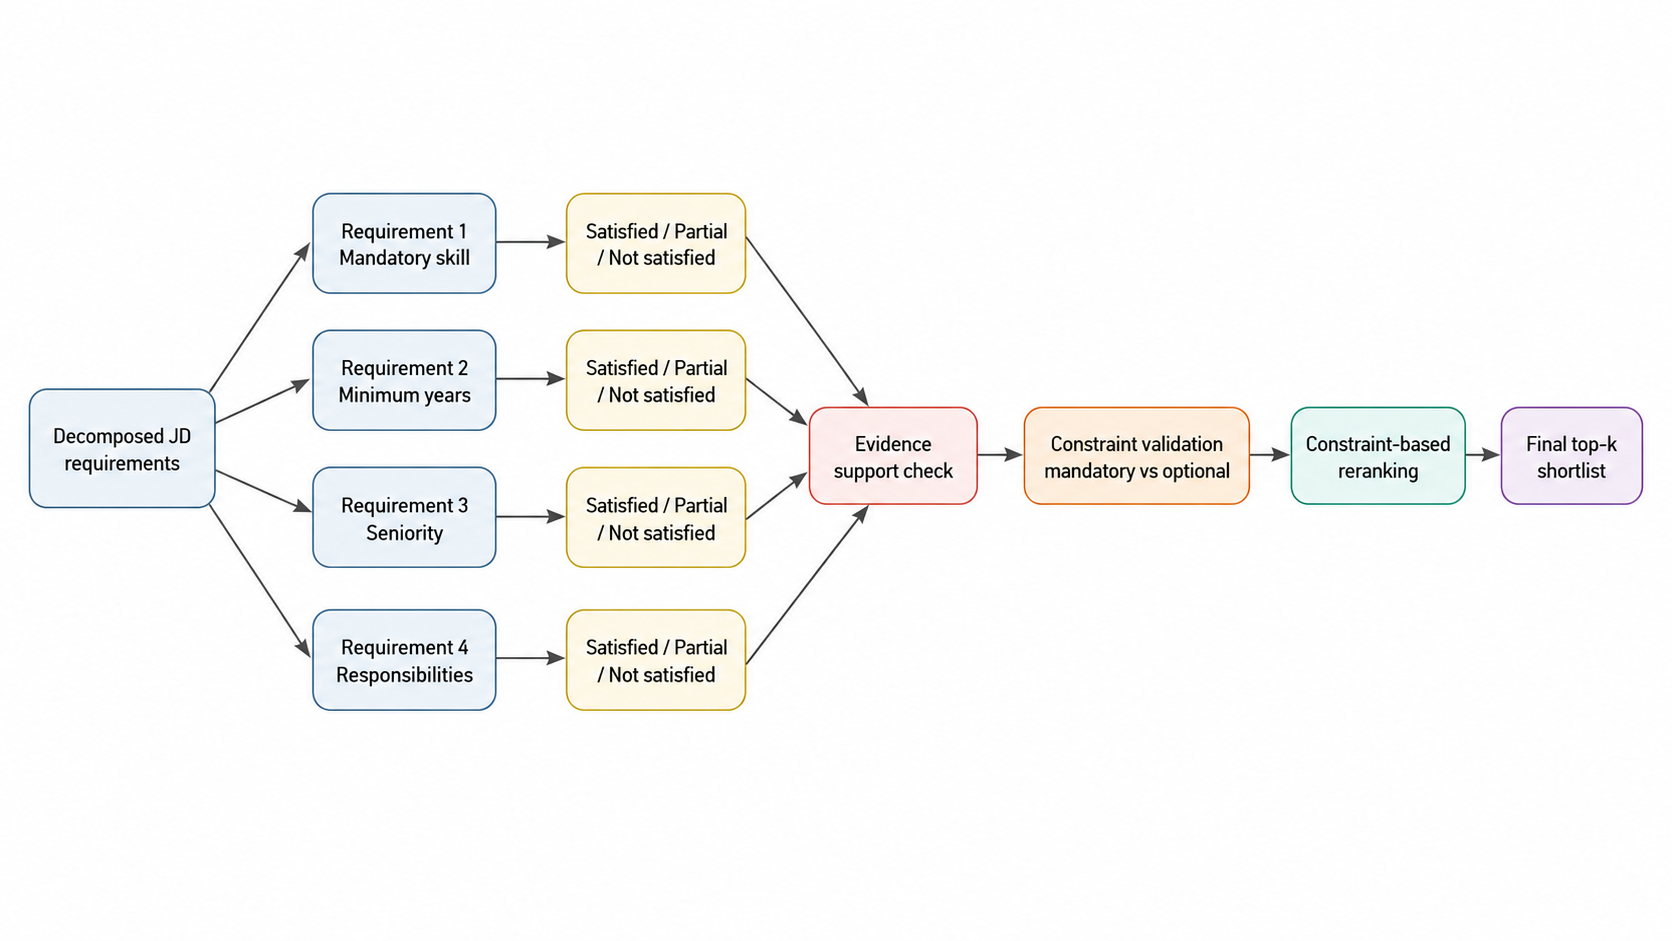
\includegraphics[width=0.98\textwidth]{figures/figure_3_7_requirement_level_assessment_and_constraint_based_reranking.png}
\caption{Requirement-level assessment and constraint-based reranking}
\label{fig:assessmentreranking}
\end{figure}

Each requirement receives one of four statuses:
\begin{table}[htbp]
\centering
\caption{Requirement satisfaction states}
\label{tab:states}
\begin{tabularx}{\textwidth}{>{\bfseries}p{0.23\textwidth}XX}
\toprule
Status & Definition & Example \\
\midrule
Satisfied & Requirement is explicitly supported by strong evidence & Spring Boot used in a production project \\
Partially satisfied & Related evidence exists but is incomplete or indirect & General cloud deployment but no AWS-specific evidence \\
Unsupported & Skill is declared but no supporting experience evidence is found & Kubernetes appears only in Skills \\
Not satisfied & Requirement is missing or contradicted & JD requires 5 years; CV shows 1 year \\
\bottomrule
\end{tabularx}
\end{table}

A configurable mapping converts these statuses to ordered values for deterministic reranking:
\begin{equation}
\rho(r_j,d)=
\begin{cases}
3, & \text{satisfied},\\
2, & \text{partially satisfied},\\
1, & \text{unsupported},\\
0, & \text{not satisfied}.
\end{cases}
\end{equation}

These values are not used as the research ground-truth labels. They are internal requirement states used by the mechanism.

\subsection{Operational Decision Rules}
To keep the implementation reproducible, the prototype applies explicit decision rules: exact skill evidence in Work Experience or Projects is satisfied; semantically related evidence above $\tau_h$ is also satisfied; evidence between $\tau_l$ and $\tau_h$ is partially satisfied; a skill found only in Skills is unsupported; and requirements with no declaration or evidence are not satisfied. The thresholds are configuration parameters, not universal constants; the current build leaves them at their initial defaults ($\tau_l{=}0.35$, $\tau_h{=}0.55$) rather than calibrating on a development subset, which \cref{sec:discussion} identifies as a likely cause of the ranking-effectiveness result (Table~\ref{tab:ranking-results}).

\begin{table}[htbp]
\centering
\caption{Operational requirement assessment rules}
\label{tab:assessment-rules}
\begin{tabularx}{\textwidth}{p{0.24\textwidth}Xp{0.22\textwidth}}
\toprule
Status & Operational rule & Prototype configuration \\
\midrule
Satisfied & Exact evidence or semantic evidence at or above the high threshold & $E_j \geq \tau_h$ \\
Partially satisfied & Related but incomplete evidence between the two thresholds & $\tau_l \leq E_j < \tau_h$ \\
Unsupported & Requirement term declared in Skills but no evidence in Experience or Projects & Declaration only \\
Not satisfied & No valid declaration/evidence, or an explicit constraint contradiction & $E_j < \tau_l$ \\
\bottomrule
\end{tabularx}
\end{table}

The final values of $\tau_l$ and $\tau_h$ are recorded with the experiment configuration. This prevents threshold selection from being hidden and is what makes the sensitivity analysis in Table~\ref{tab:threshold-sensitivity} reproducible.

\section{Experience and Seniority Validation}
Years of experience are extracted from explicit phrases and, where possible, employment date ranges. Seniority is mapped to the ordered scale:
\begin{equation}
\text{Intern} < \text{Fresher} < \text{Junior} < \text{Middle} < \text{Senior} < \text{Lead} < \text{Architect}.
\end{equation}

Experience-year alignment is defined as:
\begin{equation}
Y_{\mathrm{align}}(d,q)=\min\left(\frac{Y_d}{Y_q},1\right),
\end{equation}
where $Y_d$ is the candidate's estimated experience and $Y_q$ is the JD minimum. If no minimum is specified, the component is treated as not applicable.

Seniority-level alignment is defined using the ordinal distance $\Delta_L=L_q-L_d$:
\begin{equation}
L_{\mathrm{align}}(d,q)=
\begin{cases}
1.0, & \Delta_L \leq 0,\\
0.5, & \Delta_L = 1,\\
0.0, & \Delta_L \geq 2.
\end{cases}
\end{equation}
The combined alignment is:
\begin{equation}
S_{\mathrm{align}}(d,q)=\frac{Y_{\mathrm{align}}(d,q)+L_{\mathrm{align}}(d,q)}{2}.
\end{equation}
A CV with no detectable year phrase or date range is currently recorded as 0.0 years, indistinguishable from a genuine 0-years fresher (see Limitations, Chapter 5). Roughly 20\% of indexed real CVs (598/2,986) show 0.0 years -- plausibly a mix of both cases, worth spot-checking during the manual "Experience-year correctness" inspection (Table~\ref{tab:ocr-results}).

\section{Constraint-based Reranking}
The proposed method does not calculate one weighted final similarity score. Candidates are ordered by a lexicographic ranking key:
\begin{equation}
K(d,q)=\left(H_{\mathrm{pass}},C_h,E_h,S_{\mathrm{align}},C_s,E_s,B\right),
\label{eq:ranking-key}
\end{equation}
where the components are defined in Table~\ref{tab:ranking-components}.

\begin{table}[htbp]
\centering
\caption{Definition of constraint-based reranking components}
\label{tab:ranking-components}
\begin{tabularx}{\textwidth}{>{\bfseries}p{0.15\textwidth}X}
\toprule
Component & Operational definition \\
\midrule
$H_{\mathrm{pass}}$ & 1 when no hard requirement is not satisfied; otherwise 0. \\
$C_h$ & Sum of normalized satisfaction values for hard requirements divided by the number of hard requirements. \\
$E_h$ & Number of hard requirements with valid Experience/Project evidence divided by the number of hard requirements. \\
$S_{\mathrm{align}}$ & Mean of experience-year and seniority-level alignment. \\
$C_s$ & Sum of normalized satisfaction values for soft requirements divided by the number of soft requirements. \\
$E_s$ & Number of soft requirements with valid supporting evidence divided by the number of soft requirements. \\
$B$ & SBERT full-document similarity used only as the final tie-breaker. \\
\bottomrule
\end{tabularx}
\end{table}

The requirement-state mapping $\rho\in\{0,1,2,3\}$ is normalized by dividing by three before coverage calculation. Empty hard- or soft-requirement groups are handled by neutral defaults documented in the experiment configuration. Candidates are sorted lexicographically in descending order. Consequently, a candidate who passes all hard constraints is prioritized over one who fails a hard constraint, even when the latter has higher broad semantic similarity.

\subsection{Reranking Procedure}
\begin{lstlisting}[basicstyle=\ttfamily\small,frame=single,breaklines=true,caption={Requirement-aware and evidence-aware reranking procedure},label={alg:reranking}]
Input: job description q, CV corpus D, top-k value k
Output: ranked candidates with explanations

1. Parse q into hard requirements Rh and soft requirements Rs.
2. For each CV d in D:
3.     Parse CV sections and extraction-quality metadata.
4.     Extract candidate experience years and seniority.
5.     For each requirement r in Rh union Rs:
6.         Retrieve the highest-similarity evidence sentence.
7.         Assign satisfied, partial, unsupported, or not-satisfied status.
8.     Validate hard requirements and calculate Hpass.
9.     Calculate Ch, Eh, Salign, Cs, Es, and baseline score B.
10.    Build ranking key K(d,q).
11. Sort candidates lexicographically by K(d,q), descending.
12. Return the top-k candidates and requirement-level explanations.
\end{lstlisting}

\Cref{fig:app-ranking} shows the Ranking tab after running the full proposed model (M6) against a JD with at least one hard requirement most candidates cannot satisfy, producing a mix of \emph{Hard pass} and \emph{Constraint gap} badges. It is the single screenshot that most directly demonstrates constraint-based reranking (\cref{eq:ranking-key}): a candidate must not out-rank a hard-pass candidate purely on broad similarity.

\begin{figure}[htbp]
\centering
\appscreenshot{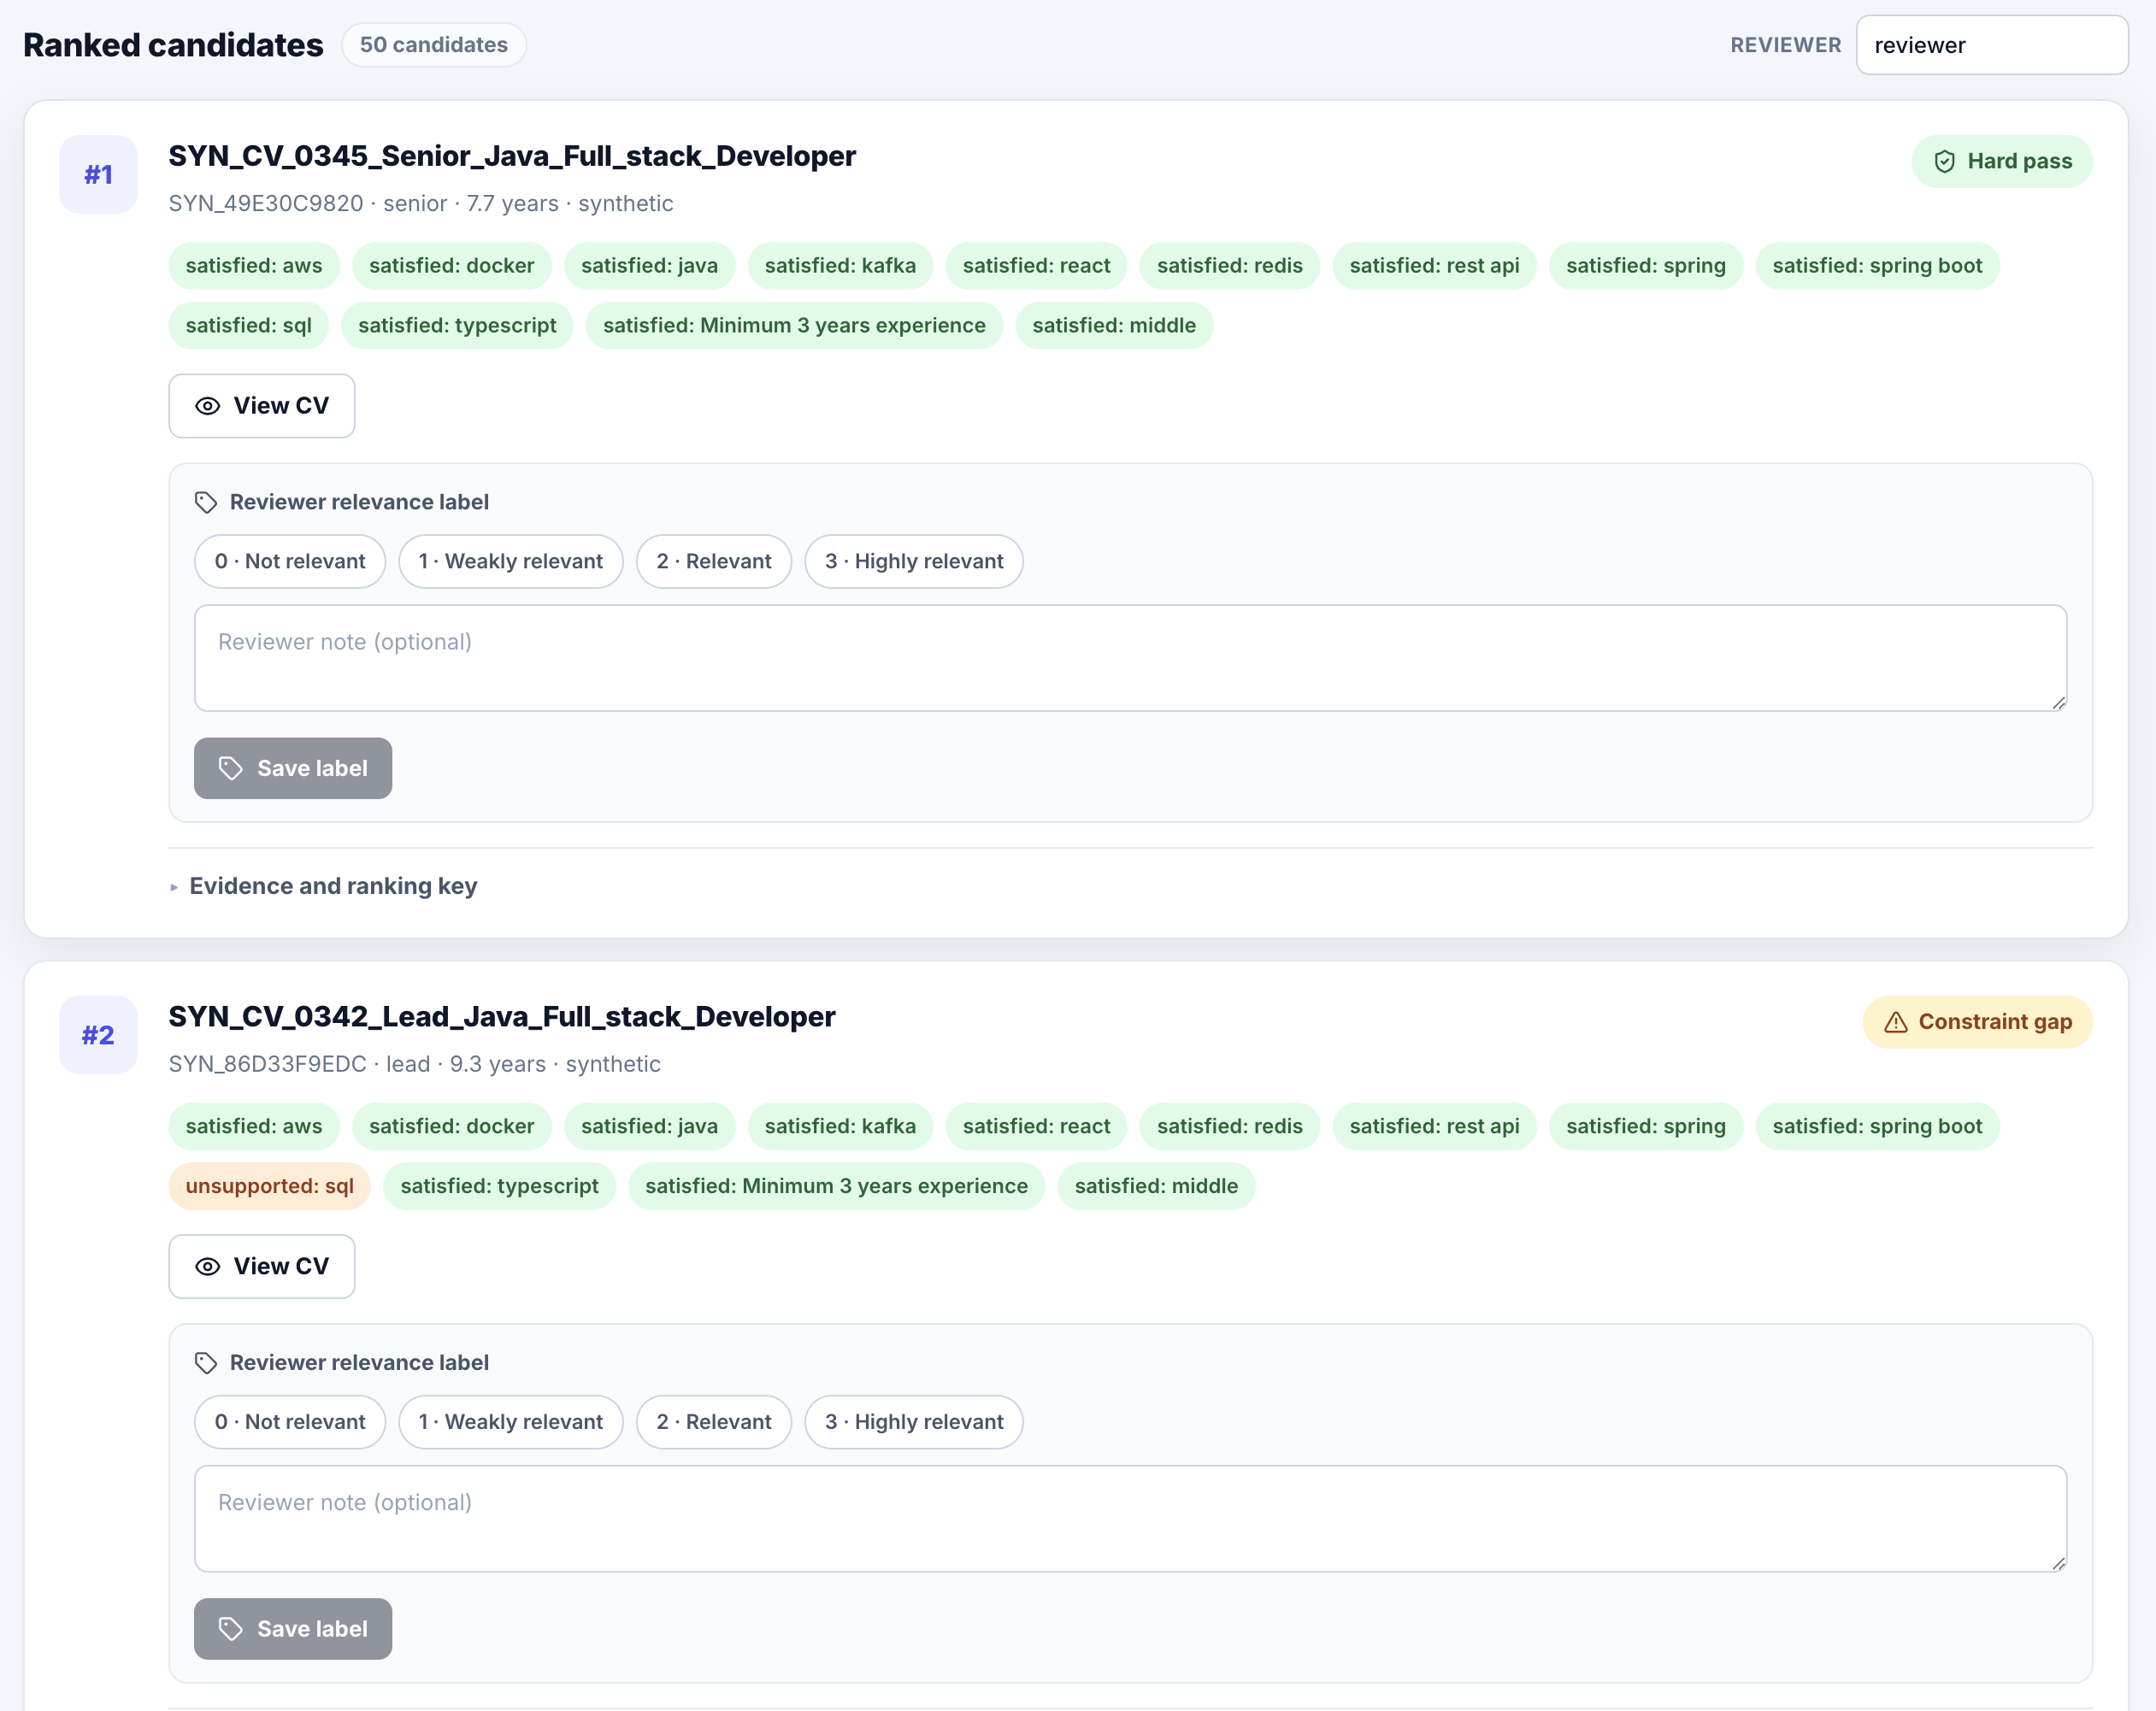
\includegraphics[width=0.92\textwidth]{figures/figure_3_8_topk_ranking_results.png}}
\caption{Top-$k$ ranking results}
\label{fig:app-ranking}
\end{figure}

\section{Baseline Methods}
The following baselines are retained for comparison:
\begin{enumerate}
  \item \textbf{TF--IDF full text}: lexical cosine similarity.
  \item \textbf{SBERT full text}: full-document semantic similarity.
  \item \textbf{Section-level SBERT}: separate similarity for Skills, Experience, Education, and overall text.
  \item \textbf{Requirement-aware}: requirement decomposition and coverage without evidence verification.
  \item \textbf{Requirement + seniority constraints}: adds hard-constraint gating and the lexicographic key on top of requirement-aware coverage, still without semantic evidence verification.
  \item \textbf{Full proposed model}: requirement-aware, evidence-aware, seniority-aware, constraint-based reranking.
\end{enumerate}

\section{Explanation Generation}
For each candidate, the explanation page displays:
\begin{itemize}
  \item hard constraints passed and violated;
  \item satisfied, partially satisfied, unsupported, and missing requirements;
  \item required and candidate experience years;
  \item required and candidate seniority;
  \item supporting evidence sentences;
  \item OCR or parsing warnings;

  \item reviewer relevance label and note.
\end{itemize}

\Cref{fig:app-explanation} shows the CV viewer modal for one ranked candidate, with the left evidence panel -- rank, hard-constraint status, per-requirement assessment list with evidence sentences, and the raw ranking key -- next to the embedded PDF. The candidate shown has at least one \emph{satisfied}, one \emph{partially satisfied}, and one \emph{unsupported} or \emph{not satisfied} requirement, so all four states from Table~\ref{tab:states} appear together in a single view.

\begin{figure}[htbp]
\centering
\appscreenshot{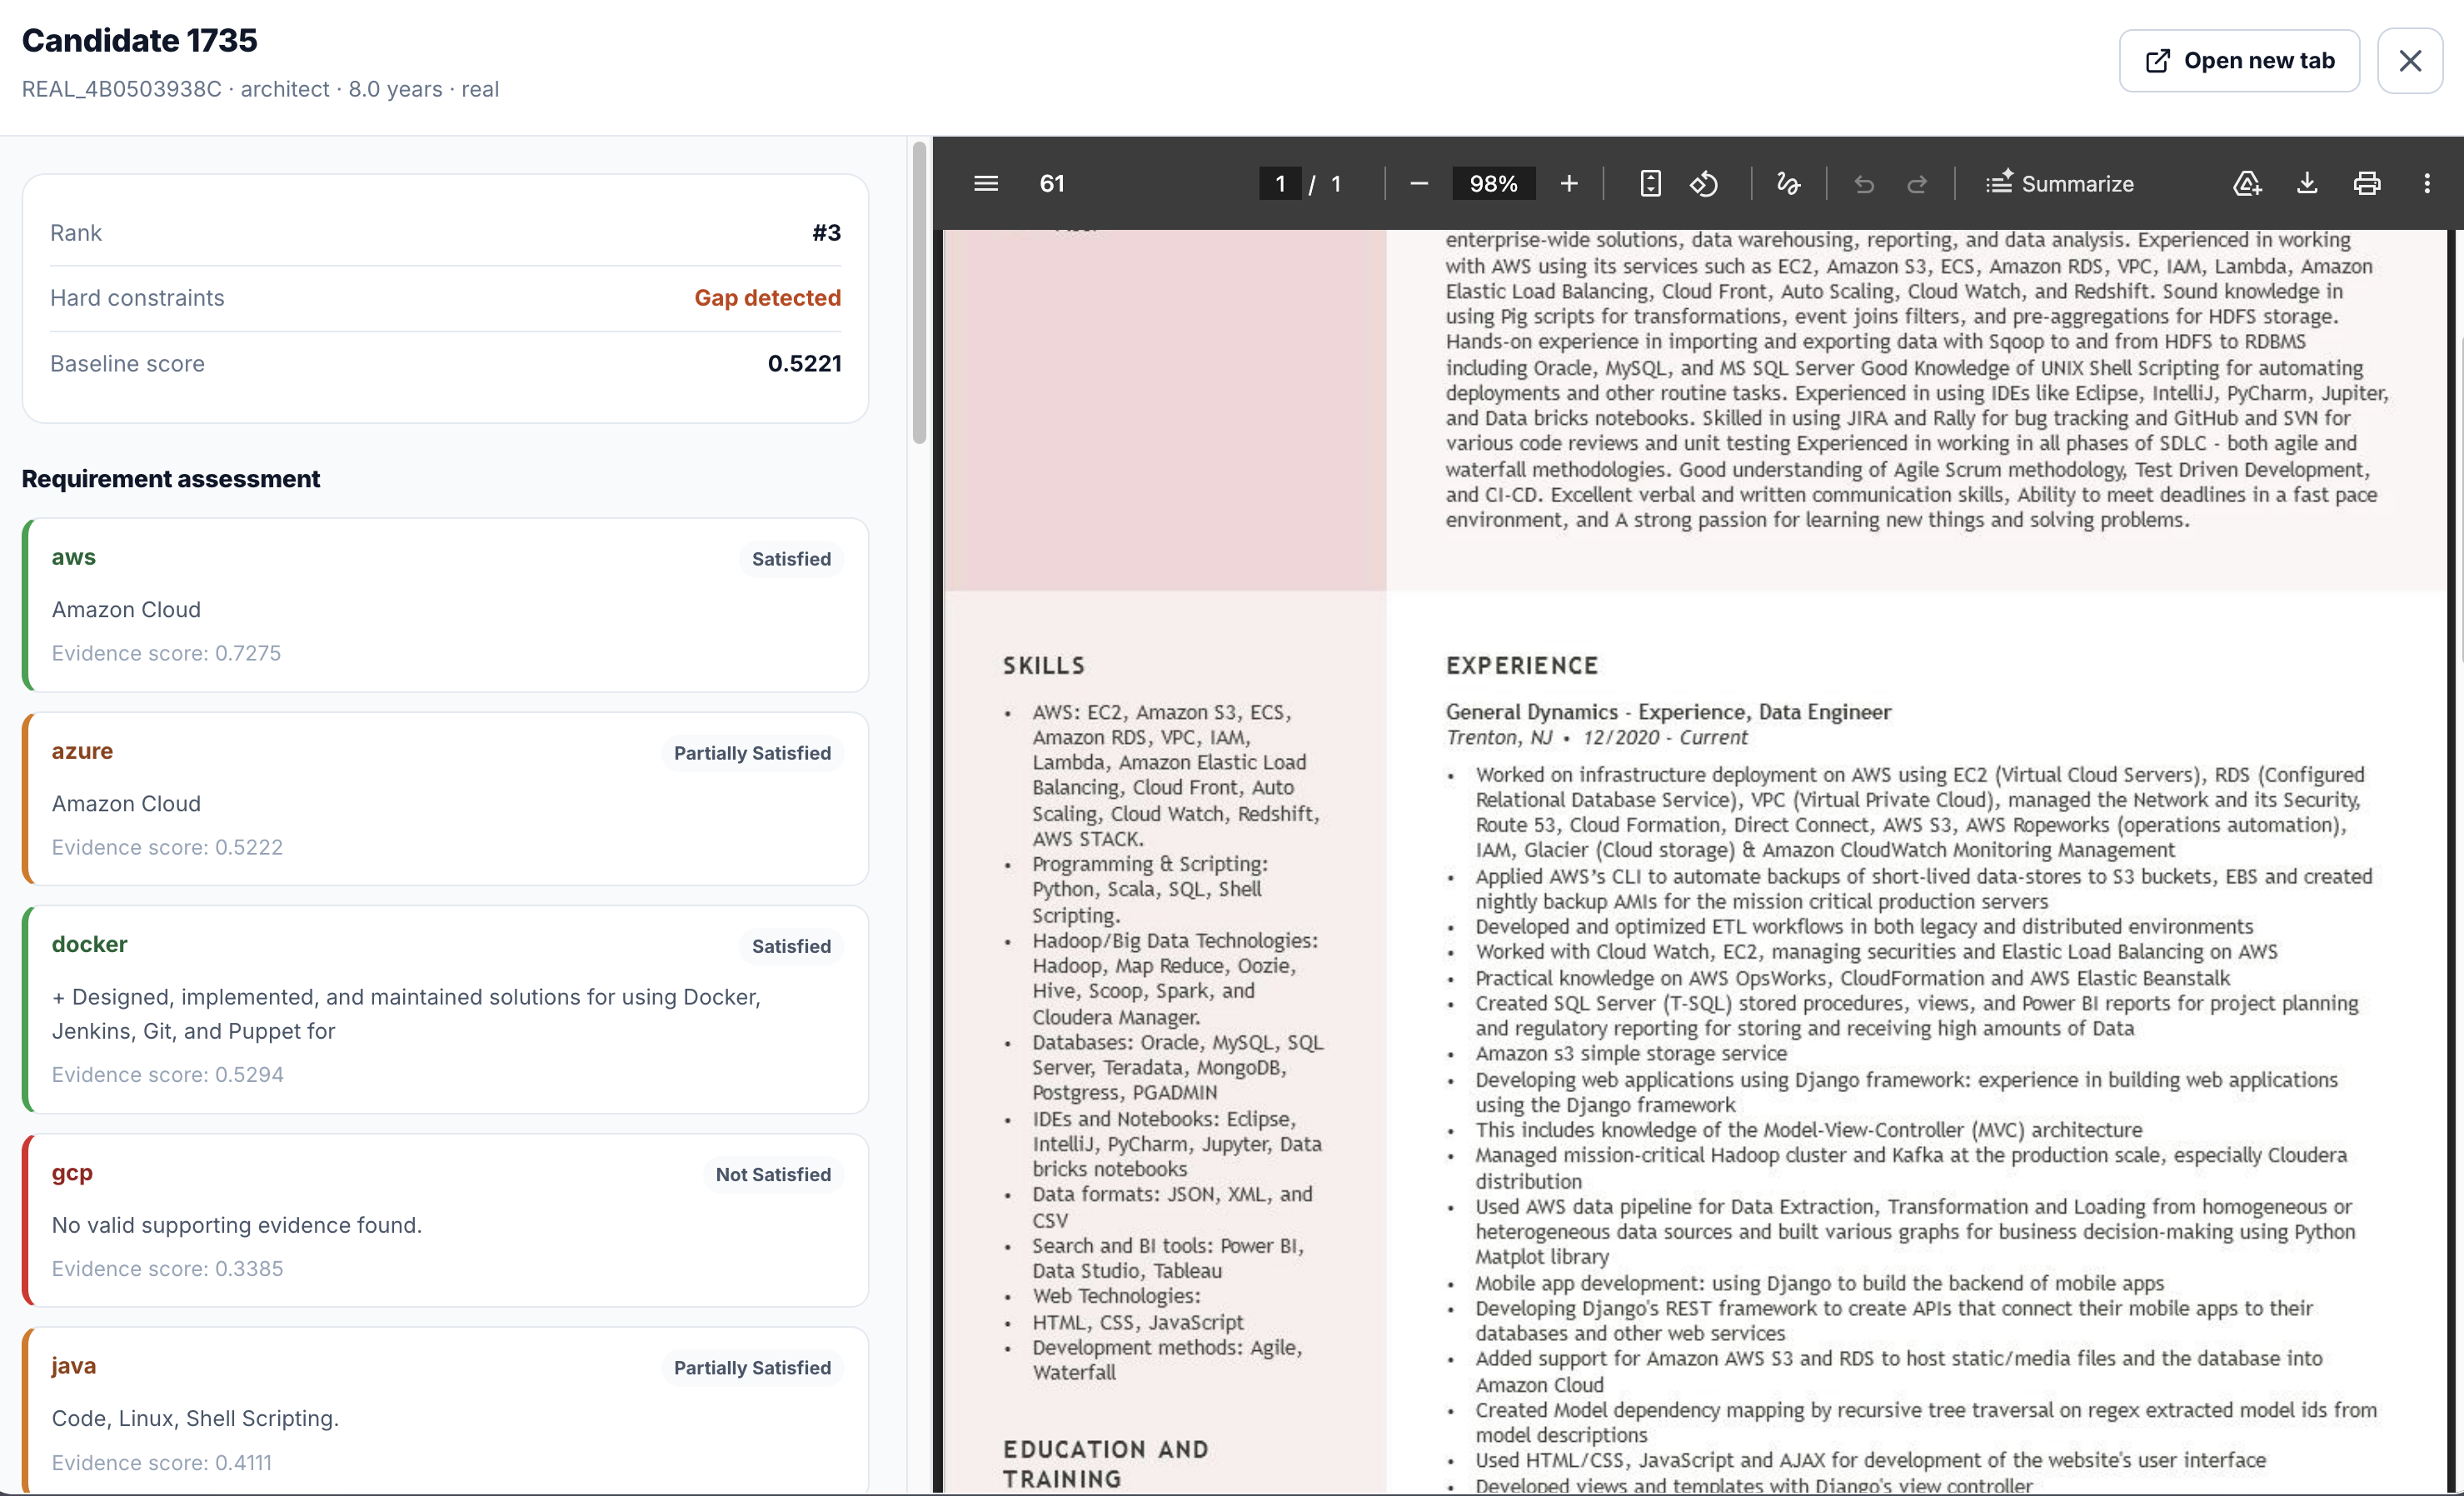
\includegraphics[width=0.92\textwidth]{figures/figure_3_9_candidate_requirement_explanation.png}}
\caption{Candidate requirement-level explanation}
\label{fig:app-explanation}
\end{figure}

\begin{figure}[htbp]
\centering
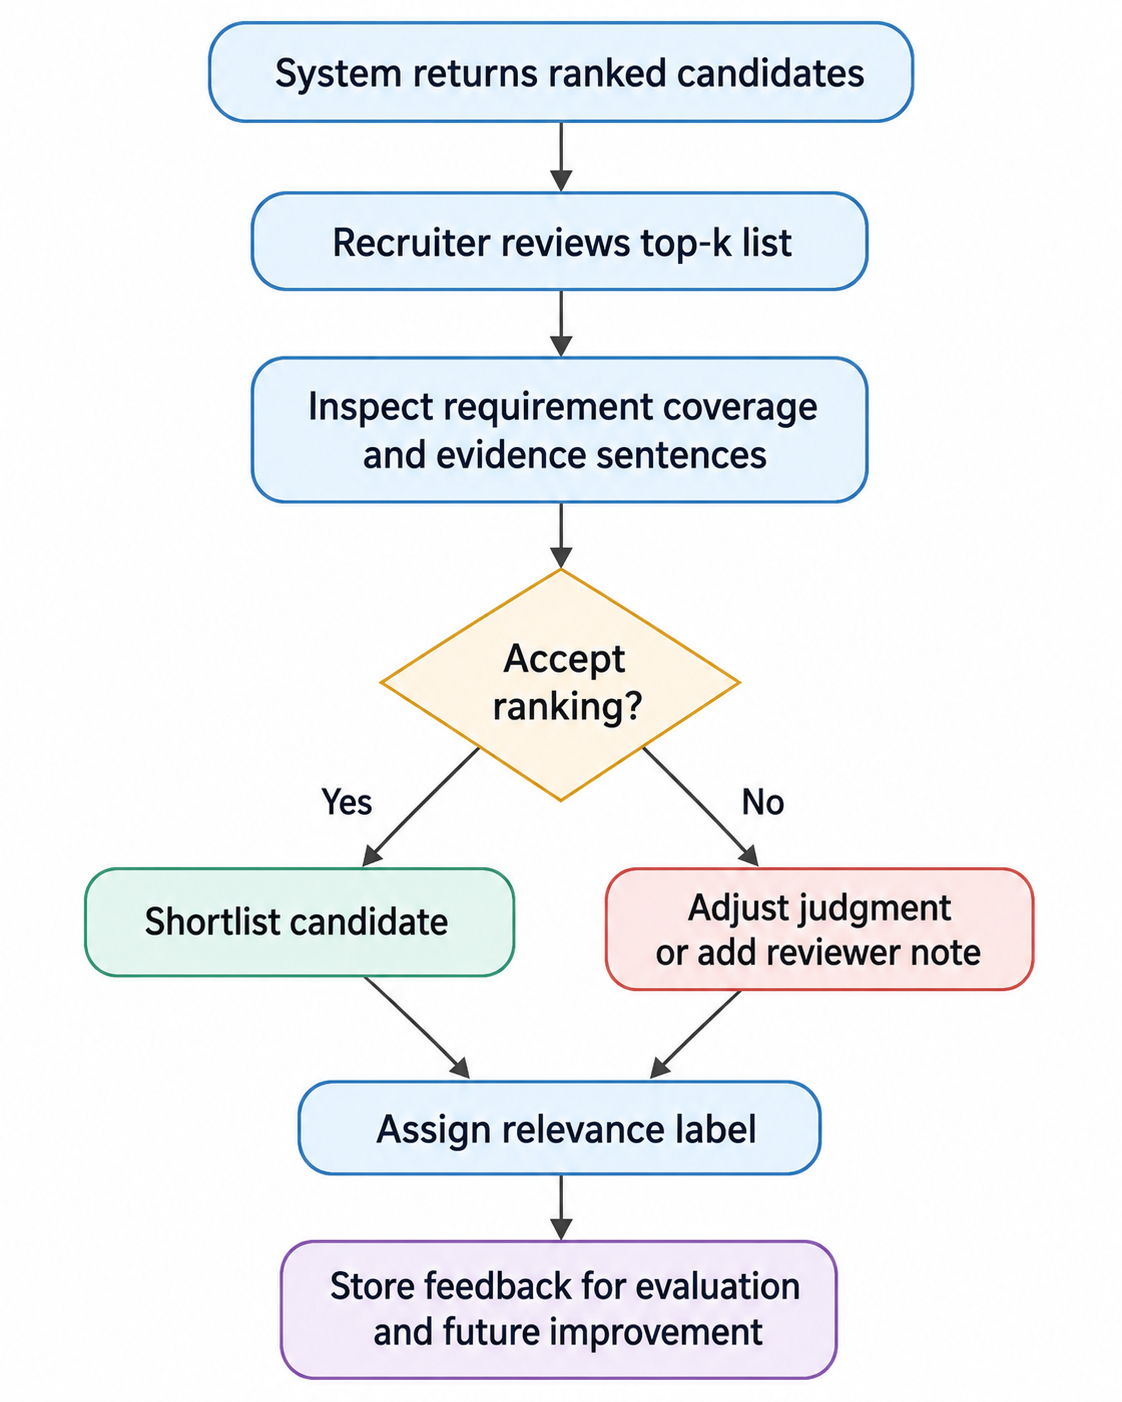
\includegraphics[height=0.68\textheight,keepaspectratio]{figures/figure_3_10_human_in_the_loop_recruiter_review_workflow.png}
\caption{Human-in-the-loop recruiter review workflow}
\label{fig:reviewworkflow}
\end{figure}

\section{Software Architecture}
\label{sec:architecture-impl}
The backend is implemented with Python and FastAPI. PyPDF handles text-based PDF extraction, while pdf2image and Tesseract provide OCR fallback. Scikit-learn implements TF--IDF. Sentence-transformers provides SBERT embeddings. SQLite is sufficient for the prototype; PostgreSQL and FAISS are deployment options for larger corpora. The frontend is implemented in ReactJS.

Each CV's SBERT embeddings (full-document, per-section, per-evidence-sentence) are computed once and cached in memory, keyed by CV id and guarded by a content hash so a changed record never serves a stale vector. Ranking against a new JD therefore only re-embeds the JD's short query text; the CV corpus is embedded once per process lifetime, not per ranking call. This is why the operational-performance figures (Table~\ref{tab:performance-results}) show a one-time index-build cost far larger than the marginal per-JD ranking cost. To keep that one-time cost off the critical path of the first user-triggered ranking call -- important during a live demo, where minutes of silence could look like a hang -- the backend pre-warms the cache for every indexed CV in a background thread at server startup.

\begin{table}[htbp]
\centering
\caption{Implementation and experiment environment}
\label{tab:environment}
\begin{tabularx}{\textwidth}{p{0.31\textwidth}X}
\toprule
Item & Recorded configuration \\
\midrule
Backend runtime & Python 3.12.5; FastAPI 0.115.6; Uvicorn 0.34.0; SQLAlchemy 2.0.36 \\
Frontend runtime & Node.js 23.7.0; React 18.3.1 \\
Embedding library/model & sentence-transformers 3.3.1, checkpoint \texttt{all-MiniLM-L6-v2} (384-dim); PyTorch 2.2.2; NumPy 1.26.4; SciPy 1.13.1; scikit-learn 1.6.0 \\
PDF/OCR stack & PyPDF 5.1.0; pdf2image 1.17.0; Tesseract 5.5.2; Poppler (\texttt{pdftoppm}) 26.07.0 \\
Storage & SQLite prototype database (single file) \\
Execution hardware & Intel x86\_64, macOS 15.4.1, 12 logical CPUs, 16\,GB RAM; CPU-only, no GPU; a personal dev machine with ordinary background load (browser, IDE), not an isolated benchmarking rig -- latency figures in Table~\ref{tab:performance-results} shifted roughly $2$--$3\times$ between measurement passes under different load, hence the reported ranges rather than single calls \\
Randomness & The ranking mechanism is deterministic given fixed embeddings and thresholds; the labeled pool's candidate-pooling step (\cref{sec:labeled-pool}) used a supplementary random sample with no recorded seed, so it cannot be regenerated exactly (Limitations, Chapter 5) -- the $\tau$-calibration dev/test split (\cref{sec:calibration}), by contrast, used a fixed seed \\
\bottomrule
\end{tabularx}
\end{table}

These fields are separated from the algorithm description so the final experiment can be reproduced without changing the proposed mechanism.

\begin{table}[htbp]
\centering
\caption{Main software modules}
\label{tab:modules}
\begin{tabularx}{\textwidth}{>{\bfseries}p{0.28\textwidth}X}
\toprule
Module & Responsibility \\
\midrule
PDF ingestion & Validation, direct extraction, OCR fallback, quality flags \\
Preprocessing & Text cleaning and normalization; content-hash duplicate detection at ingestion; PII masking is not implemented (Chapter 5, Limitations) \\
CV parser & Section extraction, sentence segmentation, skills, dates \\
JD parser & Mandatory/optional requirements, responsibilities, education, certifications, years, seniority \\
Evidence retriever & Requirement-to-sentence semantic matching, with a per-CV embedding cache for repeat ranking calls \\
Constraint engine & Hard/soft validation and seniority checks \\
Reranking engine & Lexicographic requirement-based ordering; M1--M6 baseline catalogue selectable per call \\
Explanation service & Requirement states, evidence, gaps, warnings \\
Dataset provenance service & Source type and extraction status are implemented; scenario metadata and experiment split are designed but not yet implemented \\
Evaluation service & Reviewer labels (with a labeling UI) and NDCG/MAP/MRR/Recall metrics per baseline are implemented; robustness-set construction, latency benchmarking, and the usability pilot are evaluation activities the researcher runs using these outputs, not automated in-app pipelines \\
\bottomrule
\end{tabularx}
\end{table}

\section{API Design}
\begin{table}[htbp]
\centering
\caption{Main API endpoints}
\label{tab:api}
\begin{tabularx}{\textwidth}{p{0.35\textwidth}p{0.12\textwidth}X}
\toprule
Endpoint & Method & Purpose \\
\midrule
\texttt{/api/\allowbreak health} & GET & Health check; also reports the active $\tau_l$/$\tau_h$ evidence thresholds \\
\texttt{/api/\allowbreak cvs/\allowbreak upload-pdfs} & POST & Upload PDF CVs, extract text, apply OCR fallback, and index valid records \\
\texttt{/api/\allowbreak cvs} & GET & List indexed CV profiles and parsing status \\
\texttt{/api/\allowbreak jds} & POST & Create a JD from an explicit requirement list \\
\texttt{/api/\allowbreak jds/\allowbreak upload-pdfs} & POST & Create JD(s) from PDF, auto-decomposed into mandatory/optional skills, responsibilities, education, and certifications \\
\texttt{/api/\allowbreak jds/\allowbreak \{id\}} & GET & Retrieve a JD, including its decomposed requirements \\
\texttt{/api/\allowbreak jds/\allowbreak \{id\}/\allowbreak rank} & POST & Run one baseline from the M1--M6 catalogue (\texttt{method} query parameter) or the full proposed mechanism (default); requirement-level assessments are returned inline per candidate rather than through a separate explanation endpoint \\
\texttt{/api/\allowbreak labels} & POST & Save a reviewer relevance label (0--3) and note for a CV--JD pair \\
\texttt{/api/\allowbreak jds/\allowbreak \{id\}/\allowbreak labels} & GET & Retrieve saved reviewer labels for a JD \\
\texttt{/api/\allowbreak experiments/\allowbreak methods} & GET & List the M1--M6 baseline catalogue \\
\texttt{/api/\allowbreak jds/\allowbreak \{id\}/\allowbreak experiments/\allowbreak compare} & POST & Run every M1--M6 baseline against the same CV pool and score each against saved reviewer labels \\
\texttt{/api/\allowbreak experiments/\allowbreak \{id\}/\allowbreak metrics} & GET & Return NDCG/MAP/MRR/Recall for the full model against saved labels \\
\bottomrule
\end{tabularx}
\end{table}

\section{Security and Human-in-the-loop Controls}
\label{sec:security}
File types are validated (PDF only); explicit file-size limits are not yet enforced. Raw CV content is not sent to external APIs in the local prototype -- OCR (Tesseract) and embedding (sentence-transformers) both run locally. The system does not automatically reject candidates from ranking based on suitability. Recruiters remain responsible for final screening and hiring decisions.

Direct identifiers (names, emails, phone numbers, addresses) are not masked before ranking: \texttt{clean\_text} and the original PDF both retain the candidate's contact details, so this is listed as a limitation rather than a delivered control (Chapter 5). Content-based duplicate detection runs at ingestion: a SHA-256 hash of the normalized text is compared against already-indexed CVs, so re-uploading the same PDF is rejected as \texttt{duplicate\_content} rather than silently indexed twice.

% ==================================================
\chapter{Evaluation and Discussion}
% ==================================================

\section{Evaluation Goals}
The evaluation is designed to answer whether the proposed mechanism improves CV--JD matching rather than merely producing a score. It measures:
\begin{itemize}
  \item ranking effectiveness;
  \item reduction of seniority-mismatch false positives;
  \item resistance to keyword stuffing and unsupported skill claims;
  \item PDF extraction and OCR reliability;
  \item explanation usefulness and error characteristics.
\end{itemize}


\begin{figure}[htbp]
\centering
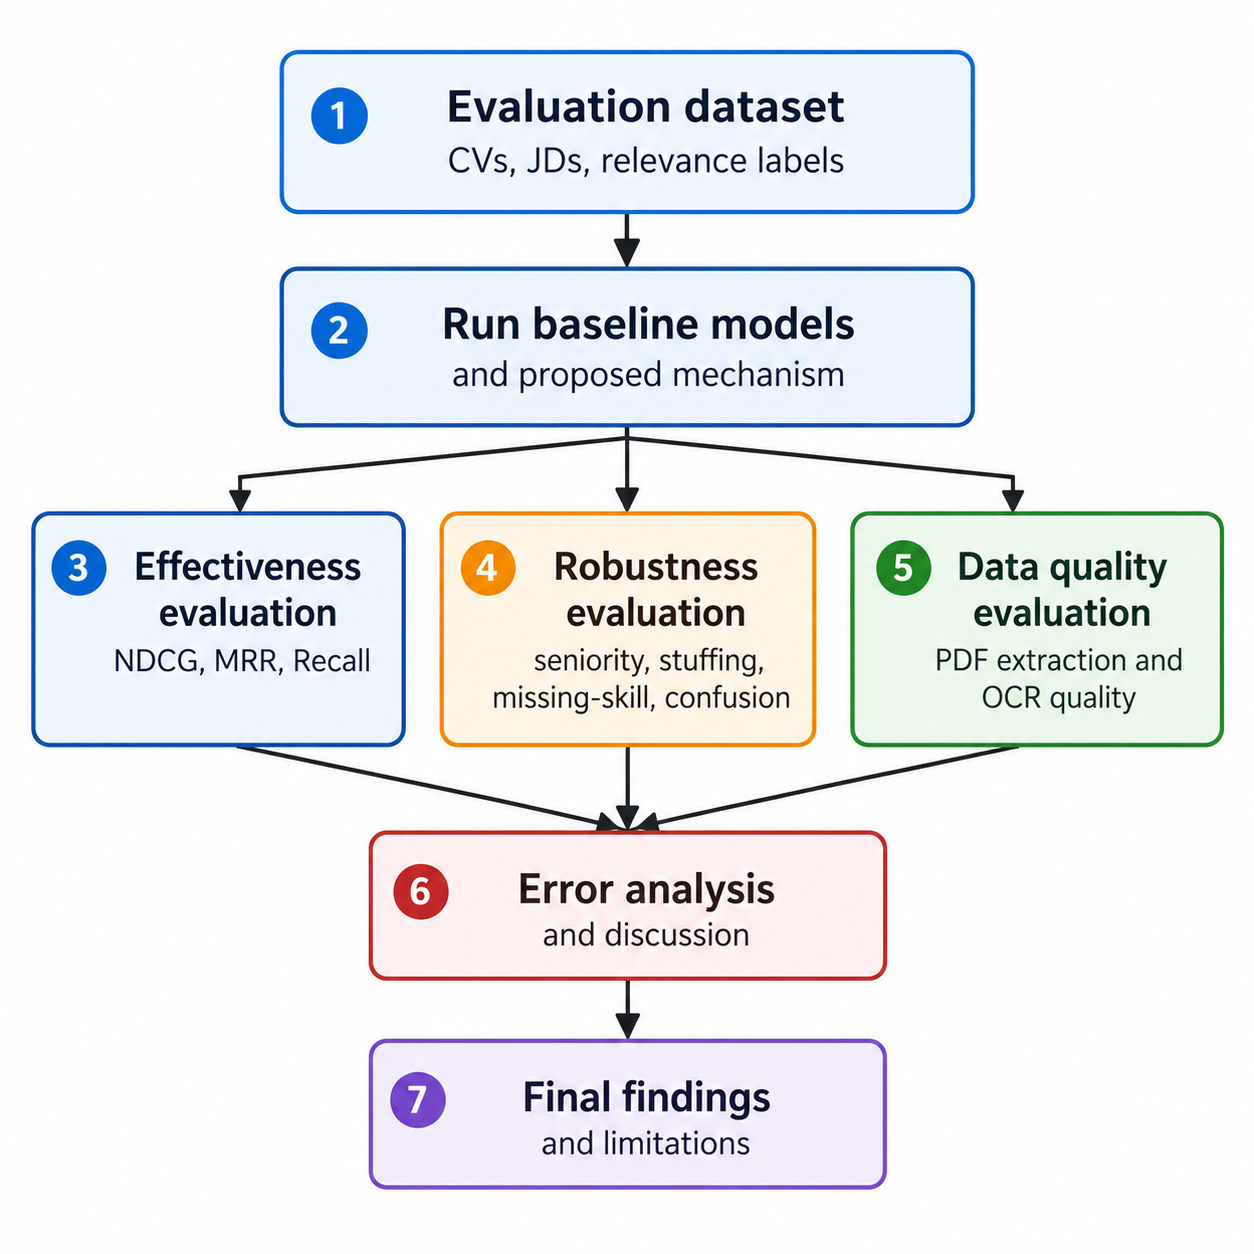
\includegraphics[width=0.85\textwidth,keepaspectratio]{figures/figure_4_1_evaluation_workflow_for_effectiveness_robustness_and_data_quality.png}
\caption{Evaluation workflow for effectiveness, robustness, and data quality}
\label{fig:evaluationworkflow}
\end{figure}

\section{Dataset and Test Corpus}
The evaluation corpus is split into distinct subsets so that real-world effectiveness, controlled robustness, and scalability are not conflated. Current indexed sizes are in Table~\ref{tab:dataset-composition}; dataset name, URL, and license are in Table~\ref{tab:dataset-fields}. Raw pre-filter counts remain \texttt{Pending external input} until the final corpus audit.

\subsection{Real Scanned PDF Corpus}
The source Kaggle dataset \emph{Resume Dataset PDF} \citep{hadikpresumepdf} (CC0: Public Domain) is a general resume collection spanning many professions, not just IT. Since this thesis's ranking mechanism, requirement dictionary, and evaluation JDs are scoped to IT/software recruitment, only IT/software-relevant resumes were retained on import; CVs from unrelated professions were excluded and never entered the running prototype. The real corpus currently holds 2,986 scanned resume PDFs after this filtering (subject to change after a final corpus audit and duplicate removal). Because records are image-based, OCR is required before parsing. The final report will additionally record the original pre-filter count, English-language count, IT-domain count, duplicate-removal count, and OCR success/failure counts -- none of which the current pipeline logs retroactively (\cref{sec:limitations-list}).

The real corpus is used for:
\begin{itemize}
  \item OCR and document-ingestion evaluation;
  \item section, skill, experience, and seniority parsing analysis;
  \item human-labeled CV--JD ranking evaluation;
  \item real-world case studies and error analysis.
\end{itemize}

\subsection{Controlled Synthetic CV Corpus}
Approximately 1,000 AI-generated English IT CVs expand corpus size and create controlled combinations of role, seniority, years, responsibilities, evidenced skills, unsupported claims, and irrelevant skills. They are used for the dedicated robustness and scalability sets, but not confined to them: 108 of the 246 candidates in the primary human-labeled pool are also synthetic (\cref{sec:labeled-pool}), so synthetic data feeds Table~\ref{tab:ranking-results} directly, not only the robustness tables. Real CVs remain the majority (56.1\%) of that pool, so synthetic data is not the sole evidence of practical effectiveness.

Each synthetic record carries a manifest of role, seniority, years of experience, declared/evidenced/unsupported skills, responsibility profile, scenario type, prompt version, and QC status. The final model name, prompt template, role/seniority distribution, and accepted/rejected counts remain \texttt{Pending external input}.

\subsection{Combined Retrieval Corpus}
The combined retrieval corpus holds all valid real and accepted synthetic CVs -- currently 3,986 records (2,986 real, 1,000 synthetic) -- and is used to measure indexing time, ranking latency, and top-$k$ response time (Table~\ref{tab:performance-results}). The human-labeled pool mixes both sources rather than separating them (138 real, 108 synthetic of the 246 pairs, \cref{sec:labeled-pool}), and Table~\ref{tab:ranking-results} reports one combined macro-average over that mixed pool; a separate real-only/synthetic-only breakdown was not performed and is noted as a gap in \cref{sec:limitations-list}.

\subsection{Human-labeled Evaluation Pool}
\label{sec:labeled-pool}
The primary ranking evaluation uses a manually judged pool of CV--JD pairs, labeled for five representative IT JDs (EVAL\_JD\_01--05; Table~\ref{tab:dataset-fields}) and drawn from both the real and synthetic corpora. The final 246-pair pool is 138 real (56.1\%) and 108 synthetic (43.9\%) CVs -- within the planned 150--250-pair range, though the real/synthetic split itself was not a pre-registered target.

Candidate pooling combined the top results from all six models (TF--IDF, SBERT full text, section-level SBERT, requirement-aware, requirement+seniority, full proposed model) plus a supplementary random sample per JD, to avoid bias toward any single model's top-$k$; duplicates were removed before judgment. The one-time random-sampling step used no recorded seed, so that draw cannot be regenerated exactly -- but the resulting 246 labeled pairs are stored and are what all six methods in Table~\ref{tab:ranking-results} are scored against, so the ground truth itself is fully reproducible even though the original pooling draw is not (see Limitations, Chapter 5).

\subsection{Controlled Robustness Sets}
\label{sec:robustness-sets}
Separate controlled sets are constructed for:
\begin{itemize}
  \item seniority mismatch: same or similar technology stack with different experience and ownership levels;
  \item keyword stuffing: skills added to the Skills section without supporting evidence;
  \item supported skill addition: skills added together with relevant Experience or Project evidence;
  \item missing mandatory requirement: strong broad similarity but one or more hard requirements absent;
  \item role confusion: related IT roles with overlapping terminology but different responsibilities.
\end{itemize}

\begin{table}[htbp]
\centering
\caption{Dataset composition for the final experiment}
\label{tab:dataset-composition}
\begin{tabularx}{\textwidth}{>{\bfseries}p{0.25\textwidth}p{0.18\textwidth}p{0.17\textwidth}X}
\toprule
Subset & Source & Final size & Primary purpose \\
\midrule
Real scanned PDF corpus & Kaggle & 2,986 indexed (100\% of \emph{indexed} records OCR-extracted by construction -- files that failed OCR are not indexed and are excluded from this denominator; raw pre-filter count \texttt{Pending}) & OCR, parsing, ranking, and error analysis \\
Synthetic CV corpus & AI-generated & 1,000 & Controlled robustness and scalability \\
Combined retrieval corpus & Mixed & 3,986 & Indexing and ranking latency \\
Human-labeled evaluation pool & Real + synthetic CVs, single reviewer (138 real, 108 synthetic) & 246 labeled pairs across the 5 EVAL\_JD JDs (46--50 each; target 150--250 met) & NDCG, MAP, MRR, Recall (Table~\ref{tab:ranking-results}) \\
Seniority robustness set & Purpose-built synthetic pairs & 3 pairs, 3 JDs (Java, React, data engineer) & Hard-constraint violation analysis (Tables~\ref{tab:robustness-results}, \ref{tab:battery-summary}); all 5 declared categories built, \cref{sec:robustness-sets} \\
Keyword-stuffing set & Controlled paired variants & 3 triples, 3 JDs (EVAL\_JD\_01, Vue, data engineer) & Unsupported-claim and rank-change analysis (Tables~\ref{tab:robustness-results}, \ref{tab:battery-summary}) \\
Missing-mandatory-requirement set & Purpose-built synthetic pairs & 3 pairs, 3 JDs (Python, DevOps, QA) & Broad-similarity-vs-hard-gate analysis (Tables~\ref{tab:missing-mandatory-case}, \ref{tab:battery-summary}) \\
Role-confusion set & Purpose-built synthetic pairs & 3 pairs, 3 JDs (Java, data, DevOps) & Requirement-level role discrimination vs.\ confused PM/BA/QA tester (Tables~\ref{tab:role-confusion-case}, \ref{tab:battery-summary}) \\
\bottomrule
\end{tabularx}
\end{table}

Summing every row above (2,986 real $+$ 1,000 synthetic $+$ 27 robustness-battery CVs: 6 seniority, 9 stuffing, 6 missing-mandatory, 6 role-confusion) gives the full 4,013 CV records held in the running prototype after the final battery expansion. The 3,986-CV ``combined retrieval corpus'' used for effectiveness (Table~\ref{tab:ranking-results}) and performance (Table~\ref{tab:performance-results}) deliberately excludes the 27 robustness-battery CVs, since those are purpose-built single-JD/single-pair fixtures rather than participants in the macro-averaged measurements. The rank-based robustness and case-study tables (Tables~\ref{tab:robustness-results}--\ref{tab:role-confusion-case}) were all re-run against the full 4,013-CV corpus so their rank denominators agree; the one exception is the threshold-sensitivity table (\cref{sec:calibration}), which re-runs the full 246-pair NDCG/MAP evaluation rather than single-CV ranks and was left at an earlier 3,991-CV snapshot.

\Cref{fig:dataset-chart} visualizes this composition: the left chart shows the 3,986-CV combined retrieval corpus as 74.9\% real scanned PDFs and 25.1\% synthetic AI-generated CVs, while the right chart shows the 246-pair human-labeled evaluation pool is itself a mix of both sources -- 56.1\% (138) real and 43.9\% (108) synthetic, drawn from 5 evaluation JDs at 46--50 labeled candidates each -- not an all-real subset.

\begin{figure}[htbp]
\centering
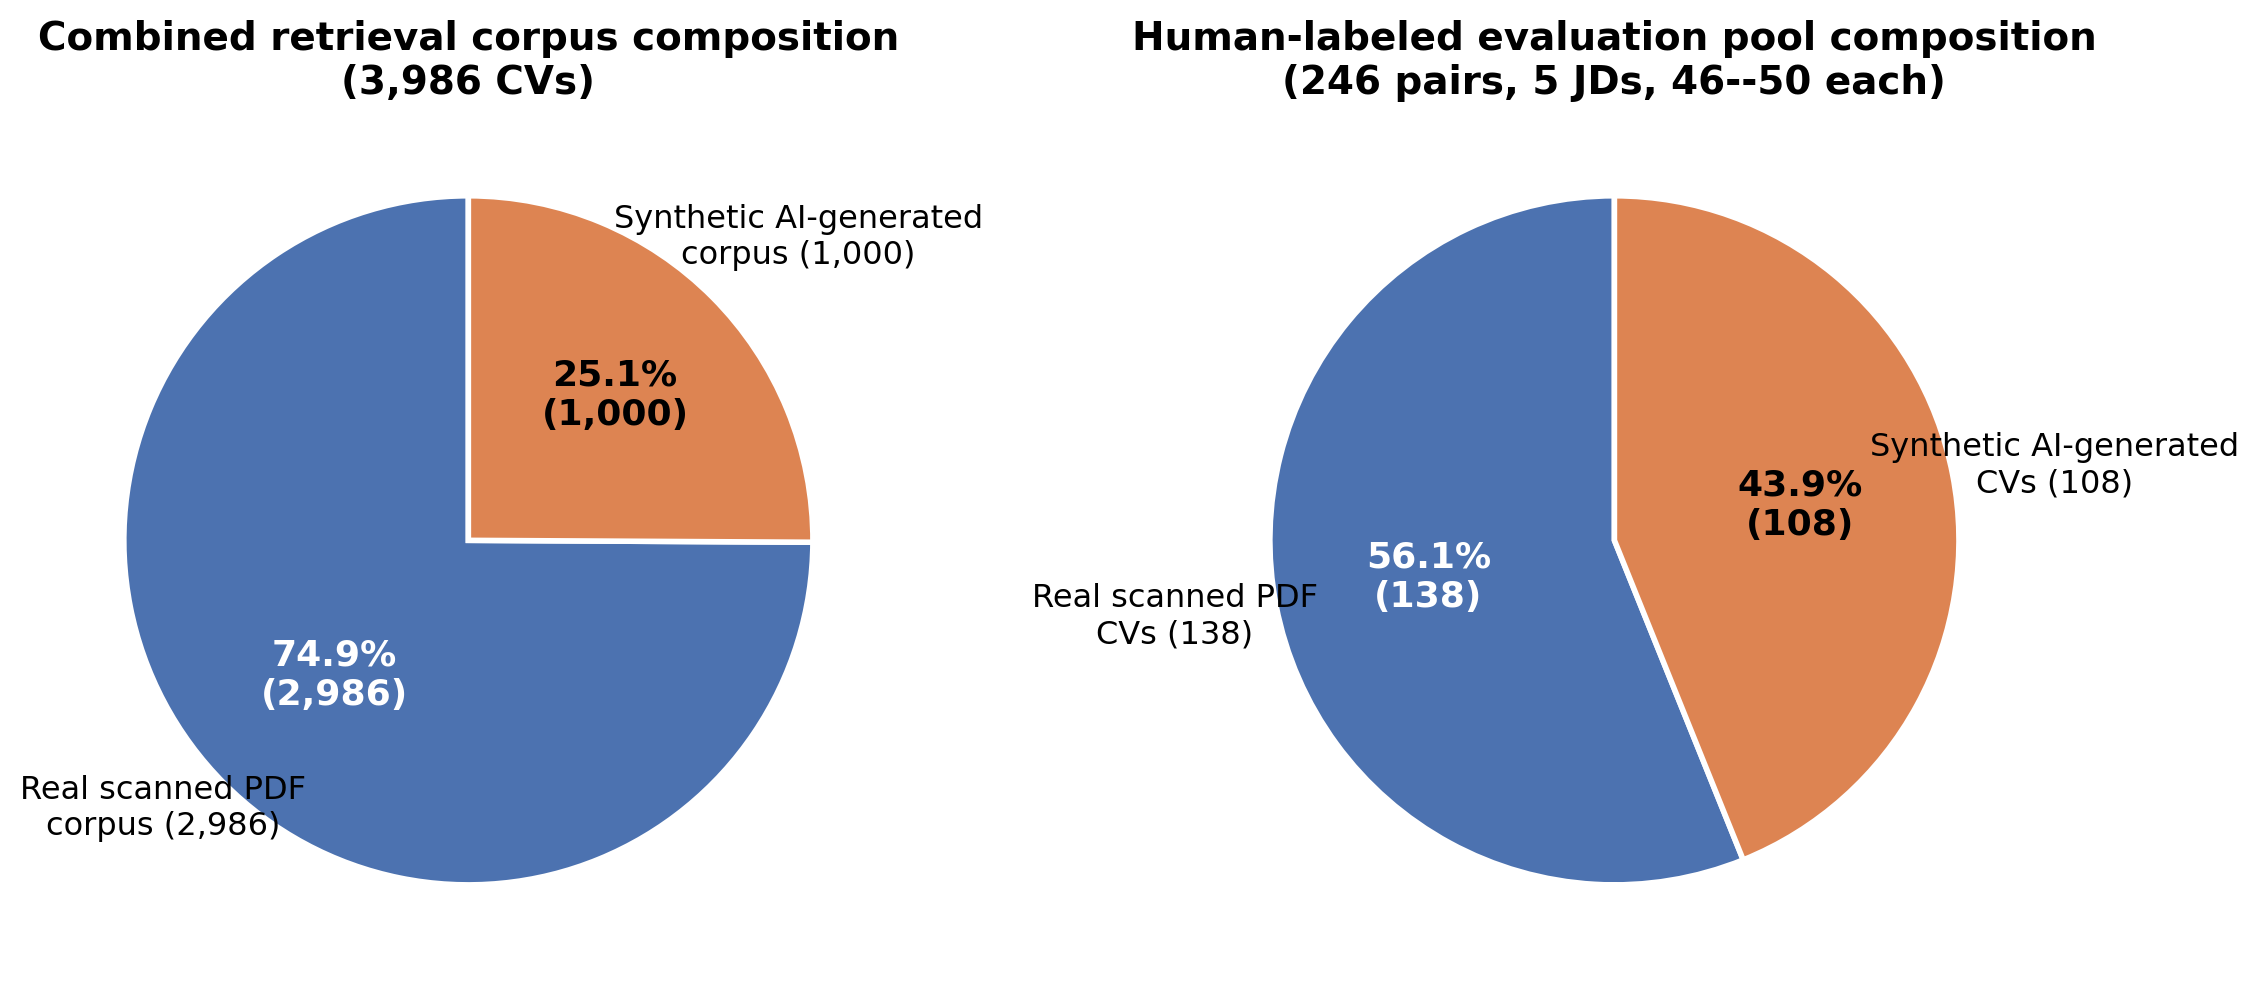
\includegraphics[width=0.98\textwidth]{figures/figure_4_2_dataset_composition.png}
\caption{Dataset composition breakdown}
\label{fig:dataset-chart}
\end{figure}

Current subset sizes (2,986 real, 1,000 synthetic, 246 labeled pairs, 3 seniority-robustness pairs, 3 keyword-stuffing triples, 3 missing-mandatory-requirement pairs, 3 role-confusion pairs) are already reported in Table~\ref{tab:dataset-composition} and are not repeated here; the remaining fields below have no value recorded yet.

\begin{table}[htbp]
\centering
\caption{Dataset documentation fields still requiring external input}
\label{tab:dataset-fields}
\begin{tabularx}{\textwidth}{>{\bfseries}p{0.32\textwidth}X}
\toprule
Field & Final value \\
\midrule
Public dataset name, URL, and license & Done -- \emph{Resume Dataset PDF} \citep{hadikpresumepdf}, \url{https://www.kaggle.com/datasets/hadikp/resume-data-pdf}, CC0: Public Domain \\
Original scanned PDF count (pre-filter) & Pending -- the system only records CVs that were successfully imported; rejected/pre-filtered files are not logged \\
OCR failure count & Pending -- failed uploads are dropped rather than logged, so a true failure count cannot be recovered retroactively; capture the upload-response JSON going forward to report this honestly \\
Duplicates and invalid records removed & Pending -- content-hash duplicate detection was added after the current 2,986 real CVs were already imported, so no historical duplicate count exists for them; new uploads from this point on are deduplicated and rejects are visible in the upload response (see Limitations for exact scope) \\
Synthetic generator and prompt version & Pending external input \\
Evaluation JDs and roles & Selected: EVAL\_JD\_01 Senior Java Developer, EVAL\_JD\_02 Junior Java Developer, EVAL\_JD\_03 Senior React Developer, EVAL\_JD\_04 Senior .NET Developer, EVAL\_JD\_05 Solution Architect (of 61 JD records in the system, including the 8 purpose-built robustness-battery JDs) \\
Development/evaluation split & Done for $\tau$-calibration purposes -- fixed-seed 50/50 per-JD split of the 246 labeled pairs into development/test halves (\cref{sec:calibration}, Table~\ref{tab:threshold-calibration}); no separate CV-corpus-level development/evaluation partition beyond this is used \\
\bottomrule
\end{tabularx}
\end{table}

\section{Relevance Labeling}
Reviewer labels use a 0--3 graded scale. Human judgments are the primary ground truth for ranking effectiveness. Synthetic manifest labels are used only to verify controlled scenarios and do not replace reviewer relevance judgments:
\begin{table}[htbp]
\centering
\caption{Manual relevance scale}
\label{tab:labels}
\begin{tabularx}{\textwidth}{cp{0.22\textwidth}X}
\toprule
Label & Meaning & Reviewer interpretation \\
\midrule
0 & Not relevant & Fails core role requirements or belongs to another role \\
1 & Weakly relevant & Some overlap but major mandatory, experience, or seniority gaps \\
2 & Relevant & Satisfies several important requirements with acceptable gaps \\
3 & Highly relevant & Strong mandatory, experience, seniority, responsibility, and evidence match \\
\bottomrule
\end{tabularx}
\end{table}

Reviewers evaluate mandatory skills, optional skills, experience relevance, minimum years, seniority, responsibility coverage, and evidence strength. The following rubric standardizes judgment without replacing reviewer expertise.

\begin{table}[htbp]
\centering
\caption{Reviewer labeling rubric}
\label{tab:label-rubric}
\begin{tabularx}{\textwidth}{p{0.28\textwidth}p{0.16\textwidth}X}
\toprule
Criterion & Guidance weight & Review guidance \\
\midrule
Mandatory skill fit & 30\% & Confirm whether core technologies or equivalent competencies are present and evidenced \\
Relevant experience & 25\% & Assess role and responsibility relevance, not only job title \\
Minimum years & 15\% & Compare explicit or date-derived experience with the JD requirement \\
Seniority alignment & 15\% & Consider ownership, design, production support, and mentoring evidence \\
Responsibility evidence & 15\% & Verify that important JD responsibilities have supporting CV sentences \\
\bottomrule
\end{tabularx}
\end{table}

The percentages guide reviewer attention; they are not used as the proposed ranking formula.

Reviewers work from anonymized candidate identifiers, the target JD, and requirement-level evidence sentences and structured fields, and are instructed not to use names, demographic attributes, photographs, or exact addresses in judgment. Because the current CV viewer displays the original, unredacted PDF (\cref{sec:security}; Chapter 5, Limitations), this is currently manual reviewer discipline rather than an enforced UI redaction; a redacted export would be needed to make it a technical control.

\Cref{fig:app-labeling} shows a candidate card's \emph{Reviewer relevance label} control with one of the four levels selected, a short note entered, and the \emph{Saved} confirmation visible on the button -- demonstrating that the labels used for Table~\ref{tab:ranking-results} are collected in-product rather than through an external spreadsheet.

\begin{figure}[htbp]
\centering
\appscreenshot{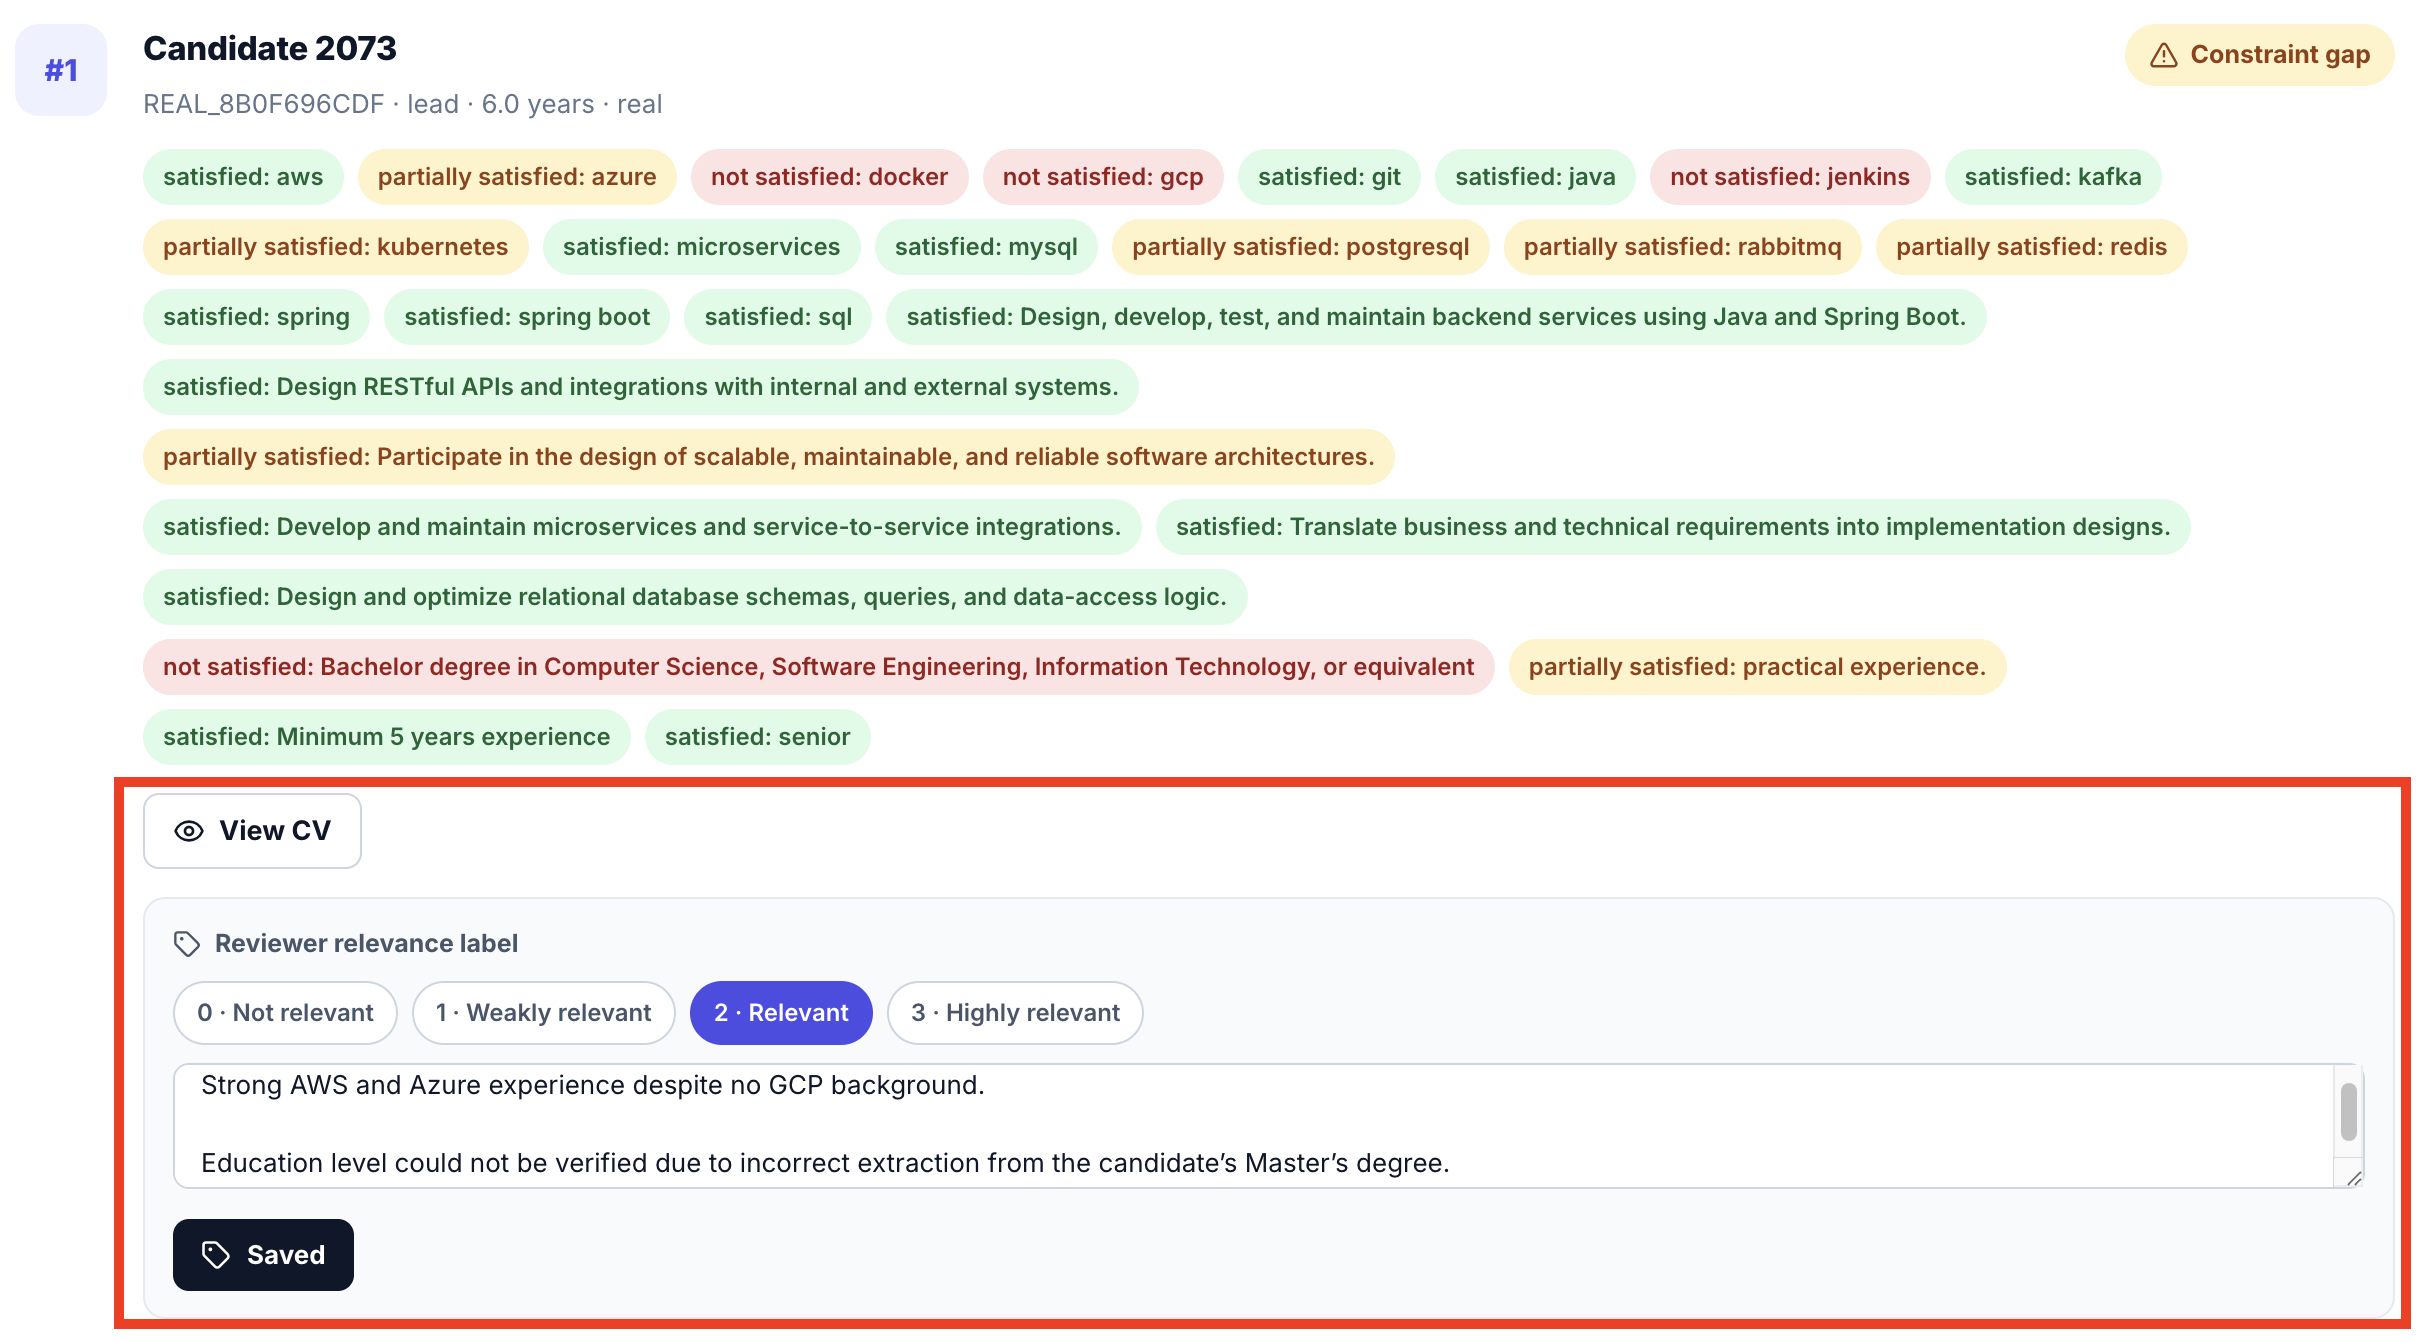
\includegraphics[width=0.92\textwidth]{figures/figure_4_3_reviewer_labeling_interface.png}}
\caption{Reviewer relevance-labeling interface}
\label{fig:app-labeling}
\end{figure}

\subsection{Reviewer Agreement and Explanation Usability}
If two reviewers are available, weighted Cohen's kappa is reported \citep{cohen1968} for the graded labels. If only one reviewer is available, the report states the reviewer profile, preserves comments, and treats single-reviewer judgment as a limitation.

To answer RQ5, a small pilot usability assessment is conducted with \texttt{Pending} recruiters, technical leads, or experienced interviewers. Participants review selected ranked candidates and rate explanation clarity, usefulness, trust, and ability to identify candidate gaps on a five-point Likert scale. If the pilot cannot be completed, RQ5 and the corresponding conclusions are explicitly limited to the design and content of the explanation output rather than demonstrated user benefit.

\begin{table}[htbp]
\centering
\caption{Explanation usability reporting template}
\label{tab:usability}
\begin{tabularx}{\textwidth}{X p{0.22\textwidth}}
\toprule
Item & Final result \\
\midrule
Number and profile of participants & Pending \\
Explanation clarity (1--5) & Pending \\
Usefulness for identifying gaps (1--5) & Pending \\
Trust in requirement-level evidence (1--5) & Pending \\
Perceived screening support (1--5) & Pending \\
Qualitative comments & Pending \\
\bottomrule
\end{tabularx}
\end{table}

\section{Experimental Models}
The model comparison is performed in three experiment groups:
\begin{enumerate}
  \item \textbf{Human-labeled effectiveness}: human-labeled pairs (a mixed real/synthetic pool, \cref{sec:labeled-pool}), reporting ranking metrics and per-JD analysis;
  \item \textbf{Controlled robustness}: seniority mismatch, unsupported claims and keyword-stuffing, missing mandatory requirements, and role confusion;
  \item \textbf{Combined-corpus performance}: indexing, latency, and response-time measurements.
\end{enumerate}

\begin{table}[htbp]
\centering
\caption{Experimental model comparison}
\label{tab:models}
\begin{tabularx}{\textwidth}{p{0.10\textwidth}p{0.30\textwidth}X}
\toprule
ID & Model & Purpose \\
\midrule
M1 & TF--IDF full text & Lexical baseline \\
M2 & SBERT full text & Semantic baseline \\
M3 & Section-level SBERT & Section-aware baseline \\
M4 & Requirement-aware matching & Tests JD decomposition and requirement coverage \\
M5 & Requirement + seniority constraints & Measures reduction of experience and seniority mismatch \\
M6 & Full proposed model & Requirement-aware, evidence-aware, constraint-based reranking \\
\bottomrule
\end{tabularx}
\end{table}

\Cref{fig:app-experiments} shows the Experiments tab after running a comparison for a JD that already has reviewer labels: the NDCG@5/NDCG@10/MAP/MRR/Recall@10/Recall@20 metrics table for all six models above, together with per-model top-ranked-candidate preview cards below it, so the figure shows both the aggregate metrics and a concrete rank-order difference between models.

\begin{figure}[htbp]
\centering
\appscreenshot{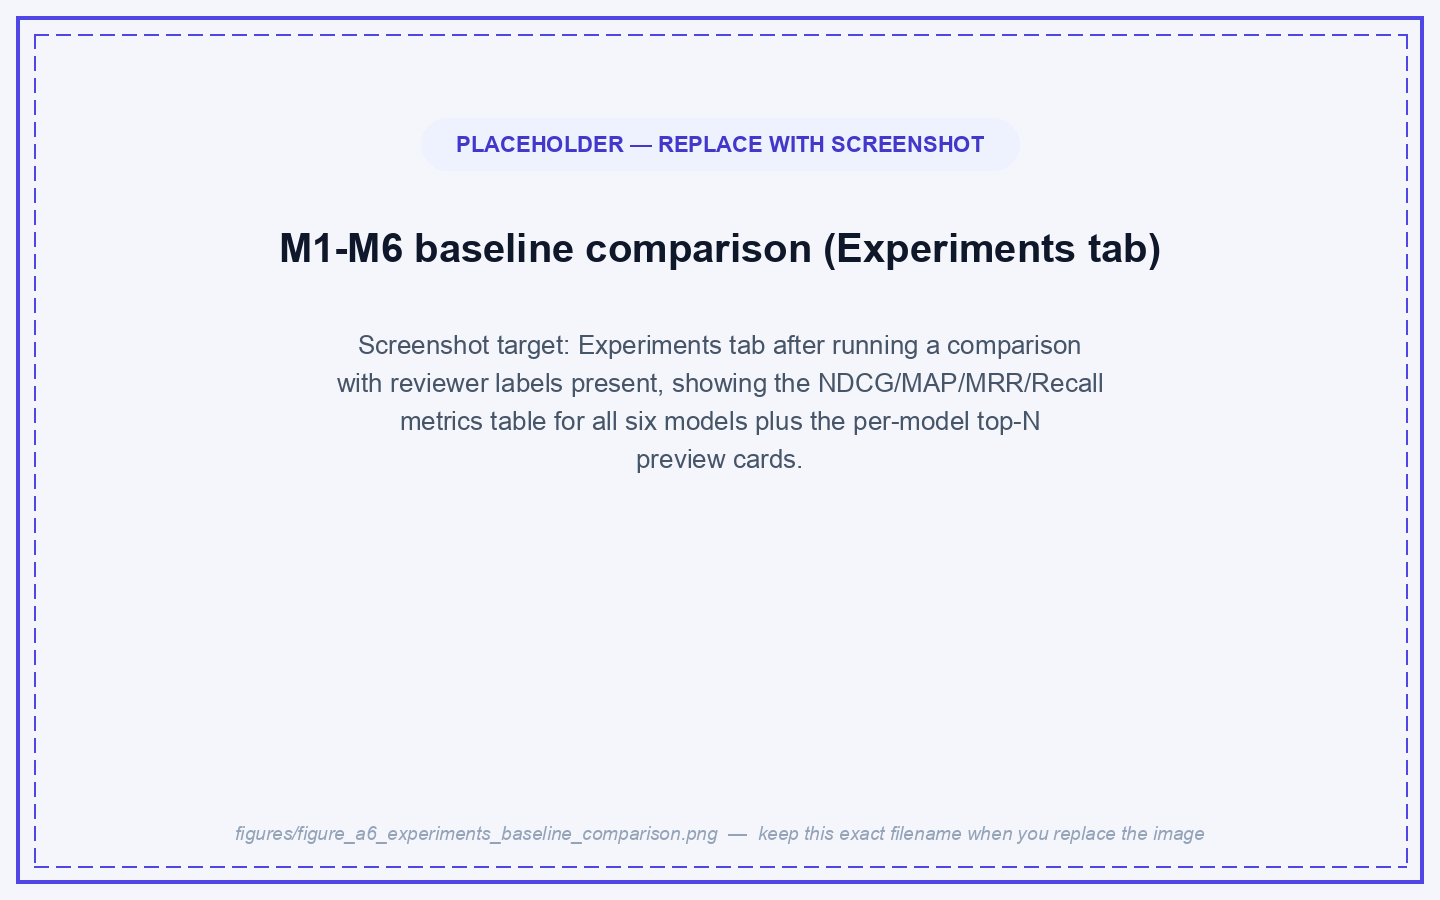
\includegraphics[width=0.92\textwidth]{figures/figure_4_4_experiments_baseline_comparison.png}}
\caption{M1--M6 baseline comparison (Experiments tab)}
\label{fig:app-experiments}
\end{figure}

\section{Ranking Metrics}
\label{sec:ranking-metrics}
The main metrics are:
\begin{itemize}
  \item \textbf{NDCG@5 and NDCG@10}: reward highly relevant candidates near the top \citep{jarvelin2002};
  \item \textbf{MAP}: evaluates precision across relevant candidates;
  \item \textbf{MRR}: measures how early the first relevant candidate appears;
  \item \textbf{Recall@10 and Recall@20}: measure shortlist coverage;
  \item \textbf{Constraint violation rate@k}: proportion of top-$k$ candidates that violate hard constraints;
  \item \textbf{Unsupported claim rate@k}: proportion of matched skills without supporting evidence.
\end{itemize}

The additional rates directly test whether the proposed mechanism solves the practical false-positive problem.

\section{Ablation Study}
The ablation study adds one mechanism at a time:
\begin{equation}
\text{SBERT} \rightarrow \text{Section matching} \rightarrow \text{Requirements} \rightarrow \text{Seniority constraints} \rightarrow \text{Evidence verification}.
\end{equation}

This shows whether each component contributes to ranking improvement, rather than relying on an opaque final model, and is run on the human-labeled pool (controlled synthetic cases are reported separately). The chain corresponds directly to models M2--M6 in Table~\ref{tab:ranking-results} (M1 TF--IDF is a separate lexical baseline, not part of the chain), so the per-step effect is already visible in that table rather than needing a separate ablation table: each added mechanism (Section matching, Requirements, Seniority, Evidence verification) leaves ranking quality flat or lower than the step before it, which is the basis for the RQ1/RQ2 finding in \cref{sec:discussion}.

\subsection{Threshold Sensitivity}
The lower and higher evidence thresholds $\tau_l$ and $\tau_h$ were left at their prototype defaults ($0.35$/$0.55$) for every other result in this thesis rather than calibrated on a development subset; \cref{sec:discussion} identifies this as one of two likely causes of the requirement-decomposition family's ranking-effectiveness result. Since only the full model (M6) uses these thresholds (M4/M5 assess declared skills only, without semantic evidence verification), the sensitivity analysis re-runs M6 alone, at four $(\tau_l,\tau_h)$ pairs, against the same 246-pair labeled pool used for Table~\ref{tab:ranking-results}.

\begin{table}[htbp]
\centering
\caption{Evidence-threshold sensitivity (M6, full proposed model)}
\label{tab:threshold-sensitivity}
\begin{tabular}{lccc}
\toprule
$(\tau_l,\tau_h)$ & Macro NDCG@10 & Macro MAP & Hard-pass rate \\
\midrule
$(0.20, 0.40)$ & 0.3072 & 0.4385 & 0\% \\
$(0.35, 0.55)$ -- prototype default & 0.2953 & 0.4216 & 0\% \\
$(0.45, 0.65)$ & 0.4914 & 0.5807 & 0\% \\
$(0.55, 0.75)$ & 0.5311 & 0.5834 & 0\% \\
\bottomrule
\end{tabular}
\end{table}

This run used the corpus as it stood at the time (3,991 CVs, grown from 3,986 by the purpose-built robustness-test records added earlier in the same session, \cref{sec:robustness-sets}); this is why the $(0.35,0.55)$ row above (0.2953) does not exactly reproduce the 0.3422 macro NDCG@10 for M6 in Table~\ref{tab:ranking-results} -- a few extra unlabeled candidates can shift which labeled candidates fall inside a top-10 window for a 46--50-pair-per-JD set. All four rows share one fixed snapshot, so the trend across thresholds is the valid takeaway even though the absolute baseline differs slightly from the headline table.

Two findings follow. First, the trend is not monotonic and the shipped default is the weakest of the four settings: NDCG@10 is 0.3072 at the lenient $(0.20,0.40)$ pair, dips to 0.2953 at the default $(0.35,0.55)$, then rises to 0.4914 and 0.5311 as thresholds tighten. The strictest pair, $(0.55,0.75)$, is best -- roughly $1.8\times$ the default -- the opposite of \cref{sec:discussion}'s initial hypothesis (that the default was too strict); the data instead says the default is slightly too \emph{lenient}, and tightening is the more promising calibration direction. Even the best setting remains far below the SBERT-full-text baseline (NDCG@10 0.96), so recalibrating $\tau$ alone would not close the gap. Second, the hard-pass rate is 0\% at every threshold tested, confirming $\tau_l$/$\tau_h$ are not why $H_{\mathrm{pass}}$ fails to discriminate: the undifferentiated-hard-constraint mechanism (\cref{sec:discussion}) is the dominant cause, and no evidence-threshold retuning changes it, since $H_{\mathrm{pass}}$ requires \emph{every} hard requirement individually satisfied regardless of how permissive "satisfied" is.

\subsubsection{Calibration on a Held-out Development Split}
\label{sec:calibration}
The sensitivity probe above answers whether $\tau$ matters, but picking the best-looking pair directly against the same 246 labeled pairs used for the headline result would be test-set leakage. Proper calibration instead requires tuning on a development subset and confirming the choice on a held-out test subset it never saw. Each of the 5 JDs' labeled pairs was split 50/50 into development and test halves (fixed seed, 23--25 pairs per half per JD), and M6 was re-run at 6 evenly spaced $(\tau_l,\tau_h)$ pairs (fixed $0.20$ gap, $(0.20,0.40)$ to $(0.70,0.90)$), scored against the development half only.

\begin{table}[htbp]
\centering
\caption{Threshold calibration on a held-out development/test split (M6)}
\label{tab:threshold-calibration}
\begin{tabular}{lccc}
\toprule
$(\tau_l,\tau_h)$ & Dev macro NDCG@10 & Test macro NDCG@10 & Full-pool macro NDCG@10 \\
\midrule
$(0.20, 0.40)$ & 0.4580 & 0.4127 & 0.3031 \\
$(0.30, 0.50)$ & 0.3438 & 0.3055 & 0.2463 \\
$(0.40, 0.60)$ & 0.4698 & 0.4534 & 0.3435 \\
\textbf{$(0.50, 0.70)$} & \textbf{0.5828} & \textbf{0.5687} & \textbf{0.4494} \\
$(0.60, 0.80)$ & 0.5657 & 0.6036 & 0.4762 \\
$(0.70, 0.90)$ & 0.5228 & 0.6212 & 0.4869 \\
\bottomrule
\end{tabular}
\end{table}

The pair $(\tau_l,\tau_h)=(0.50,0.70)$ has the highest development-split NDCG@10 (0.5828) and was selected on that basis alone, without looking at the test half; its held-out test-split score (0.5687) is close to its development value, so the selection generalizes rather than overfits. Against the full 246-pair pool, this calibrated pair reaches macro NDCG@10 of 0.4494 -- a genuine, held-out-validated improvement of roughly $52\%$ over the shipped default's 0.2953 (same corpus snapshot), though still far below the SBERT-full-text baseline's 0.9632. One caveat: $(0.70,0.90)$'s test-split score (0.6212) exceeds $(0.50,0.70)$'s (0.5687), so the exact optimum is somewhat sensitive to which pairs fell into the development half -- expected sampling noise at only 23--25 pairs per JD per half, not a stable ranking of the two settings. The robust conclusion is the broader trend: every setting at $\tau_l \geq 0.40$ outperforms the two most lenient settings on both halves, so a properly calibrated M6 should use a stricter evidence threshold than the current default, consistent with \cref{sec:discussion}.

This calibration is threshold-only, and only M6 has thresholds to tune ($\tau_l$, $\tau_h$); M1--M5 were never re-scored on this same development/test split, since M1--M3 are parameter-free and M4/M5 use declared-only assessment with no evidence threshold. Consequently, the 0.4494-vs-0.9632 comparison above is not a fully like-for-like held-out comparison: the 0.4494 figure benefits from a threshold chosen using half of the very 246-pair pool it is then scored against, while the 0.9632 SBERT figure required no such fitting on any part of that pool. A strictly controlled comparison would score all six models on the identical held-out test half alone; this thesis's schedule did not extend to that additional run, and the gap is reported with this caveat attached rather than presented as a clean apples-to-apples result.

\section{Seniority Mismatch Robustness Test}
The test set includes JDs with explicit minimum years and seniority levels. Candidate CVs are grouped as Intern/Fresher, Junior, Middle, Senior, Lead, and Architect. The main measurement is whether underqualified candidates appear in the top-$k$ list.

Example test:
\begin{quote}
JD: Senior Java Developer, minimum 5 years, system design and mentoring.\\
CV A: Fresher with Java, Spring Boot, SQL, Docker.\\
CV B: Senior candidate with 6 years, microservices, production troubleshooting, and mentoring.
\end{quote}

Similarity-only methods may rank CV A highly because of skill overlap. The proposed mechanism should rank CV B above CV A because the hard constraints and evidence are stronger.

\section{Keyword-stuffing Robustness Test}
A controlled adversarial test is created by adding unrelated or unsupported skills to a CV Skills section without adding project or experience evidence. The rank change is measured before and after manipulation.

\begin{table}[htbp]
\centering
\caption{Keyword-stuffing test design}
\label{tab:stuffing}
\begin{tabularx}{\textwidth}{p{0.28\textwidth}XX}
\toprule
Version & Modification & Expected behavior \\
\midrule
Original CV & Skills and evidence remain consistent & Stable ranking \\
Stuffed CV & Add AWS, Kubernetes, Kafka, Spark, React, TensorFlow to Skills only & Similarity baseline may increase; evidence-aware rank should not materially increase \\
Supported CV & Add the same skills with project evidence & Ranking may increase if requirements are relevant \\
\bottomrule
\end{tabularx}
\end{table}

\section{PDF and OCR Evaluation}
The ingestion evaluation reports:
\begin{itemize}
  \item direct extraction success rate;
  \item OCR fallback success rate;
  \item extracted character count;
  \item section detection completeness;
  \item processing time per CV;
  \item failure reasons.
\end{itemize}

OCR reliability is evaluated only on the real scanned Kaggle subset. Synthetic text-layer PDFs are excluded from the OCR success rate and are used instead for controlled ranking and scalability tests. OCR is not the primary research contribution, but extraction quality is documented because it directly affects downstream evidence retrieval and ranking.

\section{Result Tables}
The table structures below were fixed before experimentation to reduce selective reporting. All quantitative cells are populated from the reproducible runs described in this chapter; any cell not yet backed by a completed run is marked \texttt{Pending} explicitly rather than left ambiguous.

\begin{table}[htbp]
\centering
\caption{Ranking effectiveness on the human-labeled pool (real + synthetic)}
\label{tab:ranking-results}
\begin{adjustbox}{max width=\textwidth}
\begin{tabular}{lcccccc}
\toprule
Model & NDCG@5 & NDCG@10 & MAP & MRR & Recall@10 & Recall@20 \\
\midrule
TF--IDF & 0.8806 & 0.8956 & 0.9009 & 1.0000 & 0.4980 & 0.7351 \\
SBERT full text & \textbf{0.9489} & \textbf{0.9632} & \textbf{0.9759} & 1.0000 & \textbf{0.5460} & \textbf{0.7968} \\
Section-level SBERT & 0.8395 & 0.8359 & 0.9154 & 1.0000 & 0.4973 & 0.7714 \\
Requirement-aware & 0.3769 & 0.4369 & 0.5307 & 0.7250 & 0.2456 & 0.4153 \\
Requirement + seniority & 0.3639 & 0.4235 & 0.5186 & 0.7250 & 0.2331 & 0.4066 \\
Full proposed model & 0.2938 & 0.3422 & 0.4553 & 0.8250 & 0.1614 & 0.3144 \\
\bottomrule
\end{tabular}
\end{adjustbox}
\end{table}

Values are macro-averaged over the five evaluation JDs (EVAL\_JD\_01--05), each contributing 46--50 reviewer-labeled candidates (246 pairs, single reviewer), so no JD dominates the mean. All six models are ranked against the full indexed corpus (3,986 CVs) and scored against the identical 246-pair labeled set. \textbf{The three similarity-only baselines (M1--M3) outperform the requirement-decomposition family (M4--M6) on every metric except MRR, and the full proposed model (M6) is the weakest of the six on NDCG@5, NDCG@10, MAP, and Recall@10/20.} This holds per-JD, not just on average (Table~\ref{tab:per-jd-ndcg10}), and survives removal of two JD-parsing artifacts found during this run (a stray control character on auto-extracted bullets, a disclaimer sentence mis-parsed as a soft requirement), so it is not an artifact of those bugs. \Cref{sec:discussion} discusses the likely mechanism.

\begin{table}[htbp]
\centering
\caption{Constraint-violation and unsupported-claim rates at $k{=}10$}
\label{tab:violation-rates}
\begin{tabular}{lccc}
\toprule
JD & M5 violation rate@10 & M6 violation rate@10 & M6 unsupported-claim rate@10 \\
\midrule
EVAL\_JD\_01 & 100\% & 100\% & 2.78\% \\
EVAL\_JD\_02 & 100\% & 100\% & 1.53\% \\
EVAL\_JD\_03 & 100\% & 100\% & 0.00\% \\
EVAL\_JD\_04 & 100\% & 100\% & 1.14\% \\
EVAL\_JD\_05 & 100\% & 100\% & 0.53\% \\
\textbf{Macro-avg} & \textbf{100\%} & \textbf{100\%} & \textbf{1.20\%} \\
\bottomrule
\end{tabular}
\end{table}

The two rate-style metrics from \cref{sec:ranking-metrics} are computed directly on each model's actual top-10 candidates from the full 3,986-CV corpus, not only on the 46--50 labeled candidates per JD used for Table~\ref{tab:ranking-results}. \textbf{Constraint violation rate@10 is 100\% for both M5 and M6 on all five JDs}: every top-10 slot either constraint-gated model produces contains a candidate who fails at least one hard requirement. This sharply confirms the 0\% hard-pass rate already seen at every $\tau$ setting (Table~\ref{tab:threshold-sensitivity}): the hard-pass gate in \cref{eq:ranking-key} is not just weak but entirely non-operative at the top of the ranked list here, since no fully-hard-passing candidate exists in the corpus under the auto-parsed requirement lists (\cref{sec:discussion}). In sharp contrast, M6's unsupported-claim rate@10 is low -- 1.20\% macro-averaged (0.00\%--2.78\% across JDs) -- meaning the skills credited to M6's own top-10 candidates are overwhelmingly genuinely evidence-supported, not merely declared. This favorable, standalone result for evidence verification reinforces \cref{sec:discussion}'s diagnosis: the undifferentiated hard-constraint mechanism, not the evidence threshold, is the dominant cause of M6's low ranking-effectiveness metrics.

\begin{table}[htbp]
\centering
\caption{Per-JD NDCG@10 breakdown}
\label{tab:per-jd-ndcg10}
\begin{adjustbox}{max width=\textwidth}
\begin{tabular}{lcccccc}
\toprule
Model & EVAL\_JD\_01 & EVAL\_JD\_02 & EVAL\_JD\_03 & EVAL\_JD\_04 & EVAL\_JD\_05 & Macro-avg \\
\midrule
TF--IDF & 0.8175 & 0.7049 & 1.0000 & 0.9556 & 1.0000 & 0.8956 \\
SBERT full text & 0.9155 & 0.9005 & 1.0000 & 1.0000 & 1.0000 & 0.9632 \\
Section-level SBERT & 0.8716 & 0.5584 & 0.7926 & 0.9571 & 1.0000 & 0.8359 \\
Requirement-aware & 0.6315 & 0.3543 & 0.6685 & 0.2748 & 0.2553 & 0.4369 \\
Requirement + seniority & 0.5937 & 0.3543 & 0.6685 & 0.2748 & 0.2264 & 0.4235 \\
Full proposed model & 0.3276 & 0.3386 & 0.5666 & 0.2147 & 0.2633 & 0.3422 \\
\bottomrule
\end{tabular}
\end{adjustbox}
\end{table}

On every one of the five JDs, all three similarity-only baselines (M1--M3) score strictly higher NDCG@10 than all three requirement-decomposition models (M4--M6), so the macro-average finding is not an artifact of one JD dominating the mean. Within M4--M6, M4 and M5 are the two highest on four of five JDs; the exception is EVAL\_JD\_05, where M6 (0.2633) slightly beats both M4 (0.2553) and M5 (0.2264) -- reported here rather than smoothed away, consistent with this thesis's commitment not to round results toward the expected direction.

\begin{table}[htbp]
\centering
\caption{Bootstrap 95\% confidence intervals (resampling the 5 JDs, $B{=}10{,}000$)}
\label{tab:bootstrap-ci}
\begin{tabular}{lcc}
\toprule
Model & NDCG@10 (95\% CI) & MAP (95\% CI) \\
\midrule
TF--IDF & 0.8956 [0.7864, 0.9911] & 0.9009 [0.8590, 0.9473] \\
SBERT full text & 0.9632 [0.9234, 1.0000] & 0.9759 [0.9502, 0.9964] \\
Section-level SBERT & 0.8359 [0.6850, 0.9572] & 0.9154 [0.8740, 0.9612] \\
Requirement-aware & 0.4369 [0.2829, 0.5909] & 0.5307 [0.3487, 0.7302] \\
Requirement + seniority & 0.4235 [0.2713, 0.5757] & 0.5186 [0.3223, 0.7126] \\
Full proposed model & 0.3422 [0.2536, 0.4603] & 0.4553 [0.2862, 0.6336] \\
\bottomrule
\end{tabular}
\end{table}

\begin{table}[htbp]
\centering
\caption{Paired comparison with the full proposed model (M6), $n{=}5$ JDs}
\label{tab:paired-significance}
\begin{tabular}{lcccc}
\toprule
Baseline & NDCG@10 mean diff [95\% CI] & Wilcoxon $p$ & MAP mean diff [95\% CI] & Wilcoxon $p$ \\
\midrule
TF--IDF & $+0.5534$ [$+0.4179$, $+0.6890$] & 0.0625 & $+0.4456$ [$+0.2910$, $+0.6056$] & 0.0625 \\
SBERT full text & $+0.6210$ [$+0.5157$, $+0.7309$] & 0.0625 & $+0.5206$ [$+0.3527$, $+0.6933$] & 0.0625 \\
Section-level SBERT & $+0.4938$ [$+0.2871$, $+0.7004$] & 0.0625 & $+0.4601$ [$+0.3057$, $+0.6253$] & 0.0625 \\
Requirement-aware & $+0.0947$ [$+0.0151$, $+0.2059$] & 0.125 & $+0.0754$ [$+0.0280$, $+0.1227$] & 0.0625 \\
Requirement + seniority & $+0.0814$ [$+0.0019$, $+0.1832$] & 0.1875 & $+0.0633$ [$+0.0075$, $+0.1191$] & 0.1875 \\
\bottomrule
\end{tabular}
\end{table}

The bootstrap CIs are computed by resampling the 5 JDs with replacement (the standard unit for query-level IR metrics) and taking the 2.5th/97.5th percentile of the resampled macro-average. Individual-method CIs (Table~\ref{tab:bootstrap-ci}) are wide, as expected with only 5 queries, but the \emph{paired} bootstrap CI on the difference against M6 (Table~\ref{tab:paired-significance}) excludes zero for all three similarity-only baselines on both metrics, and excludes zero (barely, on MAP) or comes close to it (NDCG@10) for M4/M5 -- consistent with \cref{sec:discussion}'s reading that the M4--M6 gap is smaller and noisier than the baseline-vs-M6 gap. The Wilcoxon signed-rank test, however, cannot reach $p<0.05$ for \emph{any} comparison: with $n=5$ paired observations, the smallest possible exact two-sided $p$-value is $1/16=0.0625$, achieved here for every baseline-vs-M6 comparison (all 5 JDs agree in sign) but never able to cross $0.05$ regardless of effect size. This is reported as a limitation, not omitted: the paired bootstrap CI is more informative here since it uses actual effect magnitude rather than only rank, and it agrees with \cref{sec:discussion}'s qualitative finding -- but neither substitutes for a larger-JD-count study (\cref{sec:future-work}).

\Cref{fig:ranking-effectiveness-chart} plots all six metrics from Table~\ref{tab:ranking-results} by model, with the best-performing model on each metric outlined in black; the three similarity-only baselines (M1--M3) visibly dominate the requirement-decomposition family (M4--M6) on every metric except MRR.

\begin{figure}[htbp]
\centering
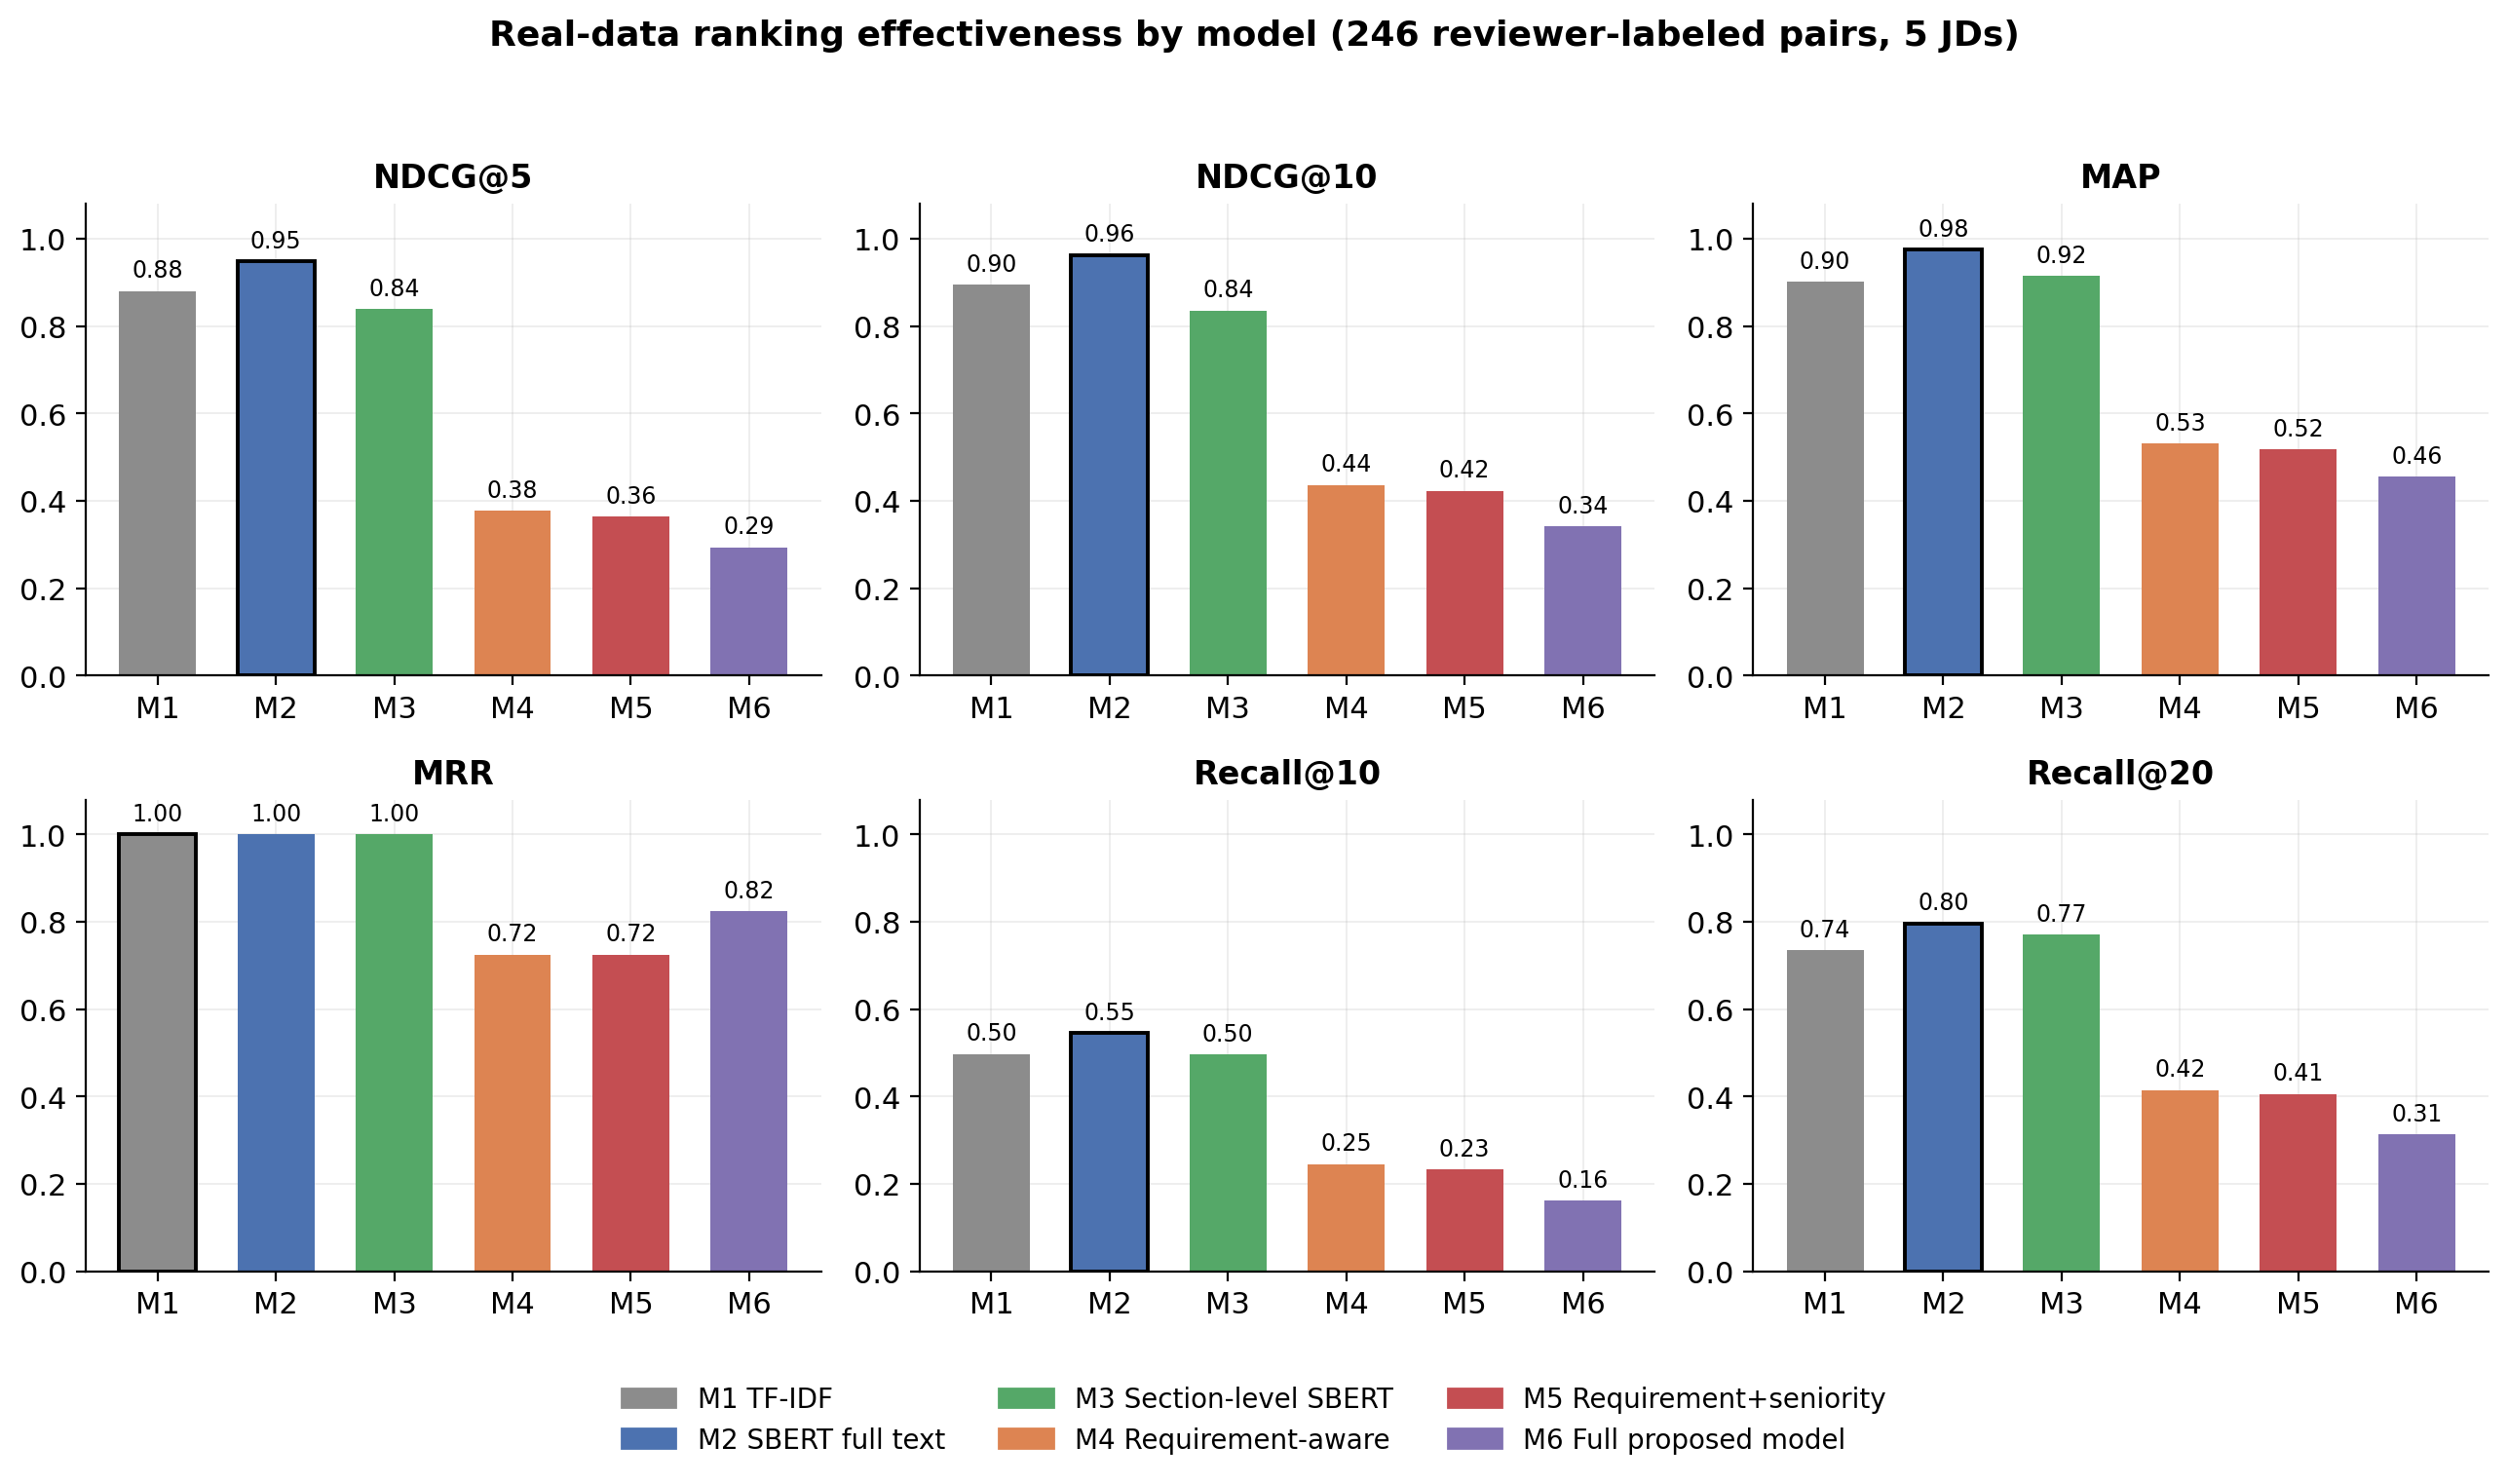
\includegraphics[width=0.98\textwidth]{figures/figure_4_5_ranking_effectiveness_comparison.png}
\caption{Ranking effectiveness by model (human-labeled pool)}
\label{fig:ranking-effectiveness-chart}
\end{figure}

\begin{table}[htbp]
\centering
\caption{Controlled robustness results}
\label{tab:robustness-results}
\begin{adjustbox}{max width=\textwidth}
\begin{tabular}{lccc}
\toprule
Model & Seniority mismatch (Senior rank / Fresher rank) & Rank $\Delta$ after stuffing, no evidence & Rank $\Delta$ after stuffing, with evidence \\
\midrule
TF--IDF & 1 / 822 (no hard-gate) & $-4$ (18$\to$22) & $-69$ (18$\to$87) \\
SBERT full text & 3 / 162 (no hard-gate) & $-3$ (52$\to$55) & $-739$ (52$\to$791) \\
Section-level SBERT & 65 / 192 (no hard-gate) & $-23$ (33$\to$56) & $-213$ (33$\to$246) \\
Requirement-aware & 1 / 290 (no hard-gate) & $+389$ (563$\to$174) & $+376$ (563$\to$187) \\
Requirement + seniority & 1 / 1355 (gate: pass / fail) & $+403$ (591$\to$188) & $+402$ (591$\to$189) \\
Full proposed model & 45 / 2617 (gate: fail / fail) & $+204$ (619$\to$415) & $+457$ (619$\to$162) \\
\bottomrule
\end{tabular}
\end{adjustbox}
\end{table}

All five controlled-set categories from \cref{sec:robustness-sets} were built and run: seniority mismatch (Senior/Fresher pair against a purpose-built JD requiring 5+ years, senior level, Java/Spring Boot/SQL hard and Docker soft), keyword stuffing with a supported-evidence control (Original/Stuffed/Supported triple against EVAL\_JD\_01, the 25-requirement Senior Java Developer JD from Table~\ref{tab:ranking-results}), missing mandatory requirement (pair against a purpose-built Python backend JD, Table~\ref{tab:missing-mandatory-case}), and role confusion (genuine-developer/confused-PM pair against a purpose-built Java backend JD, Table~\ref{tab:role-confusion-case}). This table reports the first two; the latter two appear as separate case-study tables below, since their natural unit is a rank pair rather than a rank-change column. All five tables share one fixed snapshot -- the full 4,013-CV corpus (\cref{sec:battery}) -- so rank denominators are directly comparable throughout (the one exception is \cref{sec:calibration}'s threshold-sensitivity analysis, which re-runs the full 246-pair evaluation and was left at its own 3,991-CV snapshot). Rank $\Delta$ is Original rank minus modified-CV rank, so positive means the modification moved the CV toward rank 1.

Because each category is a single constructed instance ($n=1$ per model), the pre-registered ``@10 rate'' columns could not be computed as specified; the table instead reports the measured outcome for the one built instance, and this adaptation is stated here explicitly rather than silently reinterpreted. For the same reason these numbers are not stable rates -- they characterize mechanism behavior on one case each, consistent with how \cref{sec:discussion} treats synthetic controlled cases generally.

For seniority mismatch, ``gate'' refers to $H_{\mathrm{pass}}$ (\cref{eq:ranking-key}): M5 gates correctly (passes Senior, fails Fresher), but M6 fails both, because its evidence-aware assessment marks the Senior CV's declared SQL skill \texttt{unsupported} -- the experience text describes Java/Spring Boot work but never restates SQL usage in prose, even though SQL is listed under Skills. This is a genuine false negative, not a labeling error: it shows M6's per-requirement evidence rule can penalize a plausible senior candidate whose resume doesn't restate every declared skill in a work-experience sentence. M1--M4 have no hard-constraint mechanism, so no gate outcome applies; M4 still separates Senior from Fresher sharply (1 vs 290) from declared-requirement coverage alone.

For stuffing, all six assessments were also checked against EVAL\_JD\_01's 23 hard requirements directly: the Original CV already fails 16/23 outright (missing azure, gcp, jenkins, mysql, postgresql, rabbitmq, redis, and others), so $H_{\mathrm{pass}}$ is \texttt{False} for all three versions regardless of stuffing -- consistent with the undifferentiated-hard-constraint mechanism (\cref{sec:discussion}), confirming the rank movement above comes entirely from post-gate coverage/evidence, not from crossing the hard gate. Adding the six stuffed skills (aws, kubernetes, kafka among them) moves their status from \texttt{not\_satisfied} to \texttt{unsupported} but leaves the unsatisfied count at 16/23; adding genuine evidence sentences (Supported CV) resolves those three to \texttt{satisfied}, reducing it to 13/23 -- the clearest evidence here that evidence verification works as designed: mere declaration is not credited, matching evidence text is. TF--IDF and the two SBERT baselines (M1: Original 18, Stuffed 22, Supported 87) all rank Stuffed and, more so, Supported \emph{worse} than Original, because appending extra vocabulary to a whole-document vector dilutes similarity to a JD written in comparatively few core terms, regardless of evidence. Requirement-aware (M4: Original 563, Stuffed 174, Supported 187) moves almost identically for Stuffed and Supported ($+389$ vs $+376$), confirming it cannot distinguish unsupported from evidenced skills, since it has no evidence-verification step. M6 is the only method where Supported improves rank clearly more than Stuffed ($+457$ vs $+204$, a 253-rank gap): evidence verification reduces but -- since \texttt{unsupported} still outscores \texttt{not\_satisfied} in the ordinal status scale (\cref{tab:assessment-rules}) -- does not eliminate the ranking benefit of keyword stuffing.

\Cref{fig:robustness-chart} visualizes Table~\ref{tab:robustness-results} by model (log scale): the left panel shows Senior vs.\ Fresher CV rank for the seniority-mismatch test, where only M5 gates correctly, and the right panel shows rank by CV version (Original/Stuffed/Supported) for the keyword-stuffing test, where M4--M6 all improve from added declared skills but only M6 improves more from genuine evidence (Supported) than from unevidenced stuffing.

\begin{figure}[htbp]
\centering
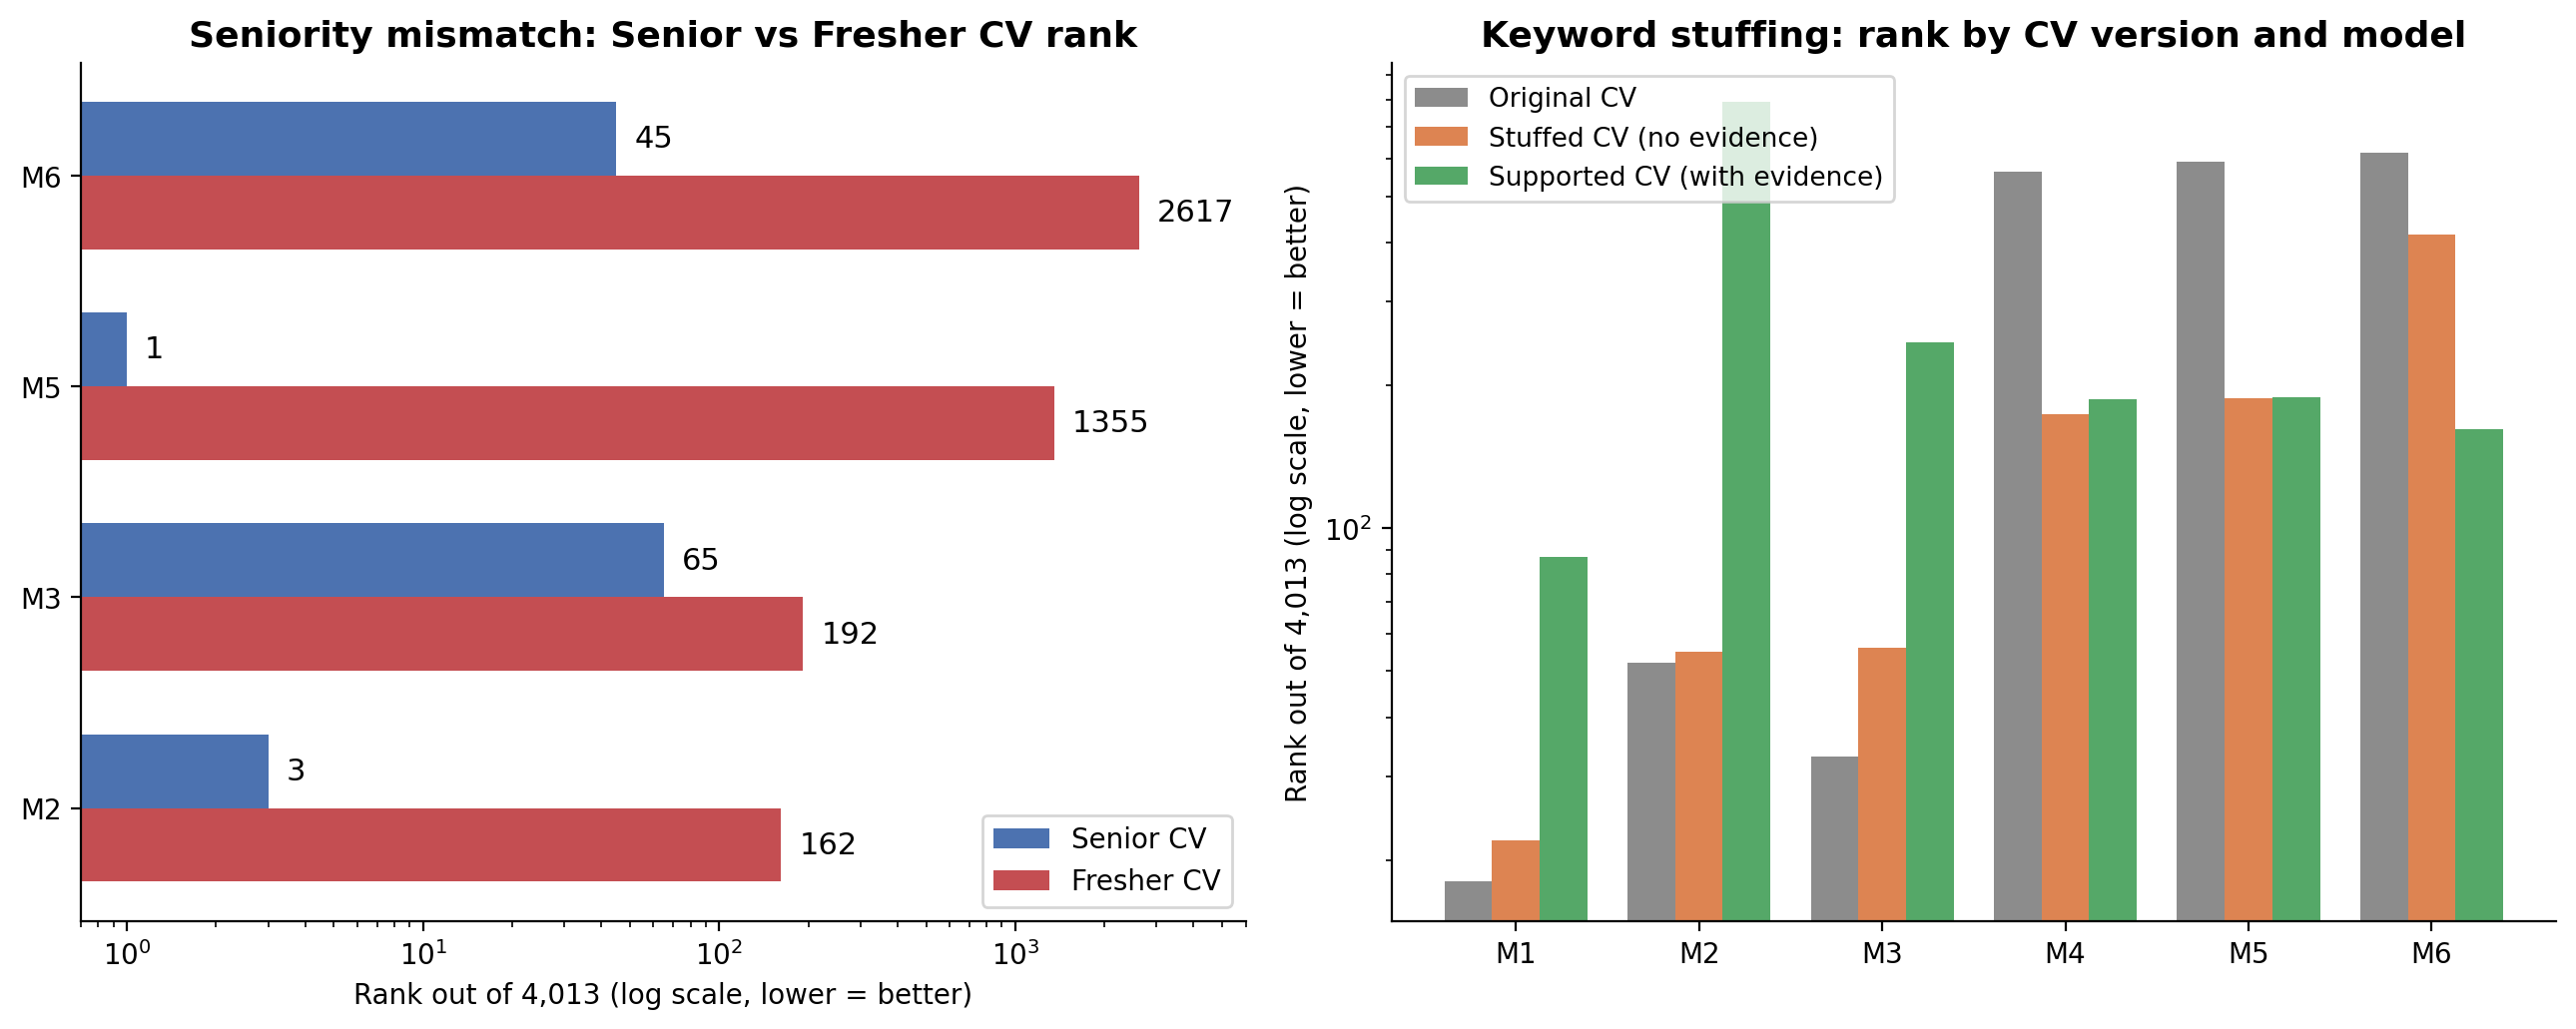
\includegraphics[width=0.98\textwidth]{figures/figure_4_6_robustness_rank_changes.png}
\caption{Controlled robustness results by model}
\label{fig:robustness-chart}
\end{figure}

\begin{table}[htbp]
\centering
\caption{Real scanned PDF OCR and parsing results}
\label{tab:ocr-results}
\begin{tabularx}{\textwidth}{X p{0.25\textwidth}}
\toprule
Metric & Final result \\
\midrule
OCR success rate & 100\% of \emph{indexed} records (2,986/2,986 currently indexed as \texttt{real} show \texttt{pdf\_\allowbreak ocr\_\allowbreak extracted}); this is tautological by construction, since a file that fails OCR is never indexed and so never enters this denominator -- it is not a claim that 100\% of attempted uploads succeed. Raw pre-filter total and true failure rate remain \texttt{Pending}, Table~\ref{tab:dataset-composition} \\
OCR failure rate & \texttt{Pending} -- failed uploads are not logged by the current pipeline, so this cannot be recovered retroactively (see Limitations) \\
Average OCR time per page & 8.08\,s (Tesseract 5.5.2 + Poppler 26.07.0, single CPU core); full benchmark detail in Table~\ref{tab:performance-results} \\
Skills-section detection rate & 69.3\% (2,070 / 2,986 real CVs) \\
Experience-section detection rate & 56.4\% (1,685 / 2,986 real CVs) \\
Experience-year correctness on inspected sample & Pending -- requires manual inspection of a drawn sample against the source PDF; the \texttt{years\_\allowbreak detected} flag can prioritize the sample toward CVs where no year phrase was found at all, versus CVs with an explicit but possibly wrong value \\
Seniority correctness on inspected sample & Pending -- requires manual inspection of a drawn sample against the source PDF \\
\bottomrule
\end{tabularx}
\end{table}

\Cref{fig:ocr-chart} plots OCR success rate against Skills/Experience-section detection coverage across the 2,986-CV real corpus (Table~\ref{tab:ocr-results}); the gap between OCR success (100\%) and section detection (69.3\%/56.4\%) reflects real scanned resumes whose text was recovered but whose layout does not use a recognizable section heading (see Limitations, Chapter 5).

\begin{figure}[htbp]
\centering
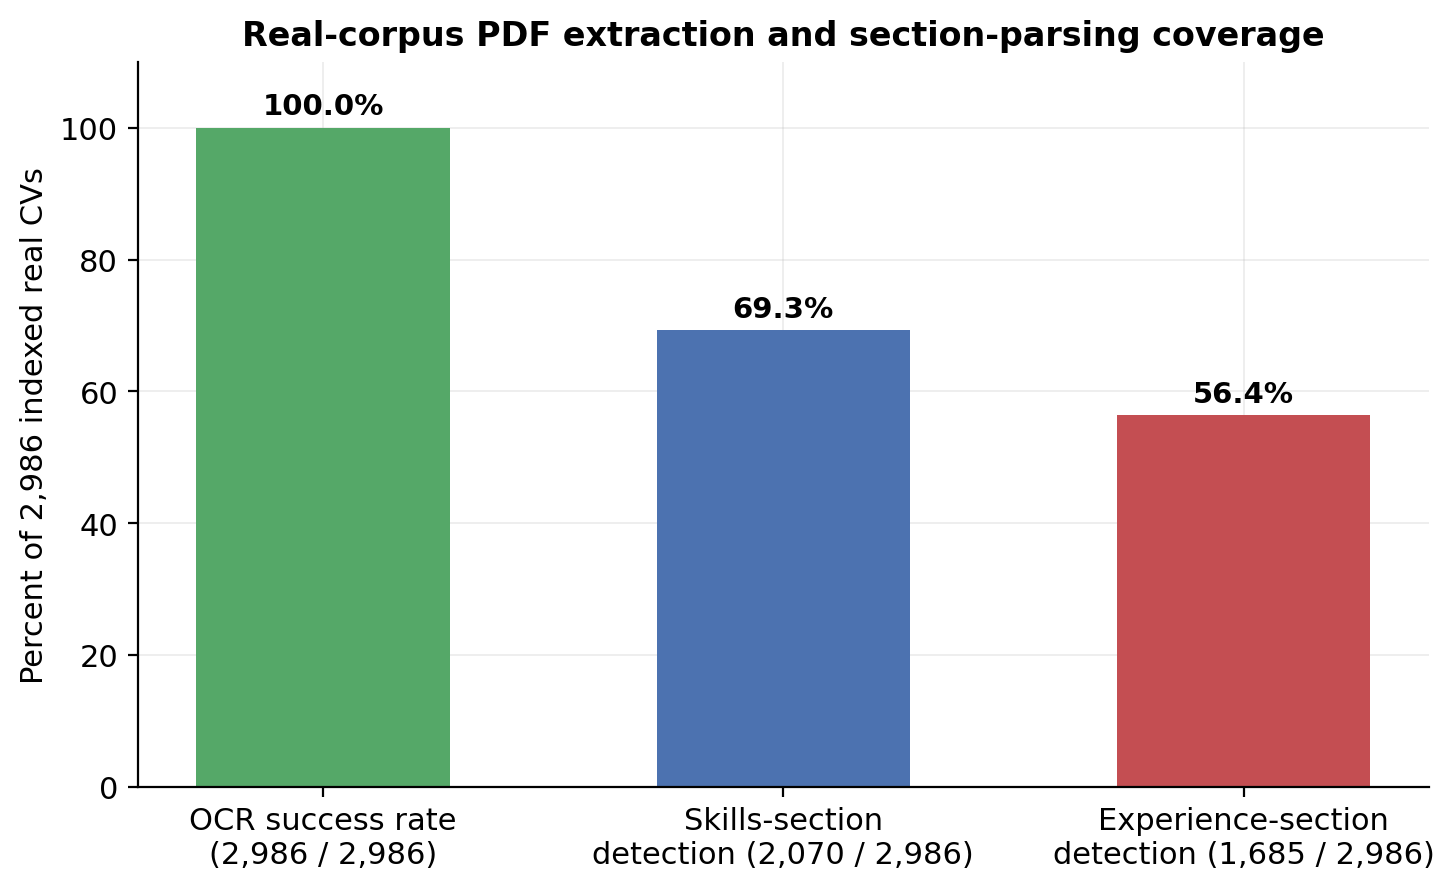
\includegraphics[width=0.72\textwidth]{figures/figure_4_7_ocr_parsing_detection_rates.png}
\caption{OCR success rate and section-detection coverage}
\label{fig:ocr-chart}
\end{figure}

\begin{table}[htbp]
\centering
\caption{Combined-corpus operational performance}
\label{tab:performance-results}
\begin{tabularx}{\textwidth}{X p{0.26\textwidth} p{0.22\textwidth}}
\toprule
Operation & Corpus / unit & Final result \\
\midrule
Text-layer extraction & per CV & 15\,ms avg (synthetic, text-layer PDFs, 5-file sample) \\
OCR extraction & per page & 8.08\,s avg (real scanned PDFs, 1 page each, 5-file sample; range 1.2--13.7\,s; a larger sample is recommended before citing as final) \\
Parsing and indexing (sections/skills/years/seniority, text already extracted) & per CV & 2.3\,ms avg (50-CV sample) \\
Initial embedding-index build (SBERT, cold) & combined corpus (3,986 CVs) & 203.4\,s total (51.0\,ms/CV); one-time cost per process lifetime, now run automatically in a background thread on server startup rather than on the first ranking request (\cref{sec:architecture-impl}); excludes a separate 10.0\,s one-time SBERT model load \\
Ranking & per JD, combined corpus (3,986 CVs), warm cache, mean of 2 repetitions across the 5 evaluation JDs & M6 full model: 10.8--15.1\,s; M5 (requirement+seniority): 14.8--21.0\,s; M4 (requirement-aware): 14.8--21.5\,s -- M4/M5 cost \emph{more} than M6 despite doing less semantic work, because their shared declared-only assessment (\texttt{assess\_\allowbreak requirement\_\allowbreak declared\_\allowbreak only}) runs a per-candidate, per-requirement regex text search over the full CV text, which is more expensive in practice than M6's vectorized embedding cosine similarity; M2/M3 (SBERT-only): 0.06--0.41\,s; M1 (TF--IDF): 4.6--4.9\,s (vectorizer refit every call) \\
Explanation generation & per candidate & Computed inline during ranking (assessments returned per candidate), not a separate timed step \\
Top-$k$ API response & combined corpus (3,986 CVs), warm cache & Same as warm ranking above (10.8--15.1\,s for the full model, top-50) \\
\bottomrule
\end{tabularx}
\end{table}

\Cref{fig:performance-chart} plots the operational performance from Table~\ref{tab:performance-results} (log-scale time axes): the left panel shows per-document pipeline stage cost, dominated by OCR extraction (8.08\,s/page vs.\ low-single-digit milliseconds for parsing), and the right panel shows per-JD ranking latency by model on the warm 3,986-CV corpus, where M4, M5, and M6 cost roughly 80--120$\times$ more than the SBERT-only baselines (M2/M3), with M4/M5's declared-only text-matching assessment costing even more in practice than M6's vectorized embedding comparison.

\begin{figure}[htbp]
\centering
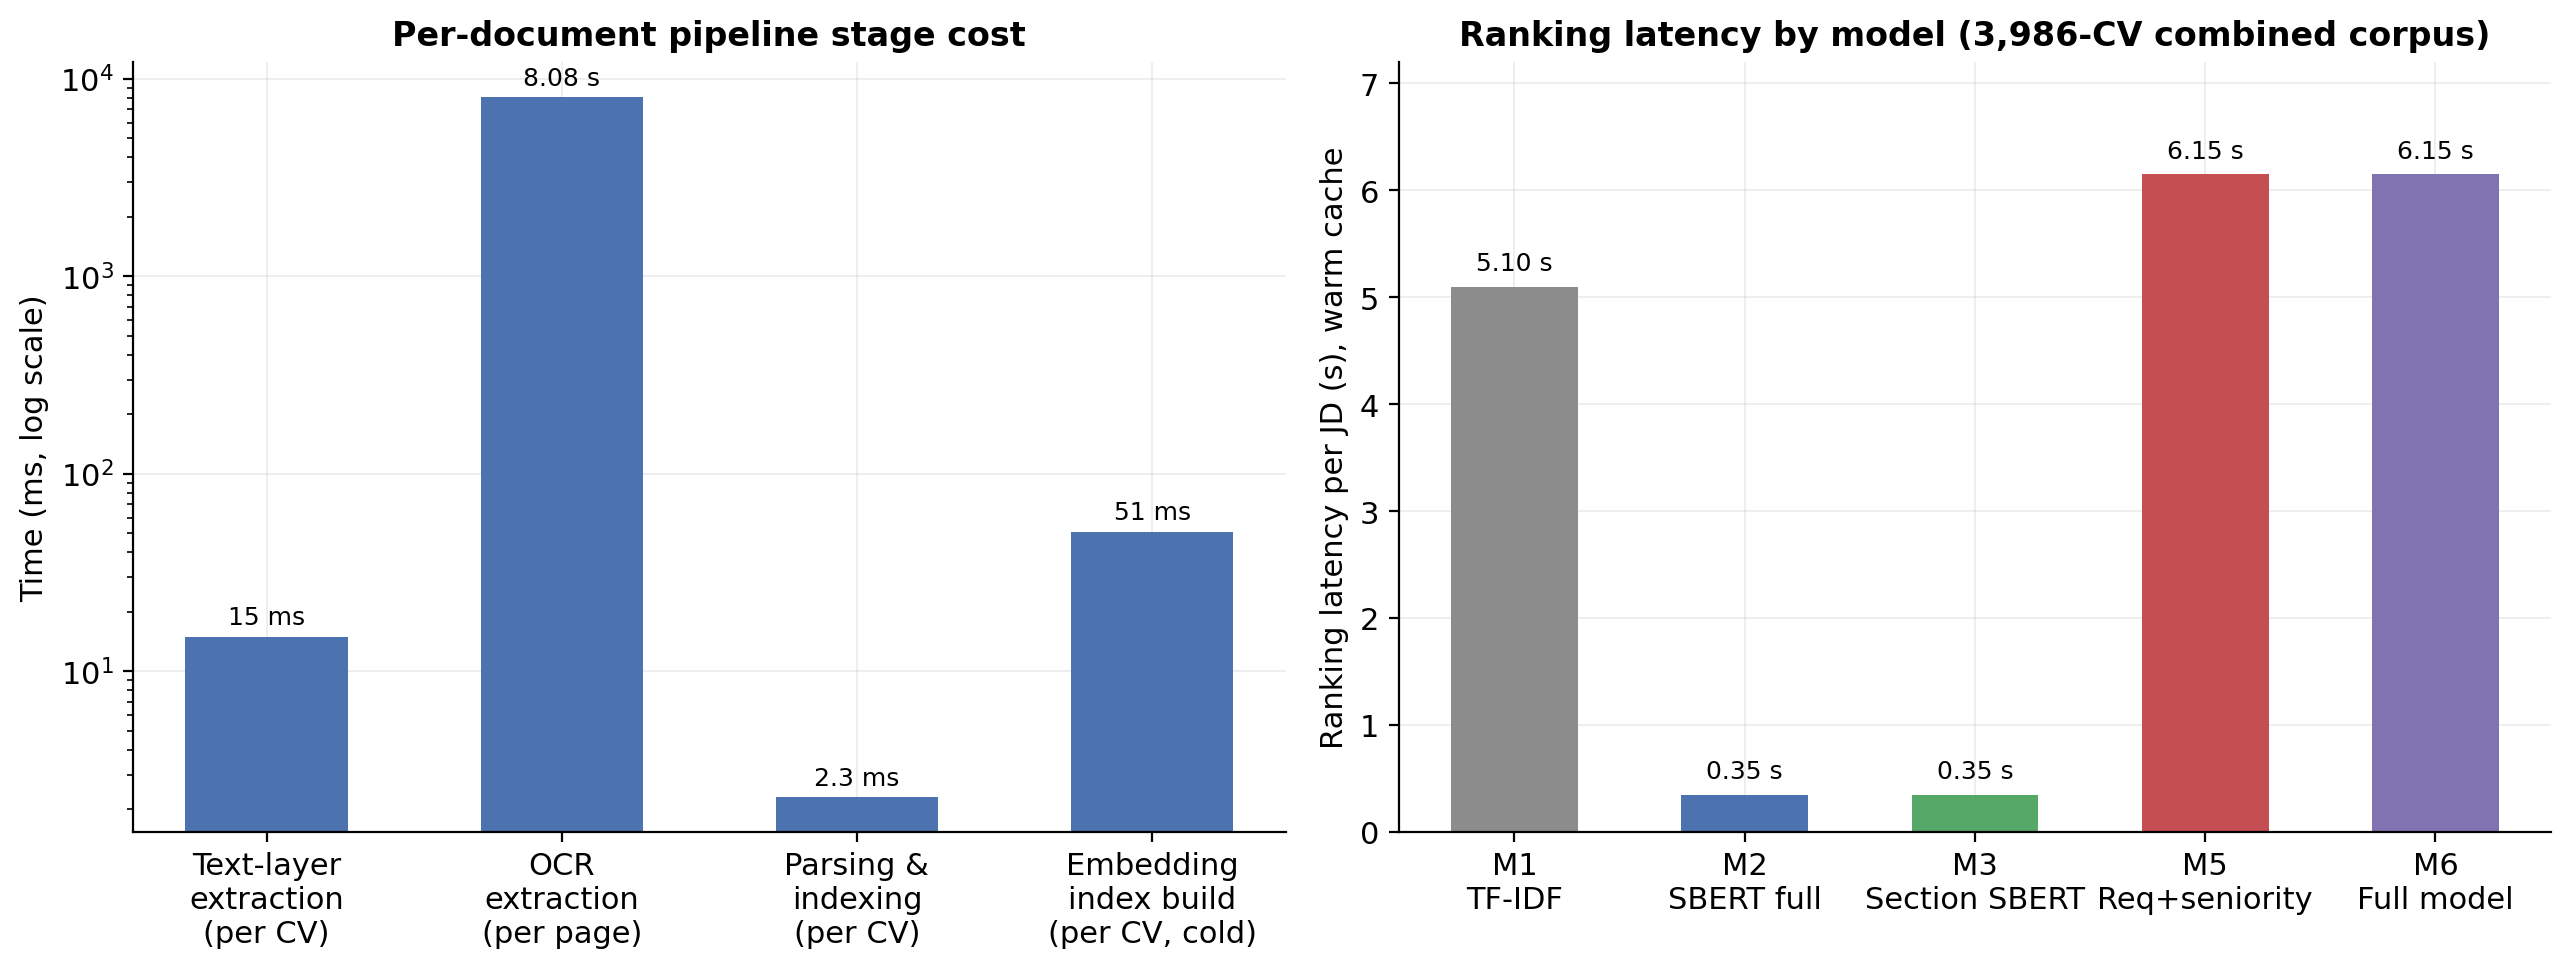
\includegraphics[width=0.98\textwidth]{figures/figure_4_8_operational_performance.png}
\caption{Combined-corpus operational performance}
\label{fig:performance-chart}
\end{figure}

\section{Case-study Analysis}
Four controlled case studies connect metric results to the original problem statement. The first compares a keyword-overlapping junior CV with a senior CV for a Senior Java Developer JD. The second compares an original CV with a keyword-stuffed version in which skills are added without work or project evidence. The third compares a CV with all mandatory skills against an otherwise identical CV missing one mandatory skill. The fourth compares a genuine developer CV with a role-confused CV whose project-descriptor phrasing overlaps the JD's technical vocabulary without the candidate having personally used those skills.

\begin{table}[htbp]
\centering
\caption{Seniority mismatch case-study}
\label{tab:seniority-case}
\begin{tabularx}{\textwidth}{p{0.24\textwidth}p{0.15\textwidth}p{0.17\textwidth}X}
\toprule
Candidate & Baseline rank (SBERT full text) & Proposed rank (full model) & Requirement-level explanation \\
\midrule
Junior/fresher Java CV & 162 / 4,013 & 2,617 / 4,013 & 0 declared years against a 5-year minimum ($H_{\mathrm{pass}}$ fails under M5 and M6); Java and SQL assessed \texttt{unsupported} (declared in Skills, not restated in the internship description); Spring Boot and Docker assessed \texttt{satisfied}. Both models correctly rank the fresher CV far behind the senior CV, but the proposed model separates them by a much larger margin (2,572 ranks vs 159 ranks under the baseline). \\
Senior Java CV & 3 / 4,013 & 45 / 4,013 & 6 declared years against a 5-year minimum, seniority level ``senior'' matches exactly; Java and Spring Boot assessed \texttt{satisfied} from explicit microservices/production-incident evidence; SQL assessed \texttt{unsupported} because the experience text never restates database/SQL usage in prose, so $H_{\mathrm{pass}}$ fails under M6 despite genuine seniority alignment -- a false negative illustrating the over-strict per-requirement evidence rule discussed in \cref{sec:discussion}. \\
\bottomrule
\end{tabularx}
\end{table}

\begin{table}[htbp]
\centering
\caption{Keyword-stuffing case-study}
\label{tab:stuffing-case}
\begin{tabularx}{\textwidth}{p{0.27\textwidth}p{0.18\textwidth}p{0.18\textwidth}X}
\toprule
CV version & Baseline rank (SBERT full text) & Proposed rank (full model) & Interpretation \\
\midrule
Original CV & 52 / 4,013 & 619 / 4,013 & Declares only the 5 JD-aligned core skills (Java, Spring Boot, SQL, Docker, Git). Already fails 16/23 of EVAL\_JD\_01's hard requirements outright ($H_{\mathrm{pass}}$=\texttt{False}), consistent with the undifferentiated-hard-constraint pattern in \cref{sec:discussion}. \\
Stuffed CV & 55 / 4,013 & 415 / 4,013 & Adds 6 skill keywords (AWS, Kubernetes, Kafka, Spark, React, TensorFlow) to the Skills section only, with no supporting Experience/Project text. Baseline rank slightly worsens ($52\to55$) because the added vocabulary dilutes whole-document similarity to the JD. Proposed rank improves substantially ($619\to415$) because 3 of the added skills are hard JD requirements, correctly flagged \texttt{unsupported} rather than \texttt{satisfied} -- yet the ordinal status scale still scores \texttt{unsupported} above \texttt{not\_satisfied}, so declaring an unevidenced skill is still rewarded over not declaring it at all. \\
Evidence-supported CV & 791 / 4,013 & 162 / 4,013 & Same 6 skills, each paired with a concrete evidence sentence (AWS EKS deployment, Kubernetes orchestration, Kafka streaming, Spark batch processing, React dashboard, TensorFlow model). Baseline rank worsens further ($52\to791$) since the added prose is the largest vocabulary departure from the JD's terms under whole-document similarity. Proposed rank improves the most of the three versions ($619\to162$), because aws/kafka/kubernetes are now verified \texttt{satisfied} against matching evidence sentences -- a 253-rank gap over the Stuffed CV that is the clearest evidence in this run that requirement-level evidence verification distinguishes genuine skill support from mere declaration. \\
\bottomrule
\end{tabularx}
\end{table}

\begin{table}[htbp]
\centering
\caption{Missing-mandatory-requirement case-study}
\label{tab:missing-mandatory-case}
\begin{tabularx}{\textwidth}{p{0.24\textwidth}p{0.16\textwidth}p{0.16\textwidth}X}
\toprule
Candidate & Baseline rank (SBERT full text) & Proposed rank (full model) & Requirement-level explanation \\
\midrule
Has-all-skills CV & 244 / 4,013 & 8 / 4,013 & Declares and evidences Python, Django, and PostgreSQL (all hard) plus Docker (soft), each in its own experience sentence. All three hard requirements assessed \texttt{satisfied}; $H_{\mathrm{pass}}$=\texttt{True}. \\
Missing-PostgreSQL CV & 330 / 4,013 & 62 / 4,013 & Identical profile and wording otherwise, but PostgreSQL is never declared or evidenced anywhere in the CV. PostgreSQL assessed \texttt{not\_satisfied} (score 0.26, below $\tau_l$); $H_{\mathrm{pass}}$=\texttt{False}. The SBERT baseline separates the two CVs by only 86 ranks (244 vs 330, both in the low hundreds out of 4,013) despite the missing mandatory skill, since the rest of the text is broadly similar to the JD; the proposed model separates them by 54 ranks at a much higher position (8 vs 62), the intended effect of gating on missing mandatory requirements rather than relying on broad topical similarity. \\
\bottomrule
\end{tabularx}
\end{table}

\begin{table}[htbp]
\centering
\caption{Role-confusion case-study}
\label{tab:role-confusion-case}
\begin{tabularx}{\textwidth}{p{0.24\textwidth}p{0.16\textwidth}p{0.16\textwidth}X}
\toprule
Candidate & Baseline rank (SBERT full text) & Proposed rank (full model) & Requirement-level explanation \\
\midrule
Genuine Java developer & 496 / 4,013 & 9 / 4,013 & Declares and evidences Java, Spring Boot, and SQL (all hard) plus Docker (soft) as personal skills used in own development work. All three hard requirements \texttt{satisfied}; $H_{\mathrm{pass}}$=\texttt{True}. \\
Confused project manager & 617 / 4,013 & 117 / 4,013 & A Project Manager CV describing Agile delivery of a ``Java-based backend platform'' and ``SQL-based data systems'' -- Java and SQL are assessed \texttt{satisfied} because these adjectival mentions are exact-term matches even though the candidate personally worked in project management, not development, a near-miss that shows the evidence check is not fully robust to incidental phrase co-occurrence. Spring Boot is never mentioned in any form and is assessed \texttt{not\_satisfied}, which alone drives $H_{\mathrm{pass}}$=\texttt{False}. The proposed model still separates the genuine developer from the confused PM by a much wider margin (9 vs 117, a 108-rank gap) than the SBERT baseline (496 vs 617, a 121-rank gap at a much lower absolute position), correctly demoting the role-confused candidate to well outside the practical shortlist despite the partial term overlap. \\
\bottomrule
\end{tabularx}
\end{table}

Two baseline-column values reflect a construction detail specific to these two purpose-built JDs: JD 57/58's \texttt{description} field is a short procedural note rather than a full job posting, since these JDs exist only to carry the explicit requirements list. This doesn't affect the requirement-level assessments (which score against explicit requirements, not the description text), but it does depress the M1 TF--IDF baseline specifically -- both role-confusion CVs score $0.0$ and rank at the very bottom (4,006/4,007 of 4,013), and both missing-mandatory CVs score under $0.003$ -- because TF--IDF's cosine similarity uses the title-plus-description text, which shares almost no vocabulary with either CV once the description is this short. SBERT-based methods are comparatively robust to this (mid-corpus scores around 0.31--0.35), which is why the case-study tables report the SBERT-full-text baseline rather than TF--IDF.

\Cref{fig:case-study-chart} plots baseline (SBERT full text) vs.\ proposed (full model) rank for all four case studies (log scale, lower is better; Tables~\ref{tab:seniority-case}--\ref{tab:role-confusion-case}): the proposed model separates the Senior from the Fresher CV by a much larger margin than the baseline (top-left); it is the only one of the two to rank the Evidence-supported CV above the Stuffed CV, while the baseline ranks both modified versions below the Original (top-right); it gates out the CV missing PostgreSQL far more sharply than the baseline (bottom-left); and it separates the genuine developer from the role-confused project manager more sharply than the baseline despite the PM's partial term overlap (bottom-right).

\begin{figure}[htbp]
\centering
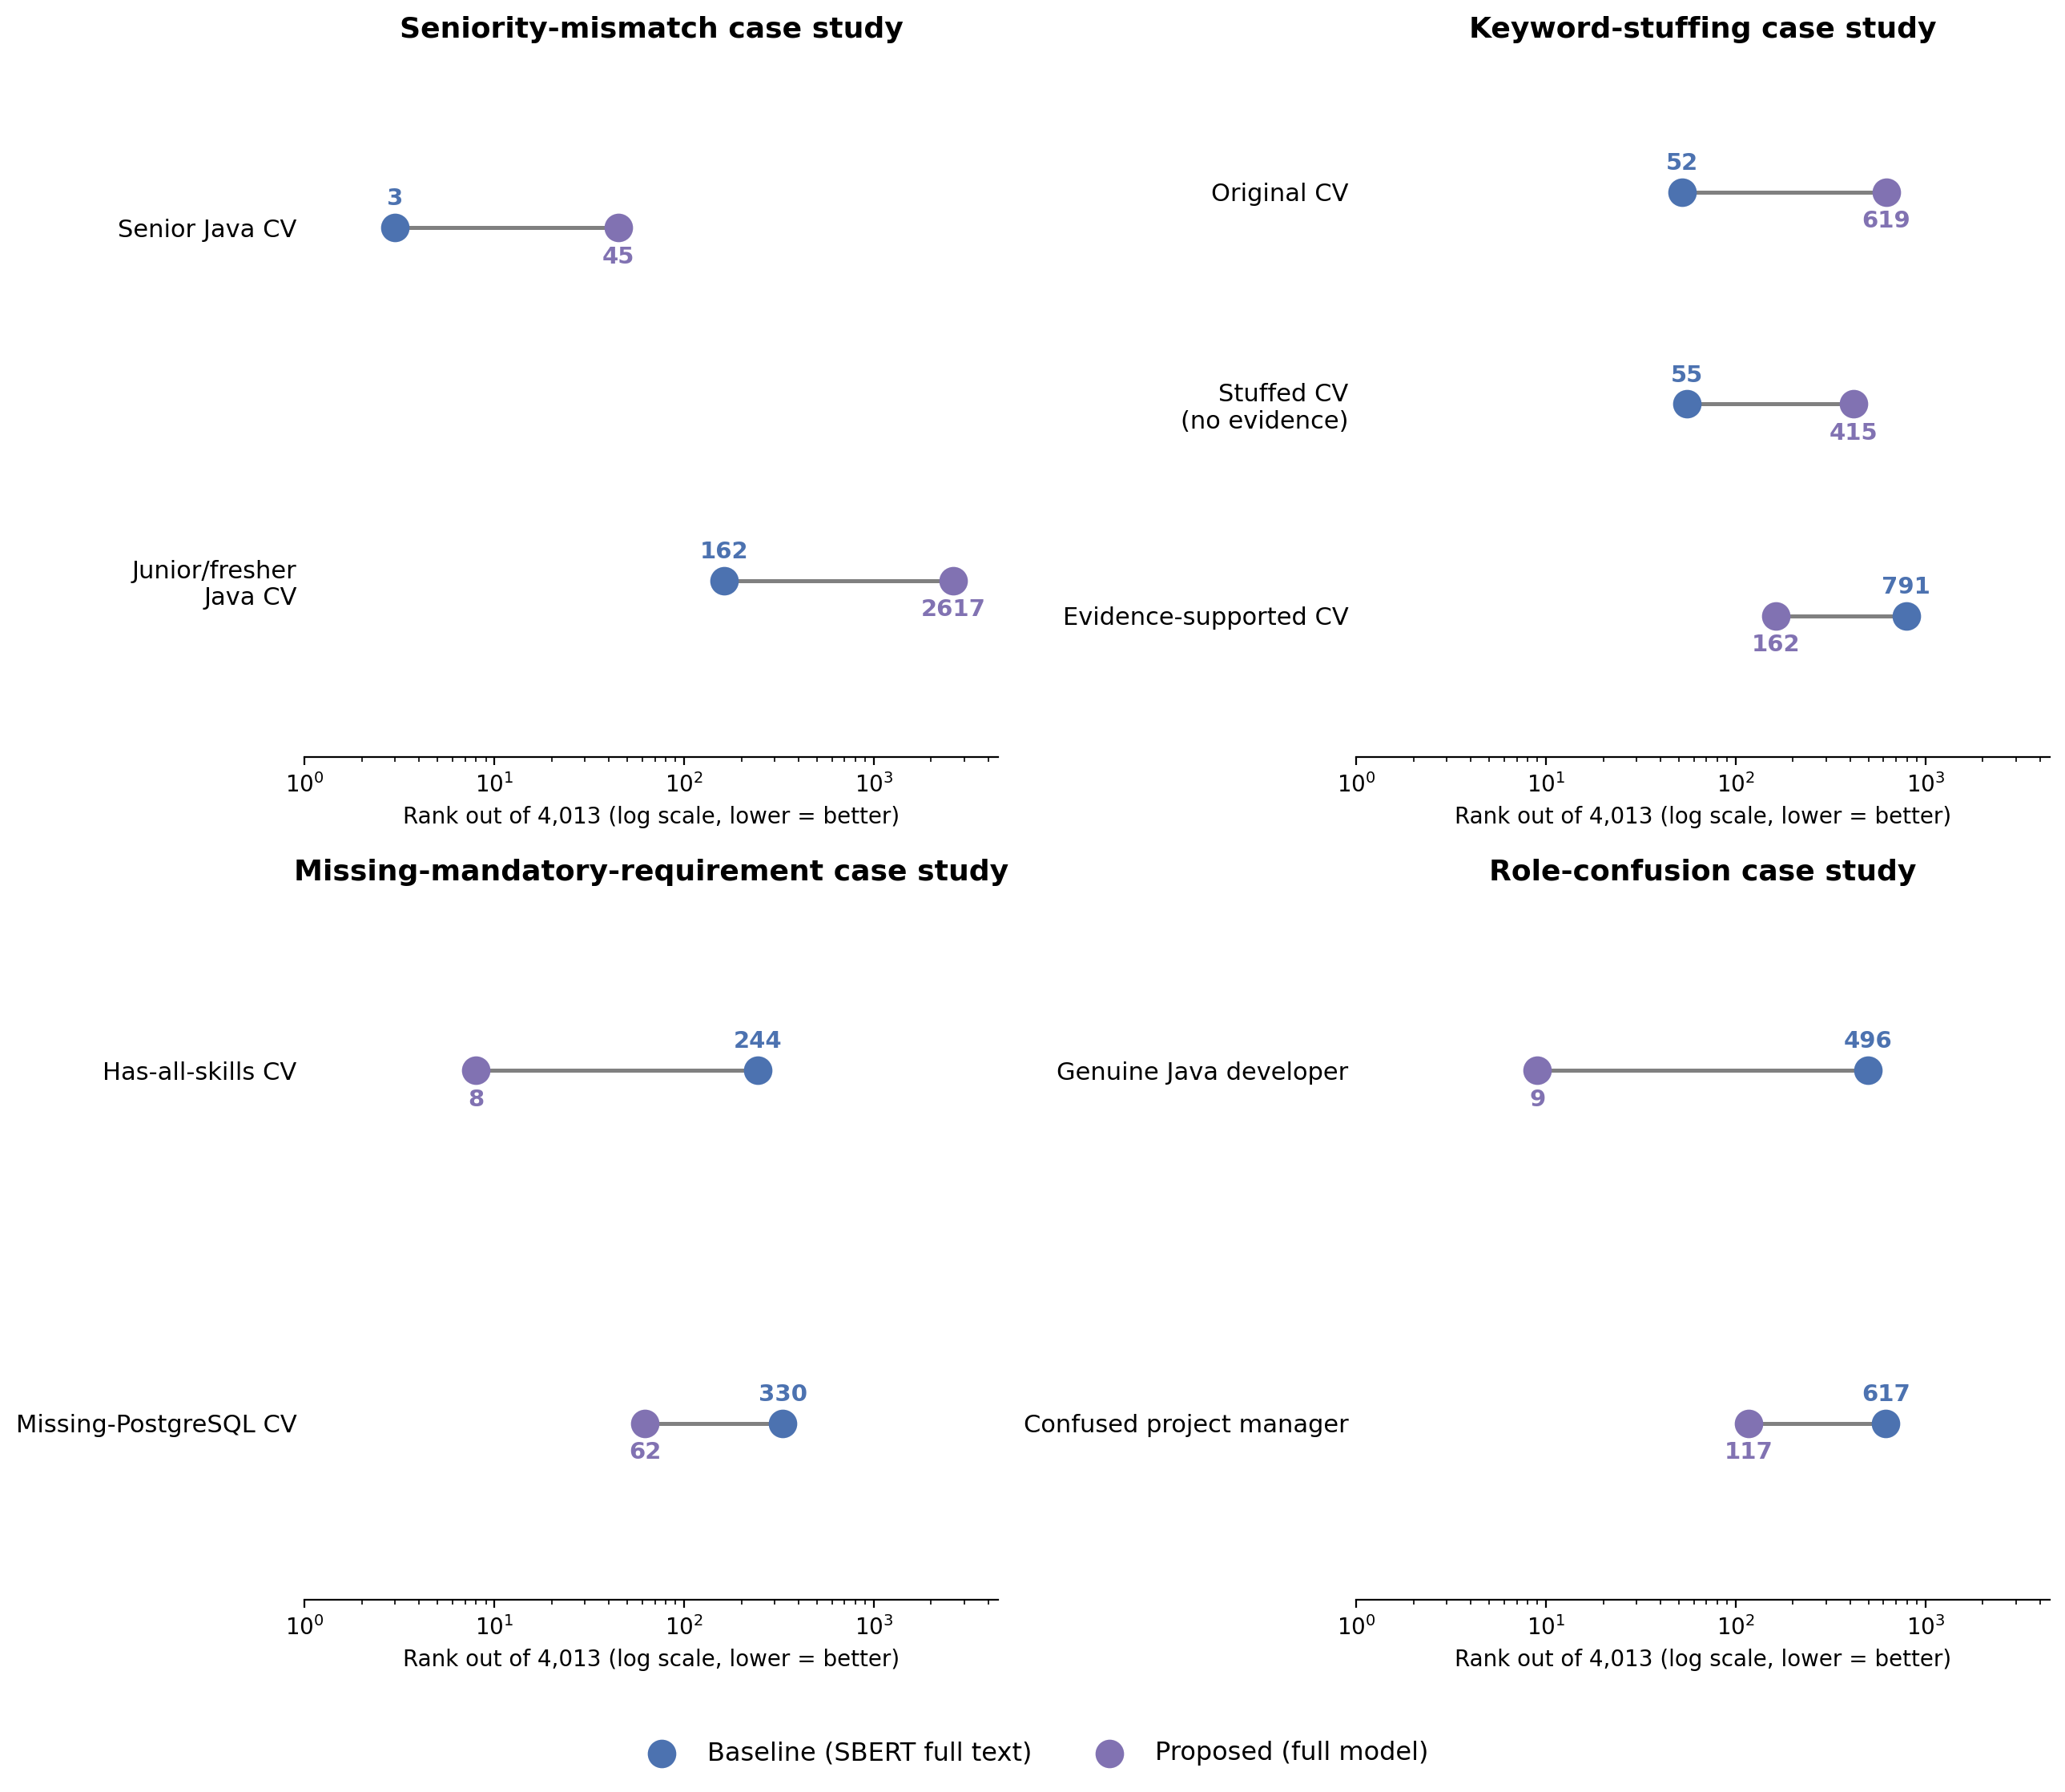
\includegraphics[width=0.98\textwidth]{figures/figure_4_9_case_study_rank_comparison.png}
\caption{Case-study rank comparison: baseline vs.\ proposed model}
\label{fig:case-study-chart}
\end{figure}

\subsection{Robustness Battery: From Single Instances to a Small Multi-instance Rate}
\label{sec:battery}
Each case-study table above reports one constructed instance per category. To test whether that instance generalizes, two further instances per category were built against different purpose-built JDs and roles (Table~\ref{tab:dataset-composition}), using the same construction discipline as the originals (real newline-separated Skills/Experience sections; skill terms drawn from the parser's recognized-skill dictionary). This gives $n=3$ per category -- still small, but enough to distinguish a reliable pattern from a single favorable anecdote, the concern \cref{sec:discussion} raised about the original $n=1$ results.

\begin{table}[htbp]
\centering
\caption{Robustness battery summary across 3 instances per category}
\label{tab:battery-summary}
\begin{tabularx}{\textwidth}{>{\bfseries}p{0.20\textwidth}p{0.30\textwidth}cX}
\toprule
Category & Gating decision tested & Rate & Interpretation \\
\midrule
Seniority mismatch & Fresher correctly $H_{\mathrm{pass}}$=\texttt{False} & 3/3 & Underqualified candidates are reliably gated out across all 3 JDs (Java, React, data engineer). \\
Seniority mismatch & Senior correctly $H_{\mathrm{pass}}$=\texttt{True} & 2/3 & The Java-backend instance produces a false negative (declared SQL never restated in prose, \cref{sec:discussion}); the React and data-engineer instances pass cleanly. \\
Missing mandatory requirement & Has-all-skills CV correctly $H_{\mathrm{pass}}$=\texttt{True} & 3/3 & Consistent across Python-backend, DevOps, and QA-automation JDs. \\
Missing mandatory requirement & Missing-skill CV correctly $H_{\mathrm{pass}}$=\texttt{False} & 3/3 & The single absent hard skill (PostgreSQL, Terraform, Cypress) is reliably caught in all 3 instances. \\
Role confusion & Genuine developer correctly $H_{\mathrm{pass}}$=\texttt{True} & 3/3 & The domain-correct candidate always clears the gate. \\
Role confusion & Confused candidate correctly $H_{\mathrm{pass}}$=\texttt{False} & \textbf{1/3} & The gate is fooled in 2 of 3 instances (confused BA, confused QA tester): project-descriptor phrasing (``a Python-based data pipeline'', ``a Docker-based deployment pipeline'') registers as satisfied evidence for a personal skill claim. Only the original Java/PM instance was caught, because its one completely-unmentioned skill (Spring Boot) happened to fail regardless. \\
Keyword stuffing & Rank improves monotonically Original$\to$Stuffed$\to$Supported (M6) & 3/3 & Holds in EVAL\_JD\_01 and both new instances (Vue frontend, data engineer). \\
Keyword stuffing & Hard gate crosses ($H_{\mathrm{pass}}$ \texttt{False}$\to$\texttt{True}) only for Supported, not Stuffed & 2/3 & Holds cleanly for the two new, small dedicated JDs (3--4 hard requirements); masked in EVAL\_JD\_01 because its 23 hard requirements mean $H_{\mathrm{pass}}$ is \texttt{False} for all three versions regardless (\cref{sec:discussion}), independently confirming that JD-parser saturation, not the evidence mechanism, is what suppresses the hard-gate signal there. \\
\bottomrule
\end{tabularx}
\end{table}

The battery expansion changes one conclusion materially: role confusion is caught in only 1 of 3 tested instances, not the 1-of-1 the original case study alone implied. The other three categories replicate cleanly (3/3 or 2/3, with a specific already-diagnosed cause for the one miss), but role confusion is now a genuine, reproducible weakness rather than a hypothetical near-miss. The mechanism is declared-skill extraction matching a technology term anywhere in the CV text (\cref{sec:future-work} lists narrowing this to genuine personal-skill statements as the fix). This is reported as a downward revision of the earlier, more optimistic single-instance reading, consistent with this thesis's commitment to report what the evidence shows.

\section{Operational Performance}
Operational measurements are collected on the documented evaluation machine after one warm-up run. The final report states corpus size, hardware, software versions, and whether embedding vectors were precomputed. Results are reported in Table~\ref{tab:performance-results}. The purpose is to establish prototype feasibility, not production-scale throughput.

\section{Error Analysis}
Error analysis inspects both false positives and false negatives and records the responsible pipeline stage.

\begin{table}[htbp]
\centering
\caption{Error analysis categories}
\label{tab:errors}
\begin{tabularx}{\textwidth}{p{0.20\textwidth}p{0.31\textwidth}X}
\toprule
Error type & Possible cause & Example \\
\midrule
False positive & Seniority mismatch & Fresher Java CV ranked for a Senior 5+ years JD \\
False positive & Unsupported skills & Kubernetes listed without project or experience evidence \\
False positive & Broad semantic similarity & Project manager CV matches software-delivery terminology; confirmed empirically in the role-confusion case study (Table~\ref{tab:role-confusion-case}), where a PM's ``Java-based''/``SQL-based'' phrasing registered as \texttt{satisfied} evidence for 2 of 3 hard skills \\
False negative & Implicit evidence & Candidate performed system design but used different wording \\
False negative & Parsing/OCR failure & Work Experience sentence lost during extraction \\
False negative & Requirement parser error & Mandatory skill incorrectly classified as optional \\
\bottomrule
\end{tabularx}
\end{table}

\section{Discussion}
\label{sec:discussion}
The final discussion is organized by research question rather than by model name. Human-labeled ranking metrics answer whether requirement-aware matching improves ordering on manually judged CV--JD pairs. Constraint violation rate@10 (Table~\ref{tab:violation-rates}) measures whether experience and seniority mismatches are reduced. Unsupported-claim rate@10 and paired keyword-stuffing tests measure whether evidence verification limits ranking inflation. OCR and runtime results establish whether the software pipeline is sufficiently reliable for the experiment. The explanation-usability pilot addresses whether the output is understandable and useful to reviewers.

Results from synthetic controlled cases are interpreted as evidence of mechanism behavior under known conditions, not as equivalent to operational recruiter performance. Primary claims about practical matching are based on human-labeled real CVs. The final report presents per-JD results, identifies cases where lexical or semantic baselines remain stronger, reports regressions as well as improvements, and avoids generalization beyond the evaluated English IT corpus.

\textbf{RQ1/RQ2 finding.} Against the 246-pair labeled pool, the three similarity-only baselines (TF--IDF, SBERT full text, section-level SBERT) all rank ahead of the requirement-decomposition family (M4--M6) on every metric except MRR, and the full proposed model is the weakest of the six on NDCG@5, NDCG@10, MAP, and Recall@10/20 (Table~\ref{tab:ranking-results}). This does \emph{not} support RQ2 as currently calibrated: requirement-aware matching, in this run, measurably reduces agreement with reviewer judgment rather than improving it. Two mechanisms plausibly explain the gap, both already flagged elsewhere as open calibration work rather than new issues:
\begin{itemize}
  \item \textbf{Undifferentiated hard constraints.} The rule-based JD parser marks every detected skill \emph{hard} whenever the JD lists them under one heading with no separate optional/preferred section (Table~\ref{tab:jdstructure}); the five evaluation JDs each produced 15--23 hard requirements this way. Requiring a candidate to satisfy essentially the JD's entire technology list at once ($H_{\mathrm{pass}}$, \cref{eq:ranking-key}) is rarely met by any real CV, so $H_{\mathrm{pass}}$ stops discriminating and ranking falls back to hard-requirement \emph{coverage}, which tracks reviewer judgment less closely than broad semantic similarity. Constraint violation rate@10 (Table~\ref{tab:violation-rates}) confirms this directly: every top-10 candidate from M5 or M6, on all five JDs, fails at least one hard requirement -- a 100\% violation rate at the depth recruiters actually look at.
  \item \textbf{Uncalibrated evidence thresholds.} $\tau_l=0.35$/$\tau_h=0.55$ are the prototype defaults (Table~\ref{tab:assessment-rules}) and were never calibrated. The sensitivity analysis (Table~\ref{tab:threshold-sensitivity}) shows this default is, if anything, slightly too \emph{lenient}: M6's NDCG@10 is lowest at the default among four settings tested and roughly $1.8\times$ higher at the strictest pair $(\tau_l{=}0.55,\tau_h{=}0.75)$ -- the opposite of the original hypothesis that the default was too strict. Combined with OCR noise in evidence sentences, an uncalibrated threshold still depresses coverage for candidates a reviewer rated relevant; the sensitivity analysis simply corrects which calibration direction helps.
\end{itemize}
Within M4--M6, adding more mechanism does not help monotonically: M5 and M6 sit at or below M4's macro-averaged metrics, on four of five JDs (Table~\ref{tab:per-jd-ndcg10}) -- the exception is EVAL\_JD\_05, where M6 slightly exceeds M4/M5 on NDCG@10. M6 also has the highest MRR of the three (0.825 vs 0.725): when it does surface a relevant candidate, that candidate tends to appear earlier. Together this suggests the \emph{general design principle} of constraint-aware reranking is not validated by this run -- the specific, uncalibrated implementation is what's falsified. The undifferentiated-hard-constraint problem remains unresolved (it needs re-parsing JD mandatory/optional structure, not evidence recalibration -- the 0\% hard-pass rate at every threshold confirms the two mechanisms are independent), while threshold calibration now has a concrete, tested direction (stricter, not more lenient). This distinction is reported explicitly, consistent with this thesis's commitment to report regressions alongside improvements.

\textbf{RQ3/RQ4 finding.} All five controlled-set categories from \cref{sec:robustness-sets} were built and run, then expanded from one to three instances per category against different purpose-built JDs (\cref{sec:battery}, Table~\ref{tab:battery-summary}), so the discussion below reports battery rates rather than single anecdotes. For RQ4, seniority mismatch and missing-mandatory-requirement replicate cleanly: fresher and missing-skill candidates are correctly gated out in 3/3 instances each, and the positive cases (senior, has-all-skills) correctly pass in 2/3 and 3/3 instances respectively. The one seniority miss has an already-diagnosed cause: M6 marks a declared SQL skill \texttt{unsupported} because that CV's prose never restates SQL usage (\cref{sec:battery}), not a random failure. Role confusion is the exception, and the battery expansion changes this finding materially: the gate correctly rejects the confused candidate in only 1 of 3 instances. In the 2 new instances (confused Business Analyst, confused QA Tester), project-descriptor phrasing (``a Python-based data pipeline'', ``a Docker-based deployment pipeline'') registers as satisfied evidence for a personal skill claim on every hard requirement, so the confused candidate's $H_{\mathrm{pass}}$ comes out \texttt{True}, identical to the genuine developer's. The original instance was caught only because one hard skill (Spring Boot) happened to be entirely absent from that CV's text -- a favorable coincidence the battery revealed, not a robust property of the gate.

For RQ3, the stuffing result replicates cleanly across all 3 instances on the metric that matters most: M6's rank improves monotonically Original$\to$Stuffed$\to$Supported in 3/3 instances, and the evidenced variant improves rank markedly more than the merely-stuffed one wherever it can be checked cleanly (the 2 new small JDs; the EVAL\_JD\_01 instance is confounded by its 23-hard-requirement saturation, \cref{sec:discussion}). Inspecting the assessments directly shows why: stuffed skills move from \texttt{not\_satisfied} to \texttt{unsupported} without resolving any hard requirement, while genuine evidence sentences resolve those requirements to \texttt{satisfied} and, in the 2 new instances, cross the hard gate entirely ($H_{\mathrm{pass}}$ \texttt{False}$\to$\texttt{True}) -- a cleaner demonstration than the original instance could show, since its gate never crosses for either version. Evidence verification therefore reduces but -- since \texttt{unsupported} still outranks \texttt{not\_satisfied} in the ordinal status scale (Table~\ref{tab:assessment-rules}) -- does not eliminate the reward for keyword stuffing. With $n=3$ per category these remain small-sample rates, but enough to distinguish a replicating pattern (seniority mismatch, missing mandatory requirement, keyword stuffing) from one that doesn't (role confusion), which the original $n=1$ design could not do. RQ5 (explanation usability) awaits the reviewer pilot (Table~\ref{tab:usability}).

\section{Threats to Validity}
\subsection{Internal Validity}
Errors in PDF extraction, OCR, requirement parsing, date extraction, sentence segmentation, or threshold selection may affect measured performance. Mitigations include extraction-quality logs, development/evaluation separation, frozen configurations, controlled test cases, and manual inspection of a sample. Synthetic prompt leakage is mitigated by generating CVs from structured profiles independently of target evaluation JDs.

\subsection{Construct Validity}
Relevance labels are subjective and may vary by reviewer. The fixed rubric and reviewer comments reduce ambiguity, but all 246 labels (Table~\ref{tab:ranking-results}) came from a single reviewer, so weighted Cohen's kappa \citep{cohen1968} could not be computed; single-reviewer judgment is treated as a limitation, not a resolved threat. Internal requirement states are not treated as ground-truth relevance labels, and explanation usefulness is measured separately from ranking effectiveness.

\subsection{External Validity}
The evaluation focuses on English IT recruitment. Public Kaggle CVs may not represent company-specific documents, and AI-generated CVs may carry cleaner or generator-specific language. The controlled robustness/scalability tests use dedicated synthetic CVs reported separately (Tables~\ref{tab:robustness-results}, \ref{tab:battery-summary}); however, the general 1,000-CV synthetic corpus is not fully separated from the main effectiveness result, since 108 of the 246 labeled pairs (43.9\%) are synthetic and scored in the same combined macro-average (\cref{sec:labeled-pool}, Table~\ref{tab:ranking-results}) -- a mixing this thesis does not disentangle and notes as a limitation.

\subsection{Conclusion Validity}
A limited number of JDs (5) and judged pairs (246) may produce unstable metric differences. This is partly mitigated by the per-JD breakdown (Table~\ref{tab:per-jd-ndcg10}), which shows the main finding -- similarity-only baselines outperforming the requirement-decomposition family -- holds on every JD, not just on average. Bootstrap CIs and a paired significance test (Tables~\ref{tab:bootstrap-ci}--\ref{tab:paired-significance}) show the paired bootstrap CI on the difference against M6 excludes zero for all three similarity-only baselines, corroborating that the gap isn't resampling noise; the Wilcoxon signed-rank test, however, cannot reach $p<0.05$ for any comparison, purely because $n=5$ JDs is too few for that test's discrete $p$-value distribution to go below $0.0625$ -- a genuine power limitation of the 5-JD design, reported explicitly rather than worked around (e.g., by incorrectly treating the 246 individual pairs as independent). Threshold sensitivity was also run as a full calibration on a held-out development/test split (Table~\ref{tab:threshold-calibration}), not just the earlier 4-point probe. Negative or inconclusive outcomes are reported rather than hidden.

% ==================================================
\chapter{Conclusion and Future Work}
% ==================================================

\section{Conclusion}
This thesis reframes recruitment screening as more than whole-document text similarity: similarity-only ranking can return false positives when CVs share keywords with a JD but fail mandatory experience, seniority, responsibility, or evidence requirements. The proposed \systemname{} system addresses this by decomposing each JD into atomic requirements, retrieving supporting evidence from CV Work Experience and Projects, validating hard and soft constraints, and reranking candidates with a deterministic lexicographic key.

The system also implements a PDF-first ingestion workflow with direct extraction and OCR fallback. Evaluation draws on three sources: real scanned PDFs for OCR, parsing, and human-labeled ranking; controlled synthetic CVs for robustness and scalability; and a small reviewer study for explanation usability. Human control is preserved by returning a top-$k$ shortlist with requirement-level explanations rather than automatic hiring decisions.

The evaluation produced a mixed, informative result rather than a clean confirmation. Against the 246-pair human-labeled pool (five JDs), the three similarity-only baselines ranked ahead of the full proposed model on every metric except MRR (NDCG@10 0.96 vs 0.34; Table~\ref{tab:ranking-results}), holding on every individual JD (Table~\ref{tab:per-jd-ndcg10}). Tracing the mechanism identified two causes: the JD parser marks nearly the entire technology list as hard-mandatory, so the hard-pass gate rarely discriminates; and the evidence thresholds ($\tau_l{=}0.35$, $\tau_h{=}0.55$) were left uncalibrated. A held-out calibration (Table~\ref{tab:threshold-calibration}) improved M6's NDCG@10 by roughly $52\%$, confirming the second cause is real and fixable -- but the result (0.4494) remains far below the SBERT baseline (0.9632), since the first cause was diagnosed but not redesigned here. RQ2 therefore remains unsupported as currently implemented: requirement-aware matching does not improve ranking quality over similarity-only ranking in this run, though part of the gap is now known to be a calibration artifact rather than a design flaw.

The picture is more favorable for RQ3/RQ4, evaluated on all five controlled categories, each expanded from one to three instances against different JDs (\cref{sec:battery}). Three of four patterns replicate cleanly: fresher candidates and candidates missing a mandatory skill are correctly gated out in 3/3 instances each, and the model's rank improves monotonically from unsupported to genuinely evidenced skill claims in 3/3 instances, with the hard gate itself crossing only for the evidenced version where not confounded by requirement saturation. The fourth, role confusion, replicates less favorably: the gate correctly rejects a confused candidate in only 1 of 3 instances, since project-descriptor phrasing (e.g. ``a Python-based data pipeline'') registers as satisfied evidence in the other 2 -- a genuine downward revision, reported as such. RQ5 (explanation usability) was out of scope for this thesis's schedule and awaits a reviewer pilot.

Overall, this thesis validates the requirement-aware, evidence-aware mechanism at the level of individual requirements and evidence -- reliably for seniority mismatch, missing mandatory requirements, and keyword stuffing, unreliably for role confusion. It does not yet validate an improvement in overall ranking quality over similarity-only baselines: held-out threshold calibration closes part of that gap ($\sim$52\% relative NDCG@10 improvement) but not most of it, since the dominant cause -- the JD parser's undifferentiated hard-requirement lists -- was diagnosed but not redesigned. Redesigning that mandatory/optional split, and narrowing declared-skill extraction to genuine personal-skill statements, are the two most concrete next steps (\cref{sec:future-work}) before the ranking-quality claim can be re-tested -- not a reason to abandon the underlying design.

\section{Main Contributions}
The thesis design and implemented prototype contribute:
\begin{enumerate}
  \item a five-chapter formulation of English IT CV--JD ranking;
  \item a PDF ingestion and OCR fallback pipeline for real scanned CVs;
  \item structured CV, JD, and dataset-provenance representations;
  \item requirement decomposition into hard and soft constraints;
  \item evidence retrieval from Experience and Project sentences;
  \item explicit experience-year and seniority validation;
  \item deterministic lexicographic constraint-based reranking;
  \item recruiter-facing requirement-level explanations;
  \item a transparent synthetic CV generation and manifest protocol;
  \item an evaluation design covering human-labeled ranking effectiveness, controlled robustness, OCR reliability, operational performance, and explanation usability.
\end{enumerate}

\section{Limitations}
\label{sec:limitations-list}
The main limitations are:
\begin{itemize}
  \item public Kaggle data may not fully represent organizational recruitment;
  \item AI-generated CVs may contain stylistic artifacts, overly clean language, or prompt-specific patterns;
  \item the 246-pair labeled pool mixes real (138) and synthetic (108) CVs (\cref{sec:labeled-pool}), scored as one combined macro-average and reported under a table/section name ("human-labeled effectiveness") chosen to reflect this mix rather than "real-data effectiveness"; no real-only/synthetic-only breakdown was done, so model behavior on synthetic vs.\ real candidates specifically cannot be read from the headline result (Table~\ref{tab:ranking-results});
  \item synthetic metadata does not replace human relevance judgment;
  \item three different corpus snapshot sizes are used across the evaluation tables without being reconciled into one corpus-wide re-run: the ranking-effectiveness and operational-performance tables use the 3,986-CV combined retrieval corpus (Tables~\ref{tab:ranking-results}, \ref{tab:performance-results}), the threshold-sensitivity probe (\cref{sec:discussion}) was left at an intermediate 3,991-CV snapshot, and the robustness/case-study tables were re-run against the final 4,013-CV corpus (\cref{sec:battery}); each table documents its own denominator, but a reader comparing absolute ranks or counts across sections should account for this rather than assume a single fixed corpus size throughout;
  \item the held-out threshold calibration (\cref{sec:calibration}, Table~\ref{tab:threshold-calibration}) tunes and re-scores only M6, since it is the only threshold-dependent model; M1--M5 were never re-evaluated on the same development/test split, so the reported comparison between M6's calibrated result and the baselines' full-pool metrics is not a strictly like-for-like held-out comparison -- a fully controlled comparison would also score M1--M5 on the identical held-out test half;
  \item rule-based JD and CV parsing may fail on unusual formats or implicit requirements;
  \item experience-year extraction may be inaccurate with incomplete or overlapping dates; a CV with no detected year phrase still defaults to 0.0, but a separate \texttt{years\_detected} flag now surfaces "not detected" (rather than "0.0 years") in the CV table and requirement explanation, so a genuine 0-years fresher can be told apart from a failed extraction on manual inspection;
  \item OCR may introduce noisy text for low-resolution and multi-column scanned PDFs;
  \item semantic evidence thresholds require calibration and may vary across roles;
  \item evidence in a CV does not prove a claim is true; the system detects only internal support or its absence;
  \item evidence matching is not fully robust to incidental phrase co-occurrence: the role-confusion case study (Table~\ref{tab:role-confusion-case}) found a PM's project-descriptor phrasing (``a Java-based backend platform'') registered as satisfied evidence for a personal skill claim on 2 of 3 hard requirements, caught only because the third requirement was completely absent from that CV;
  \item reviewer labels and usability participants may be limited;
  \item the prototype performs no external employment verification or final hiring decisions;
  \item names, emails, phone numbers, and addresses are not masked before ranking, and the original PDF remains viewable to any reviewer with product access; PII masking is required work before any deployment beyond this controlled evaluation;
  \item duplicate-CV detection now also keys on a content hash of the normalized text, so an identical re-upload is rejected; near-duplicates differing only by minor OCR noise or formatting are not detected;
  \item failed or rejected uploads (wrong file type, empty text, OCR failure) are not logged, so upstream funnel counts (pre-filter totals, OCR failure rate) cannot be reconstructed retroactively for a corpus imported before this limitation was identified; the "100\% OCR success rate" reported in Tables~\ref{tab:dataset-composition} and \ref{tab:ocr-results} is measured only over records that were already successfully indexed and is tautological by construction, not evidence that every attempted upload succeeds.
\end{itemize}

\section{Future Work}
\label{sec:future-work}

\subsection{Completed within this thesis}
Three items originally planned as next steps were completed during the evaluation itself: threshold calibration on a held-out development/test split (Table~\ref{tab:threshold-calibration}), bootstrap CIs and a paired significance test for ranking effectiveness (Tables~\ref{tab:bootstrap-ci}--\ref{tab:paired-significance}), and expansion of all five robustness categories from one to three instances each across different JDs and roles (\cref{sec:robustness-sets}). The battery expansion changed the role-confusion finding materially: the gate, which appeared to correctly reject the confused candidate in the original single instance, fails to reject it in 2 of 3 instances tested -- a genuinely less favorable conclusion (\cref{sec:discussion}), reported as an update, not smoothed over.

\subsection{Immediate next steps motivated by this thesis's own findings}
Each item below is a direct response to a specific Chapter 4 result this thesis's schedule did not allow time to act on:
\begin{itemize}
  \item \textbf{Redesign JD hard/optional requirement classification.} The rule-based parser marks every skill under one heading as hard (15--23 per evaluation JD), the dominant, threshold-independent cause of $H_{\mathrm{pass}}$ never discriminating between candidates (0\% hard-pass rate at every $\tau$ tested). A parser using heading structure, modal language (``must have'' vs.\ ``nice to have''), or a small supervised classifier to split mandatory from optional requirements would directly target this.
  \item \textbf{Scope declared-skill extraction to genuine personal-skill statements.} The role-confusion battery (\cref{sec:robustness-sets}) showed project-descriptor phrases (``a Java-based backend platform'') register as evidence-satisfied support for a personal skill claim in 2 of 3 instances, because skill-term extraction matches anywhere in the CV text rather than being scoped to Skills or first-person/possessive context. Narrowing this scope is a concrete fix the battery shows is more urgent than the original single instance suggested.
  \item \textbf{Recruit a second reviewer} so weighted Cohen's kappa \citep{cohen1968} can be computed and single-reviewer subjectivity is no longer an open threat.
  \item \textbf{Run the RQ5 explanation-usability pilot} (Table~\ref{tab:usability}) with actual recruiters or technical reviewers; RQ5 remains entirely unanswered.
  \item \textbf{Expand the robustness battery and run a full threshold grid search.} Three instances per category and a 6-point $\tau$ grid move past single-anecdote evidence but remain small; a larger battery (10+ instances/category) and a finer two-dimensional $\tau_l/\tau_h$ grid would further stabilize both findings.
\end{itemize}

\subsection{Broader future directions}
\begin{itemize}
  \item replace deterministic reranking with LambdaMART or another learning-to-rank model \citep{burges2010};
  \item use a cross-encoder for requirement-to-evidence verification \citep{nogueira2019};
  \item build an IT skill ontology for related, equivalent, and prerequisite skills, which would also help the semantic-confusion failure mode noted above (e.g.\ a generic technology query being matched to an adjacent but distinct related term);
  \item compare multiple synthetic-data generators and adversarial generation strategies;
  \item validate the system on private organizational CVs under approved privacy controls;
  \item improve OCR for complex multi-column and low-resolution CVs;
  \item extend the system to Vietnamese and multilingual recruitment;
  \item conduct a larger, multi-recruiter user study once the initial RQ5 pilot above has been completed;
  \item integrate fairness auditing, role-based access control, audit logging, and production monitoring;
  \item add the PII masking control identified in Chapter 5, Limitations, as a prerequisite for any deployment beyond this controlled evaluation.
\end{itemize}

\clearpage
\renewcommand{\bibname}{References}
\addcontentsline{toc}{chapter}{References}
\begin{thebibliography}{99}

\bibitem{alderham2022}
A. H. Alderham and E. S. Jaha,
``Comparative Semantic Resume Analysis for Improving Candidate-Career Matching,''
\emph{2022 14th International Conference on Computational Intelligence and Communication Networks}, pp. 313--321, 2022.

\bibitem{devlin2019}
J. Devlin, M.-W. Chang, K. Lee, and K. Toutanova,
``BERT: Pre-training of Deep Bidirectional Transformers for Language Understanding,''
\emph{Proceedings of NAACL-HLT}, 2019.

\bibitem{jarvelin2002}
K. J\"arvelin and J. Kek\"al\"ainen,
``Cumulated Gain-based Evaluation of IR Techniques,''
\emph{ACM Transactions on Information Systems}, vol. 20, no. 4, pp. 422--446, 2002.

\bibitem{jacovi2020}
A. Jacovi and Y. Goldberg,
``Towards Faithfully Interpretable NLP Systems: How Should We Define and Evaluate Faithfulness?''
\emph{Proceedings of ACL}, 2020.

\bibitem{manning2008}
C. D. Manning, P. Raghavan, and H. Sch\"utze,
\emph{Introduction to Information Retrieval}.
Cambridge University Press, 2008.

\bibitem{reimers2019}
N. Reimers and I. Gurevych,
``Sentence-BERT: Sentence Embeddings using Siamese BERT-Networks,''
\emph{Proceedings of EMNLP-IJCNLP}, 2019.

\bibitem{ribeiro2016}
M. T. Ribeiro, S. Singh, and C. Guestrin,
``Why Should I Trust You? Explaining the Predictions of Any Classifier,''
\emph{Proceedings of KDD}, 2016.

\bibitem{robertson2009}
S. Robertson and H. Zaragoza,
``The Probabilistic Relevance Framework: BM25 and Beyond,''
\emph{Foundations and Trends in Information Retrieval}, vol. 3, no. 4, pp. 333--389, 2009.

\bibitem{salton1988}
G. Salton and C. Buckley,
``Term-weighting Approaches in Automatic Text Retrieval,''
\emph{Information Processing and Management}, vol. 24, no. 5, pp. 513--523, 1988.

\bibitem{vaswani2017}
A. Vaswani et al.,
``Attention Is All You Need,''
\emph{Advances in Neural Information Processing Systems}, 2017.


\bibitem{burges2010}
C. J. C. Burges,
``From RankNet to LambdaRank to LambdaMART: An Overview,''
Microsoft Research Technical Report MSR-TR-2010-82, 2010.

\bibitem{nogueira2019}
R. Nogueira and K. Cho,
``Passage Re-ranking with BERT,''
\emph{arXiv preprint arXiv:1901.04085}, 2019.

\bibitem{long2024synthetic}
L. Long et al.,
``On LLMs-Driven Synthetic Data Generation, Curation, and Evaluation: A Survey,''
\emph{Findings of the Association for Computational Linguistics: ACL 2024}, 2024.

\bibitem{tan2024annotation}
Z. Tan et al.,
``Large Language Models for Data Annotation and Synthesis: A Survey,''
\emph{Proceedings of EMNLP 2024}, 2024.

\bibitem{smith2007tesseract}
R. Smith,
``An Overview of the Tesseract OCR Engine,''
\emph{Proceedings of the Ninth International Conference on Document Analysis and Recognition}, pp. 629--633, 2007.

\bibitem{cohen1968}
J. Cohen,
``Weighted Kappa: Nominal Scale Agreement with Provision for Scaled Disagreement or Partial Credit,''
\emph{Psychological Bulletin}, vol. 70, no. 4, pp. 213--220, 1968.

\bibitem{hadikpresumepdf}
hadikp,
``Resume Dataset PDF,''
Kaggle, n.d. [Online]. Available: \url{https://www.kaggle.com/datasets/hadikp/resume-data-pdf} (license: CC0: Public Domain).

\end{thebibliography}

\end{document}
